%%%%%%%%%%%%%%%%%%%%%%%%%%%%%%%%%%%%%%%%%
% UAThesis
% LaTeX Template
% Version 1.0 (01/09/15)
%
% Based on the template
%
% License:
% CC BY-NC-SA 3.0 (http://creativecommons.org/licenses/by-nc-sa/3.0/)
%
%%%%%%%%%%%%%%%%%%%%%%%%%%%%%%%%%%%%%%%%%

%----------------------------------------------------------------------------------------
%	PACKAGES AND OTHER DOCUMENT CONFIGURATIONS
%----------------------------------------------------------------------------------------

\documentclass[
  12pt,           % The default document font size, options: 10pt, 11pt, 12pt
  %oneside,       % Two side (alternating margins) for binding by default, uncomment to switch to one side
  english,        % Language option for the babel package
  onehalfspacing,  % Single line spacing, alternatives: onehalfspacing or doublespacing
  %draft,         % Uncomment to enable draft mode (no pictures, no links, overfull hboxes indicated)
  %nolistspacing, % If the document is onehalfspacing or doublespacing, uncomment this to set spacing in lists to single
  %liststotoc,    % Uncomment to add the list of figures/tables/etc to the table of contents
  %toctotoc,      % Uncomment to add the main table of contents to the table of contents
  %parskip,       % Uncomment to add space between paragraphs
]{UAThesis} % The class file specifying the document structure

%----------------------------------------------------------------------------------------
%	THESIS INFORMATION
%----------------------------------------------------------------------------------------

\thesistitle{Deep Learning for 3D Perception:\\ Computer Vision and Tactile Sensing}
% Your thesis title, this is used in the title and abstract, print it elsewhere with \ttitle
\supervisor{Jose \textsc{Garcia-Rodriguez}}
% Your supervisor's name, this is used in the title page, print it elsewhere with \supname
\examiner{}
% Your examiner's name, this is not currently used anywhere in the template, print it elsewhere with \examname
\degree{Doctor of Philosophy}
% Your degree name, this is used in the title page and abstract, print it elsewhere with \degreename
\author{Alberto \textsc{Garcia-Garcia}}
% Your name, this is used in the title page and abstract, print it elsewhere with \authorname
\addresses{} 
% Your address, this is not currently used anywhere in the template, print it elsewhere with \addressname
\subject{Computer Science}
% Your subject area, this is not currently used anywhere in the template, print it elsewhere with \subjectname
\keywords{}
% Keywords for your thesis, this is not currently used anywhere in the template, print it elsewhere with \keywordnames
\university{{University of Alicante}}
% Your university's name and URL, this is used in the title page and abstract, print it elsewhere with \univname
\department{{Department of Computer Technology}}
% Your department's name and URL, this is used in the title page and abstract, print it elsewhere with \deptname
\group{{3D Perception Lab}}
% Your research group's name and URL, this is used in the title page, print it elsewhere with \groupname
\faculty{\href{http://www.eps.ua.es/}{Higher Polytechnic School}}
% Your faculty's name and URL, this is used in the title page and abstract, print it elsewhere with \facname

\hypersetup{pdftitle=\ttitle} % Set the PDF's title to your title
\hypersetup{pdfauthor=\authorname} % Set the PDF's author to your name
\hypersetup{pdfkeywords=\keywordnames} % Set the PDF's keywords to your keywords

\begin{document}

\frontmatter
% Use roman page numbering style (i, ii, iii, iv...) for the pre-content pages

\pagestyle{plain}
% Default to the plain heading style until the thesis style is called for the body content

%----------------------------------------------------------------------------------------
%	TITLE PAGE
%----------------------------------------------------------------------------------------

\begin{titlepage}
\begin{center}

\textsc{\LARGE \univname}\\[1.5cm] % University name
\textsc{\Large PhD Thesis}\\[0.5cm] % Thesis type

%\HRule \\[0.4cm] % Horizontal line
{\huge \bfseries \ttitle}\\[0.4cm] % Thesis title
%\HRule \\[1.5cm] % Horizontal line
 
\begin{center} \large
\emph{Author}\\
{\authorname} % Author name - remove the \href bracket to remove the link
\\\ \\
\emph{Advisors} \\
{\supname}\\ % Supervisor name - remove the \href bracket to remove the link
{Sergio \textsc{Orts-Escolano}}
\end{center}

\vfill
 
\large \textit{A thesis submitted in fulfilment of the requirements\\ for the degree of \degreename}\\[0.3cm] % University requirement text
\textit{in the}\\[0.4cm]
\groupname\\\deptname\\[2cm] % Research group name and department name
 
{\large This thesis has been funded by the Ministerio de Educación, Cultura y Deporte with the grant FPU15/04516.}\\[4cm] % Date
%\includegraphics{Logo} % University/department logo - uncomment to place it
 
\end{center}
\end{titlepage}


\chapter*{}

\vfill

This document was proudly made with \LaTeX and \TikZ.

\vspace{2 em}

\doclicenseThis

%----------------------------------------------------------------------------------------
%	QUOTATION PAGE
%----------------------------------------------------------------------------------------

\chapter*{}

\vspace*{0.2\textheight}

\hfill\noindent\enquote{\itshape Will robots inherit the earth? Yes, but they will be our children.}\bigbreak

\hfill Marvin Minsky

%\noindent\enquote{\itshape Thanks to my solid academic training, today I can write hundreds of words on virtually any topic without possessing a shred of information, which is how I got a good job in journalism.}\bigbreak

%\hfill Dave Barry


%----------------------------------------------------------------------------------------
%	ABSTRACT PAGE
%----------------------------------------------------------------------------------------

\chapter{Abstract}

The care of dependent people (for reasons of aging, accidents, disabilities or illnesses) is one of the top priority lines of research for the European countries as stated in the Horizon 2020 goals. In order to minimize the cost and the intrusiveness of the therapies for care and rehabilitation, it is desired that such cares are administered at the patient's home. The natural solution for this environment is an indoor mobile robotic platform.

Such robotic platform for home care needs to solve to a certain extent a set of problems that lie in the intersection of multiple disciplines, e.g., computer vision, machine learning, and robotics. In that crossroads, one of the most notable challenges (and the one we will focus on) is scene understanding: the robot needs to understand the unstructured and dynamic environment in which it navigates and the objects with which it can interact.

To achieve full scene understanding, various tasks must be accomplished. In this thesis we will focus on three of them: object class recognition, semantic segmentation, and grasp stability prediction. The first one refers to the process of categorizing an object into a set of classes (e.g., chair, bed, or pillow); the second one goes one level beyond object categorization and aims to provide a per-pixel dense labeling of each object in an image; the latter consists on determining if an object which has been grasped by a robotic hand is in a stable configuration or if it will fall.

This thesis presents contributions towards solving those three tasks using deep learning as the main tool for solving such recognition, segmentation, and prediction problems. All those solutions share one core observation: they all rely on tridimensional data inputs to leverage that additional dimension and its spatial arrangement. The four main contributions of this thesis are: first, we show a set of architectures and data representations for 3D object classification using point clouds; secondly, we carry out an extensive review of the state of the art of semantic segmentation datasets and methods; third, we introduce a novel synthetic and large-scale photorealistic dataset for solving various robotic and vision problems together; at last, we propose a novel method and representation to deal with tactile sensors and learn to predict grasp stability.  
\chapter{Resumen}

\lipsum[7]
\lipsum[11]
\lipsum[13]


%----------------------------------------------------------------------------------------
%	ACKNOWLEDGEMENTS
%----------------------------------------------------------------------------------------

\chapter{Agradecimientos}

¿Qué se siente cuando uno echa la vista atrás? ¿Qué es lo que se te pasa por la cabeza antes de pasar la última página de un libro que te ha tenido atrapado horas y horas? ¿Qué queda cuando, en la cima de la montaña, miras hacia arriba solamente para descubrir que todo queda bajo tus pies? Todas las historias acaban de alguna forma o de otra y todo lo que queda cuando lo hacen es el vacío de saber que nunca jamás nada podrá reemplazarlas, ni tan siquiera acercarse a ellas. Es la ineludible sensación de todo aquello que al final del camino ha merecido la pena.

Este documento recoge de forma académica la historia de los mejores seis años de mi vida. Detrás de todos los tecnicismos se encuentra la historia de más de veinte ciudades; de no menos de sesenta vuelos, trenes y coches; y lo más importante: de por lo menos cien personas. Desafortunadamente, no creo que ningún editor con dos dedos de frente decidiera publicar semejante despropósito, de modo que aprovecharé estas páginas que serán publicadas sin revisión para contar mi vida.

Como todo niño fascinado por el espacio, soy un astronauta frustrado. Uno que no tuvo la valentía de moverse y estudiar Física y que por suerte tenía unas manos demasiado sudorosas como para dedicarse a la Arquitectura. El metro ochenta de mi niñez me hizo buen jugador de baloncesto hasta que todo el mundo creció. La portería de fútbol, que será siempre el lugar donde me sienta la persona más importante del Universo, era a la vez demasiado solitaria para mí. Toqué el piano sin brillantez. Pinté sin genialidad. Escribí, publicado, pero escaso de tinta y de imaginación. Diseñé y construí puentes, pero solo de palillos de helado. Probé muchas cosas y tuve la suerte de encontrar mi ikigai en la informática. Supongo que en el momento en el que instalé mi primera tarjeta gráfica y ejecuté \verb|C:\>DOOM\doom.exe| todo quedó sellado. Jamás imaginé que aquel chaval que simplemente quería hacer un videojuego divertido acabaría pasando incontables horas devorando todo el conocimiento que encontrara a su paso sobre programación, estructuras de datos y algoritmos.

Así pues, como toda mi generación, entré en la Universidad con la promesa de un empleo y una vida digna ganada gracias al estudio. Transcurrieron así los mejores momentos de mi vida entre partidas de futbolín, preocupaciones y caras de sueño antes de entrar a clase, risas al salir de ellas y noches de partidas eternas de League of Legends y Counter Strike. Nada tiene que ver la persona que entró (cerrada, de frases cortas y sonrisas escasas) con la que salió (decidida, locuaz y risueña). De paso, conseguí vestirme de una manera algo más decente, aunque sigo sin encontrar la manera de combinar colores con acierto. En esos cuatro años conocí a un grupo de personas excepcionales, aprendí y estudié hasta el más mínimo detalle, me encontré con quienes serían mi guía en los años venideros y descubrí que la investigación era mi misión en la vida.

Al terminar, volé por primera vez por mi cuenta hacia el Centro de Supercomputación de Jülich (Alemania) para lo que sería mi primera estancia fuera. Fueron sin lugar a dudas el momento más trasdencental en mi vida. Tan buen recuerdo guardo de aquellas semanas que nunca quise volver por no estropearlo. Como diría el maestro Sabina: "[...] que al lugar donde has sido feliz, no debieras tratar de volver [...]".

Más por inercia e ilusión que por lógica, decidí estudiar un máster en Automática y Robótica en mi alma mater. Siendo sinceros, no fue la alternativa más inteligente para mi futuro (no por el máster en sí). Sencillamente, con el paso del tiempo me di cuenta de que en el fondo siempre me arrepentiré de no haber subido a un avión para descubrir otra Universidad. Sin embargo, de no haberme quedado, jamás habría conocido tanto ni hubiera trabado amistad con una de las mejores personas que se han cruzado en mi vida. Cada vez que pienso en que tendría que haber volado, le recuerdo comiendo un limón entero con piel y se me pasa.

Como si de alguna forma se escucharan mis lamentos, la vida me dio la oportunidad inmejorable de volar hacia los Estados Unidos e investigar en una de las compañías a las que más cariño guardaré. Así acabé viviendo en Mountain View (California) y trabajando para NVIDIA con un equipo excepcional. Fueron meses de descubrimiento y quedarán para siempre en mi memoria los recuerdos de mi pequeña habitación en Villa Street, del conductor de autobuses al que nunca le pregunté su nombre pero que siempre me llevaba con una sonrisa al trabajo y un "Hey, buddy!", de las partidas de ping pong, del DeLorean aparcado delante de mi casa y de disfrutar de los Juegos Olímpicos en el proyector de la casa de Cole gritando "USA, USA, USA!". La hospitalidad de Cole y Grayson hicieron que esos meses se me pasaran volando.

Como el hombre es el único animal que tropieza dos veces con la misma piedra, regresé de nuevo a Alicante a comenzar mi doctorado. De nuevo, uno de mis mayores defectos me jugaba una mala pasada y nublaba mi juicio al elegir: la comodidad. De nuevo, siempre quedará en mi cabeza la incógnita de qué hubiera ocurrido si hubiera decidido quedarme en Estados Unidos en lugar de volar de vuelta. De nuevo, como si algún desconocido bondadoso me ayudara a llevar una carga pesada, la vida se encargaría de darme una palmada en la espalda y recordarme que no fue tan mala elección. Apenas unas semanas después de mi vuelta, quizás movido por la confianza insuflada por todo lo conseguido, quizás guiado por la inconsciencia etílica, envié un mensaje que me permitió conocer a la persona que me ha dado todo lo que me faltaba en la vida. Como un Tetris perfecto, todas las piezas empezaron a caer en su sitio: con la guía y el empuje de mis directores (más amigos que jefes) y con el regreso de viejos compañeros formamos un equipo con el que con mucho esfuerzo conseguimos empujar mínimamente la frontera del conocimiento pero con el orgullo del trabajo bien hecho pese a todos los obstáculos. De nuevo, con la fortuna sonriendo, partí una vez más hacia Estados Unidos a trabajar con una de las personas que más admiraba desde que comencé mis andaduras. Fue un otoño complicado, con mi cabeza más dispersa que nunca y marché con la sensación de no haber hecho todo lo que estaba en mi mano.

Esa cabeza dispersa pasó unos cuantos meses más perdida y con la sensación de estar desperdiciando el tiempo. La inevitable comparación con todo el mundo alrededor del globo no era favorable. Las experiencias vividas, si bien enriquecedoras, eran un arma de doble filo capaces de minar la confianza en uno mismo al darse cuenta de todo el talento y la gente excepcional que trabaja sin cesar fuera. La perspectiva del fin de la etapa añadía todavía más si cabe un componente de incertidumbre que se transformó en sueño escaso, irritabilidad, desmotivación y pesimismo. Me convertí en mi propio peor enemigo, incapaz de sentirme satisfecho con el pasado, completamente ajeno del presente y ciego de cara al futuro. Avanzando a rastras, buscando refugio en todos los hobbies existentes (muchos de los cuales se acabaron convirtiendo en una decoración fantástica para mi habitación) y únicamente espoleado por los estudios paralelos en Física y por el aliento de los seres queridos para continuar, comencé a escribir el documento que aquí presento.

Fue justo en el momento de mayor desánimo en mi carrera cuando ocurrió algo completamente inesperado que lo cambió todo. Sin ninguna gana ni motivación, partí hacia Zürich a pasar los meses de verano en la que sería mi última estancia, de nuevo en Oculus. En el momento en el que más lo necesitaba, todos los astros se alinearon para ofrecerme una ciudad y una casa fantásticas, un equipo de gente extremadamente capaz y amigable, un mentor atento y comprensivo... y un grupo de gente de mi tierra tremendamente afín con el que compartir absolutamente todo. Gracias a ello recuperé la motivación y la ilusión para seguir adelante y poder escribir estas líneas.

Como podéis leer, ha sido un camino curioso y lleno de subidas y bajadas. Esta montaña rusa emocional me ha costado pelo, horas de sueño, discusiones y muchos arrepentimientos. Sin embargo, ahora en pie desde la cima de la montaña, observando mi vida a vista de pájaro puedo decir que no hubiera cambiado nada. He recorrido mi propio camino toda la honestidad e integridad que he podido, he volcado todo el esfuerzo que mi salud mental me ha permitido y he tratado de ser la mejor versión de mí mismo a cada paso dado. En algunas ocasiones habré acertado y en otras habré fracasado, pero este ha sido el camino que yo he trazado y eso es algo que recordaré con cariño toda la vida.
Ante mi vista se extienden ahora innumerables cumbres que antes jamás hubiera podido divisar ocultas por las nubes a gran altura. Aquí planto mi bandera y me siento a agradecer a todas aquellas personas que de alguna forma o de otra me han permitido llegar hasta aquí.

Gracias a todos aquellos profesores que se esforzaron en su día a día lleno de complicaciones para que sus alumnos aprendieran y que día a día nos demostraron su cariño y su implicación. Estoy seguro de que si alguno de vosotros tanto del Colegio Sagrada Familia como del Colegio El Valle leéis estas líneas os sentiréis identificados y van por vosotros. En concreto, quiero dedicar unas líneas a agradecer a una persona excepcional que tendrá siempre mi más profunda admiración: Don Carlos. Más allá de enseñarnos, supo transmitirnos pasión, autenticidad y cariño hasta en los días más difíciles. No puedo olvidarme tampoco de Don Francisco, de quien aprendí la importancia del lenguaje; si algún día escribo una novela, será culpa suya.

Gracias a todos los profesores universitarios que, rodeados de incompetencia, obstáculos y desgana, siguieron dando todo lo que tenían para mantener la educación pública en el lugar que se merece. Aprovecho estas líneas para agradecer a José Miguel Torrejón por demostrarnos que lo difícil se puede hacer fácil con la explicación adecuada y por tener siempre su puerta abierta para cualquier curiosidad. De la misma manera a José Pons, por hacer todo lo que estuviera en su mano para que pudiera formarme en Física y ofrecerme una nueva oportunidad que explorar.

Gracias a todos aquellos que fueron mi guía durante mi etapa investigadora. A Higinio porque realmente él es el responsable de que me dedicara a investigar, gracias por tu franqueza, dedicación y sinceridad.

A Jose, por acogerme y tratarme siempre como un amigo; aunque no hayas estado en la arena, has peleado por mí y siempre has tratado de buscar lo mejor para mi futuro incluso cuando lo mejor para mí no era lo mejor para ti; no has sido mi director, has sido mi amigo y padre académico.

A Sergio, porque sin él todo lo conseguido hubiera sido directamente imposible; has estado con todos nosotros siempre al pie del cañón no importa cuándo ni dónde, has sido el pegamento que nos ha mantenido unidos, el espejo en el que todos nos hemos querido mirar y la fuente de inspiración que nos ha empujado a todos a ser mejores cada día.

A Ivo, porque su energía es contagiosa y su optimismo incansable. A David, aunque de él solo puedo decir lo contrario.

A mi mánager y mentores en NVIDIA, Howard, Bryan y Shalini, por todo el tiempo que me dedicasteis y el buen trato que recibí de vosotros. A todos los integrantes de NVIDIA Research y del equipo de Camera Solutions por compartir tanto conocimiento y consejos: Orazio, Kihwan, Jinwei, Pavlo, Jan, Vidya, Dhaval y John. A todos los interns que compartimos tantos buenos ratos, preocupaciones y naps: Suren, Robert, Behrooz, Zhaopeng y Abhishek.

A mi mentor durante mi estancia en Facebook Reality Labs, Richard Newcombe, para mí fue alucinante poder compartir ideas con alguien al que admiraba tanto, gracias por hacer un hueco en tu agenda. A Raúl por hacerme más llevadera la estancia. A Lingni por tener tanta paciencia conmigo, jamás he visto a alguien que trabaje tan duro. A Svet por sus archivos de calibración. A los demás compañeros del equipo Surreal y Oculus Research que me hicieron sentirme como en casa: Nikki, Theo, Julian, Carl, Tom y Steve.

A los alumnos con los que he tenido el placer de compartir algunas horas. Gracias por darme vuestra atención y cariño. Nunca imaginé que disfrutaría tanto de la docencia pero os puedo asegurar que con vosotros en el aula he compartido algunos de los momentos en los que me he sentido más lleno en la vida. En especial, gracias a todos los que decidisteis invertir vuestro tiempo conmigo haciendo vuestro TFG o prácticas: Álvaro, Adri, Alexei, Iván, Plácido, Mario, David y Pablo. Vuestra curiosidad y empuje me hacían tener ganas de veros cada día. Espero que todos consigáis todo lo que os propongáis y lo compartáis conmigo allá donde andéis.

A todos los personajes célebres que han pasado por el laboratorio y que de alguna forma o de otra han aportado su granito de arena para hacer los días diferentes: Rafa, Marcelo, Jose María, Luis, Vicente, Alexandros, Zuri, Isaza, Alejandro, Pau, Toni, Jose Manuel... Y a Joan Carles por dar de alta mi dirección MAC y enseñarme a jugar al pádel.

A todos los compañeros inolvidables que he tenido el placer y la suerte de conocer durante la carrera, en el preciso orden en el que saludé a cada uno de ellos: Manu, 0xthor, Pajarraco, Mmarinero, Pable, Víctor, Ginés, Caye y por último y no menos importante, Brayan. Jamás en la vida volveré a encontrar un grupo de gente con la que compartir tantas aficiones, risas, cafés, noches en vela y rusheos por B. Todo lo que pudiera escribir aquí se quedaría corto.

A mis compañeros de isla de investigación: Pable, Sergiu y John. Por demostrar que cuando remamos todos juntos sin quejarnos podemos hacer lo que queramos y llegar hasta San Sebastián.

A mis dos compañeros del máster: Víctor y Fran. Por todas las penas y todas las risas compartidas en la etapa más deprimente y vacía de mi vida. Dudo mucho que hubiera podido terminarla sin la sinergia de estos dos grandes tipos: un nihilista irreconducible y un bonachón inquebrantable.

A toda la gente de Zürich que me hizo recuperar la ilusión y la motivación en mi trabajo. A mi mánager, Diego Tipaldi, por su amabilidad, comprensión, su capacidad para alegrarse de todas las pequeñas victorias y por su incansable empeño en conseguir que todo el equipo se sintiera a gusto. A toda la gente de mi equipo, de la oficina y de otros lugares del mundo que acudieron en mi ayuda sin pensárselo dos veces: Chino, James, Amy, Jan, Alex Sorkine, Gaurav, Manuel, Alex Locher, Alexandru, Paul, Micky, Mahdi y Nikita. A los demás interns que compartimos muchas cenas gratis los lunes y los jueves: Katrin, Joao y Audrey. A todo el equipo de recruiting: Tanja por estar siempre atenta a nosotros, Oliver por suministrar siempre pasteles y Leslie por el tecno.

A la Spanish Mafia. Máximos responsables de que los meses en Suiza sean completamente inolvidables. Gracias a Alejo, causa principal de que llegará allí, maestro del pádel y comodín para todas las fiestas. A Elena, por llenar la oficina de plantas. A Rubén, porque las cosas son más divertidas si tienes a alguien tocándote las narices todo el día. A Fabrizio, aunque no sea español, nos descubrió la palabra ¨Maripepa¨. A Mariano, horma de mi zapato en la mesa de ping-pong, filósofo insondable e instigador de karaokes. A Berta, por imbuir de tantos significados a la palabra "jodo" y por ser mi compañera de canciones y de gallos. A Clara, por demostrarme que uno no puede perder la clase ni comiendo en una barbacoa. Mención especial a mi compañero de edificio y de breaks, Chema; pozo de sabiduría, anécdotas y enseñanzas. Y por último, a aquello que nos unió, a nuestra hija adoptiva: la barbacoa Korsika.

A mi hermano, porque aunque no hayamos tenido la mejor ni la más intensa de las relaciones, siempre se ha alegrado de todo lo que he conseguido y yo siempre estaré orgulloso de lo que él alcance.

A mis padres porque lo han dado todo para que nunca nos faltara de nada. Porque todo lo que ha estado en su mano ha sido para nosotros en lugar de para ellos. Porque siempre nos han tratado con cariño y comprensión. Porque gracias a ellos he podido ser todo lo que he querido.

A Carol, porque apareció justo en el momento perfecto y yo no creo en las coincidencias. Ella ha soportado todo lo malo de este camino y lo ha amortiguado, ha recibido todo lo bueno y lo ha potenciado. Han sido muchos momentos difíciles para los dos en todos los sentidos y hemos compartido todas las preocupaciones e inquietudes que se le pueden pasar a uno por la cabeza. Han sido también los años más intensos de mi vida gracias a ti. No sé lo que nos deparará la vida, pero siempre tendrás un hueco en mi corazón. Eres la mejor compañera de viaje que uno puede imaginar.\\

\noindent\emph{Alberto García García}\\
\emph{Septiembre de 2019}\\
\emph{Zürich}\\

\vfill

\emph{Quisiera aprovechar estas líneas para agradecer al Gobierno de España (becas y proyectos FPU15/04516, DPI2013-40534-R, TIN2016-76515-R, GV/2018/022) por financiar todos estos años de estudios, estancias, viajes y oportunidades. También me gustaría agradecer a NVIDIA Corporation por sus generosas donaciones de hardware que permitieron desarrollar esta tesis.}\\

\chapter{Acknowledgements}

What does it feel like to look back? What goes through your head before turning the last page of a book that has trapped you for hours and hours? What's left when, at the top of the mountain, you look up only to discover that everything is under your feet? All the stories end somehow or other and all that's left when they do is the emptiness of knowing that nothing can ever replace them, or even come close to them. It is the inescapable sensation of everything that at the end of the road has been worthwhile.

This document gathers in an academic way the history of the best six years of my life. Behind all the technicalities is the history of more than twenty cities; of no less than sixty flights, trains and cars; and most importantly: of at least one hundred people. Unfortunately, I don't think any publisher with two fingers in front decided to publish such a nonsense, so I will take advantage of these pages that will be published without revision to tell my life.

Like any child fascinated by space, I am a frustrated astronaut. One who did not have the courage to move and study Physics and who fortunately had too sweaty hands to devote himself to Architecture. The eighty meter of my childhood made me a good basketball player until everyone grew up. The football goal, which will always be the place where I feel the most important person in the Universe, was at the same time too lonely for me. I played the piano without brilliance. I painted without genius. I wrote, published, but scarce in ink and imagination. I designed and built bridges, but only from ice cream sticks. I tried many things and was lucky enough to find my ikigai in computing. I guess the moment I installed my first graphics card and ran \verb|C:\DOOM\doom.exe| everything was sealed. I never imagined that the kid who just wanted to make a fun video game would end up spending countless hours devouring all the knowledge he could find about programming, data structures and algorithms.

So, like all my generation, I entered the University with the promise of a job and a dignified life earned through study. Thus, the best moments of my life took place between foosball games, worries and dream faces before entering class, laughs when leaving them and nights of eternal League of Legends and Counter Strike games. It has nothing to do with the person who came in (closed, short phrases and scarce smiles) with the one who came out (determined, talkative and smiling). By the way, I managed to dress a little more decently, although I still can't find a way to combine colors with success. In those four years I met a group of exceptional people, I learned and studied to the smallest detail, I met who would be my guide in the years to come and I discovered that research was my mission in life.

When I finished, I flew for the first time on my own to the Supercomputer Center in Jülich (Germany) for what would be my first stay abroad. They were undoubtedly the most transcendental moment in my life. I have such a good memory of those weeks that I never wanted to go back because I didn't want to spoil it. As Master Sabina would say: "[...] that to the place where you have been happy, you should not try to return [...]".

More out of inertia and illusion than logic, I decided to study a master's degree in Automation and Robotics at my alma mater. To be honest, it was not the smartest alternative for my future (not because of the master itself). Quite simply, over time I realized that deep down I will always regret not getting on an airplane to discover another university. However, if I hadn't stayed, I would never have met or befriended one of the best people I've ever met. Every time I think I should have flown, I remember him eating a whole lemon with skin and it passes.

As if my cries were somehow heard, life gave me the unbeatable opportunity to fly to the United States and do research at one of the companies I will be most fond of. So I ended up living in Mountain View (California) and working for NVIDIA with an exceptional team. They were months of discovery and will remain forever in my memory the memories of my small room in Villa Street, the bus driver to whom I never asked his name but who always took me with a smile to work and a "Hey, buddy!", the games of ping pong, the DeLorean parked in front of my house and enjoy the Olympic Games in the projector of the house of Cole shouting "USA, USA, USA! Cole and Grayson's hospitality made those months fly by.

As man is the only animal that stumbles twice on the same stone, I returned again to Alicante to begin my doctorate. Again, one of my biggest flaws played a trick on me and clouded my judgment in choosing: comfort. Again, there will always remain in my head the unknown of what would have happened if I had decided to stay in the United States instead of flying back. Again, as if some kind stranger helped me carry a heavy load, life would pat me on the back and remind me that it wasn't such a bad choice. Just a few weeks after my return, perhaps moved by the confidence breathed by all that had been achieved, perhaps guided by ethylic unconsciousness, I sent a message that allowed me to meet the person who has given me everything I lacked in life. Like a perfect Tetris, all the pieces began to fall into place: with the guidance and drive of my directors (more friends than bosses) and with the return of old colleagues we formed a team with which we managed to push the frontier of knowledge with a lot of effort but with the pride of a job well done despite all the obstacles. Once again, with fortune smiling, I left once again for the United States to work with one of the people I have most admired since I began my career. It was a complicated fall, with my head more dispersed than ever, and I left with the feeling that I had not done everything in my hand.

That scattered head spent a few more months lost and with the feeling of wasting time. The inevitable comparison with everyone around the globe was not favorable. The experiences lived, while enriching, were a double-edged sword capable of undermining one's self-confidence by realizing all the talent and exceptional people who work tirelessly outside. The prospect of the end of the stage added even more if possible a component of uncertainty which became a scarce dream, irritability, demotivation and pessimism. I became my own worst enemy, unable to feel satisfied with the past, completely alien to the present and blind to the future. Moving forward, seeking refuge in all the existing hobbies (many of which ended up becoming a fantastic decoration for my room) and only spurred on by the parallel studies in Physics and by the encouragement of loved ones to continue, I began to write the document I present here.

It was just at the moment of greatest discouragement in my career when something completely unexpected happened that changed everything. Without any gain or motivation, I left for Zurich to spend the summer months in what would be my last stay, again in Oculus. When I needed it most, all the stars lined up to offer me a fantastic city and house, an extremely capable and friendly team of people, an attentive and understanding mentor... and a group of people from my land tremendously close to whom to share absolutely everything. Thanks to that I regained the motivation and the illusion to go ahead and be able to write these lines.

As you can read, it has been a curious path full of ups and downs. This emotional roller coaster has cost me hair, hours of sleep, arguments and many regrets. However, now standing from the top of the mountain, looking at my life from a bird's eye view I can say that nothing would have changed. I have walked my own path all the honesty and integrity I could, I have put in all the effort my mental health has allowed me and I have tried to be the best version of myself at every step taken. Sometimes I will have succeeded and sometimes I will have failed, but this has been the path I have traced and that is something I will remember fondly all my life.
Before my eyes there are now countless summits that I could never have seen hidden by the clouds at great heights. Here I plant my flag and I feel to thank all those people who in one way or another have allowed me to get here.

Thanks to all those teachers who made an effort in their day to day life full of complications for their students to learn and who day to day showed us their affection and involvement. I am sure that if any of you from both Colegio Sagrada Familia and Colegio El Valle read these lines you will feel identified and go for you. Specifically, I would like to dedicate a few lines to thank an exceptional person who will always have my deepest admiration: Don Carlos. Beyond teaching us, he knew how to transmit passion, authenticity and affection to us even in the most difficult days. I cannot forget either Don Francisco, from whom I learned the importance of language; if one day I write a novel, it will be his fault.

Thanks to all the university professors who, surrounded by incompetence, obstacles and reluctance, continued to give everything they had to keep public education in the place it deserves. I would like to take this opportunity to thank José Miguel Torrejón for showing us that the difficult can be made easy with the right explanation and for always having his door open to any curiosity. In the same way to José Pons, for doing everything in his power so that he could train me in Physics and offer me a new opportunity to explore.

Thanks to all those who were my guide during my research stage. To Higinio because he is really responsible for me dedicating myself to research, thank you for your frankness, dedication and sincerity.

To Jose, for welcoming me and always treating me like a friend; even though you haven't been in the sand, you have fought for me and always tried to look for the best for my future even when the best for me wasn't the best for you; you haven't been my director, you've been my friend and academic father.

To Sergio, because without him everything would have been directly impossible; you have been with all of us always at the foot of the barrel no matter when or where, you have been the glue that has kept us together, the mirror in which we have all wanted to look and the source of inspiration that has pushed us all to be better every day.

To Ivo, because his energy is contagious and his optimism untiring. To David, although I can only say the opposite about him.

To my manager and mentors at NVIDIA, Howard, Bryan and Shalini, for all the time you gave me and the good treatment I received from you. To all the members of NVIDIA Research and the Camera Solutions team for sharing so much knowledge and advice: Orazio, Kihwan, Jinwei, Pavlo, Jan, Vidya, Dhaval and John. To all the interns who share so many good times, concerns and naps: Suren, Robert, Behrooz, Zhaopeng and Abhishek.

To my mentor during my stay at Facebook Reality Labs, Richard Newcombe, it was amazing for me to be able to share ideas with someone I admired so much, thank you for making room in your diary. To Raúl for making my stay easier. To Lingni for having so much patience with me, I've never seen anyone work so hard. To Svet for his calibration files. To the other teammates of Surreal and Oculus Research who made me feel at home: Nikki, Theo, Julian, Carl, Tom and Steve.

To the students with whom I have had the pleasure of sharing a few hours. Thank you for giving me your attention and affection. I never imagined that I would enjoy teaching so much but I can assure you that with you in the classroom I have shared some of the moments in which I have felt most full in life. Special thanks to all of you who decided to spend your time with me doing your TFG or internship: Álvaro, Adri, Alexei, Iván, Plácido, Mario, David and Pablo. Your curiosity and drive made me want to see you every day. I hope you all get everything you propose and share it with me wherever you go.

To all the famous people who have passed through the laboratory and who in one way or another have contributed their grain of sand to make the days different: Rafa, Marcelo, Jose María, Luis, Vicente, Alexandros, Zuri, Isaza, Alejandro, Pau, Toni, Jose Manuel... And to Joan Carles for giving my MAC address and teaching me how to play paddle.

To all the unforgettable companions that I have had the pleasure and luck to meet during the race, in the precise order in which I greeted each of them: Manu, 0xthor, Pajarraco, Márinero, Pable, Víctor, Ginés, Caye and last but not least, Brayan. Never again in my life will I find a group of people with whom I can share so many hobbies, laughs, cafés, sleepless nights and rusheos for B. Anything I could write here would fall short.

To my fellow island researchers: Pable, Sergiu and John. For demonstrating that when we row together without complaining we can do whatever we want and get to San Sebastian.

To my two companions of the Master: Victor and Fran. For all the sorrows and laughter shared in the most depressing and empty stage of my life. I doubt very much that I could have finished it without the synergy of these two great guys: an irreconducible nihilist and an unshakable bonachón.

To all the people in Zurich who made me regain my enthusiasm and motivation in my work. To my manager, Diego Tipaldi, for his kindness, understanding, his ability to rejoice in all the small victories and for his tireless effort to make the whole team feel at ease. To all the people from my team, the office and other parts of the world who came to my aid without a second thought: Chino, James, Amy, Jan, Alex Sorkine, Gaurav, Manuel, Alex Locher, Alexandru, Paul, Micky, Mahdi and Nikita. To the other interns who share many free dinners on Mondays and Thursdays: Katrin, Joao and Audrey. To all the recruiting team: Tanja for always being attentive to us, Oliver for always supplying cakes and Leslie for techno.

To the Spanish Mafia. We are responsible for making the months in Switzerland completely unforgettable. Thanks to Alejo, the main reason that he will arrive there, paddle master and wild card for all the parties. To Elena, for filling the office with plants. To Rubén, because things are more fun if you have someone touching your nose all day long. Fabrizio, although not Spanish, discovered the word ¨Maripepa¨. To Mariano, last of my shoe in the table of ping-pong, unfathomable philosopher and instigator of karaokes. To Berta, for imbuing the word "jodo" with so many meanings and for being my companion in songs and cocks. To Clara, for showing me that you can't miss class or eat at a barbecue. Special mention to my companion of building and breaks, Chema; well of wisdom, anecdotes and teachings. And finally, to that which united us, to our adopted daughter: the Korsika barbecue.

To my brother, because although we haven't had the best or the most intense of relationships, he has always been happy about everything I've achieved and I'll always be proud of what he achieves.

To my parents because they have given everything so that we would never lack anything. Because everything that has been in their hand has been for us instead of for them. Because they have always treated us with affection and understanding. Because thanks to them I have been able to be everything I wanted.

Carol, because she showed up at just the right time and I don't believe in coincidences. She has endured all the bad in this path and has cushioned it, she has received all the good and has empowered it. There have been many difficult moments for both of us in every way and we have shared all the concerns and worries that can pass through your head. They have also been the most intense years of my life thanks to you. I don't know what life will bring us, but you will always have a hole in my heart. You're the best travel companion you can imagine.\\

\noindent\emph{Alberto García García}\\
\emph{September, 2019}\\
\emph{Zürich}\\

\vfill

\emph{I want to thank the Government of Spain (grant programs FPU15/04516, DPI2013-40534-R, TIN2016-76515-R, GV/2018/022) for funding these years of research, internships and attendances to international conferences. I also gratefully acknowledge the support of NVIDIA Corporation with the donation of hardware used for this research.}\\

\chapter{Disacknowledgements}

This brief paragraph here is a reflection originally written by my colleague Mariano Jaimez Tarifa. It is a thought that I believe captures to perfection the feelings of every single researcher in Spain. Let this "disacknowledgement" serve as a way to raise awareness about our despicable political leaders and the rottenness of an education system full of incompetent and dishonest professors.

\emph{"The Government of Spain has invested a significant sum of money in this thesis during a period when the Spanish economy was in crisis. Unfortunately this investment is not going to be profitable for the Spanish State because the lack of a powerful technological industry in our country pushes me to seek for jobs abroad. I sincerely feel this is a pitty and a detrimental situation for Spain but it is not in my hands to change it. The Spanish government should promote a much tighter collaboration between companies and researchers in order to avoid this. How to do that in an efficient way is beyond my knowledge, but it might be worth thinking about all the work developed by hundreds of PhD students which falls into oblivion after they finish. I believe that huge amount of effort deserves a better fate."}



%\chapter{Agradecimientos}

Un minuto de silencio por todos los valientes granos de café que dieron su vida para que pudiera terminar este trabajo a tiempo...


%----------------------------------------------------------------------------------------
%	LIST OF CONTENTS/FIGURES/TABLES PAGES
%----------------------------------------------------------------------------------------

\tableofcontents % Prints the main table of contents

\listoffigures % Prints the list of figures

\listoftables % Prints the list of tables

\chapter{List of Acronyms}
\begin{acronym}
	\acro{1D}[1D]{one-dimensional}
	\acro{2D}[2D]{two-dimensional}
	\acro{2.5D}[2.5D]{two-and-a-half-dimensional}
	\acro{3D}[3D]{three-dimensional}
	\acro{Adam}[Adam]{Adaptive Moment Estimation}
	\acro{AMT}[AMT]{Amazon Mechanical Turk}
	\acro{ANN}[ANN]{Artificial Neural Network}
    \acro{API}[API]{Application Program Interface}
    \acro{BiGS}[BiGS]{Biotac Grasp Stability}
	\acro{BRIEF}[BRIEF]{Binary Robust Independent Elementary Features}
	\acro{BRISK}[BRISK]{Binary Robust Invariant Scalable Keypoints}
	\acro{BVLC}[BVLC]{Berkeley Vision and Learning Center}
	\acro{CAD}[CAD]{Computer Aided Design}
	\acro{CDBN}[CDBN]{Convolutional Deep Belief Network}
	\acro{CIFAR}[CIFAR]{Canadian Institute for Advanced Research}
	\acro{CLI}[CLI]{Command Line Interface}
	\acro{CN}[CN]{Computational Network}
	\acro{CNN}[CNN]{Convolutional Neural Network}
    \acro{CNTK}[CNTK]{Computational Network Toolkit}
    \acro{ConvLSTM}[ConvLSTM]{Convolutional LSTM}
	\acro{CSO}[CSO]{Computer Science and Operations}
	\acro{CUDA}[CUDA]{Compute Unified Device Architecture}
    \acro{cuDNN}[cuDNN]{CUDA Deep Neural Network}
    \acro{DoF}[DoF]{Degrees of Freedom}
    \acro{ECC}[ECC]{Edge-Conditioned Convolution}
    \acro{ELU}[ELU]{Exponential Linear Unit}
	\acro{FAIR}[FAIR]{Facebook Artificial Intelligence Research}
	\acro{FPGA}[FPGA]{Field Programmable Gate Array}
	\acro{FREAK}[FREAK]{Fast Retina Keypoint}
    \acro{GCC}[GCC]{GNU Compiler Collection}
    \acro{GCN}[GCN]{Graph Convolutional Network}
    \acro{GNN}[GNN]{Graph Neural Network}
	\acro{GNU GPLv3}[GNU GPLv3]{GNU General Public License v3.0}
	\acro{GPU}[GPU]{Graphics Processing Unit}
	\acro{HDD}[HDD]{Hard Disk Drive}
	\acro{IR}[IR]{Infrarred}
    \acro{JIT}[JIT]{Just In Time}
    \acro{k-NN}[k-NN]{k-Nearest Neighbors}
    \acro{LIDAR}[LIDAR]{Light Detection and Ranging}
    \acro{LSTM}[LSTM]{Long Short-Term Memory Network}
	\acro{MEL}[MEL]{Model Editing Language}
	\acro{MLP}[MLP]{Multi-Layer Perceptron}
	\acro{MNIST}[MNIST]{Mixed National Institute of Standards and Technology}
    \acro{NAG}[NAG]{Nesterov accelerated Gradient}
    \acro{NELL}[NELL]{Never-Ending Language Learning}
	\acro{NDL}[NDL]{Network Definition Language}
	\acro{OFF}[OFF]{Object File Format}
	\acro{OpenCL}[OpenCL]{Open Computing Language}
	\acro{OpenMP}[OpenMP]{Open Multi-Processing}
	\acro{ORB}[ORB]{Oriented FAST and Rotated BRIEF}
	\acro{PCD}[PCD]{Point Cloud Data}
    \acro{PCL}[PCL]{Point Cloud Library}
    \acro{PLY}[PLY]{Polygon File Format}
	\acro{POV}[POV]{Point of View}
	\acro{RAID}[RAID]{Redudant Array of Independent Disks}
	\acro{RBF}[RBF]{Radial Basis Function}
	\acro{ReLU}[ReLU]{Rectified Linear Unit}
    \acro{PReLU}[PReLU]{Parametric Rectified Linear Unit}
    \acro{RF}[RF]{Random Forest}
	\acro{RGB}[RGB]{Red Green and Blue}
    \acro{RGB-D}[RGB-D]{RGB-Depth}
	\acro{RNN}[RNN]{Recursive Neural Network}
    \acro{RMS}[RMS]{Root Mean Squared}
    \acro{ROS}[ROS]{Robot Operating System}
	\acro{SGD}[SGD]{Stochastic Gradient Descent}
	\acro{SIFT}[SIFT]{Scale Invariant Feature Transform}
	\acro{SSD}[SSD]{Solid State Drive}
	\acro{SSH}[SSH]{Secure Shell}
	\acro{SVM}[SVM]{Support Vector Machine}
	\acro{SURF}[SURF]{Speeded Up Robust Features}
	\acro{TSDF}[TSDF]{Truncated Signed Distance Function}
\end{acronym}
 % Acronyms


%----------------------------------------------------------------------------------------
%	THESIS CONTENT - CHAPTERS
%----------------------------------------------------------------------------------------

\mainmatter % Begin numeric (1,2,3...) page numbering

\pagestyle{thesis} % Return the page headers back to the "thesis" style

% Include the chapters of the thesis as separate files from the Mainmatter folder
\chapter{Introduction}
\label{cha:introduction}

\begin{chapterabstract}
\end{chapterabstract}

\minitoc

\clearpage

\section{Motivation}
\label{cha:introduction:sec:motivation}

\section{Approach}
\label{cha:introduction:sec:approach}

The main thread that stitches all the components of this thesis together is deep learning.

This work focuses on a subset of the problems that we stated in the previous section from a learning-based point of view:

\begin{itemize}
    \item Object Class Recognition.
    \item Semantic Segmentation.
    \item Simulation to Real Transfer.
    \item Tactile Sensing.
\end{itemize}

Apart from taking advantage of deep learning as a tool to solve those problems, this thesis places emphasis on the data themselves and novel ways to process them:

\begin{itemize}
    \item We make use of \ac{3D} information and make it the core element of all our approaches. The observation is that the additional dimension can be useful to learn to classify and segment without the ambiguity of \ac{2D} representations.
    \item We introduce learning-based architectures that are able to process such \ac{3D} information respecting its spatial arrangement. If we were to process \ac{3D} data in a \ac{2D} way we would start giving away all its advantages.
\end{itemize}

\subsection{Machine Learning in Computer Vision}

\subsection{Machine Learning in Robotics}

\section{Contributions}
\label{cha:introduction:sec:contributions}

As we already stated, this work concentrates on pushing forward three key aspects of robotic perception: object classification, semantic segmentation, and tactile sensing. In this regard, the contributions of this thesis stem from such areas and are as follows:

\begin{itemize}
    \item We propose a \acl{CNN} architecture for \acs{3D} object classification which makes use of \acs{3D} representations such as point clouds or meshes by structuring them into a voxel grid. Futhermore, it is tested under difficult conditions such as noise and occlusion to gain insight about real-world situations. We also iterate over that initial architecture, creating a novel slice-based model which significantly improves over other approaches. We show the performance of these models and prove their suitability for real time object classification.
    \item We perform a comprehensive review of the state of the art of semantic segmentation for image and video using deep learning techniques. In such review, apart from providing details about all existing methods and datasets, we also gather insight about weaknesses and future research.
    \item Following that train of thought, we introduce a novel large-scale dataset for various robotic perception tasks with special focus on 3D semantic segmentation.
    \item Finally, we show a novel \acl{GNN} architecture for tactile sensing which is able to classify the stability of robotic grasps using humanoid hands equipped with tactile sensors whose readings are interpreted as \acs{3D} graphs.
\end{itemize}

\section{Co-Authored Papers}
\label{cha:introduction:sec:papers}

This thesis is the result of continuous effort throughout the last years. Such efforts have sometimes crystallized in form of journal publications, conference talks, and poster presentations. A significant part of this thesis consists of extracts from the following co-authored publications.

\subsection{Chapter \ref{cha:objrecog}: 3D Object Classification}

\begin{itemize}
  \item \fullcite{Garcia-Garcia2016c}
  \item \fullcite{Garcia-Garcia2017}
  \item \fullcite{Gomez-Donoso2017b}
\end{itemize}

\subsection{Chapter \ref{cha:semseg}: Semantic Segmentation}

\begin{itemize}
  \item \fullcite{Garcia-Garcia2017b}
\end{itemize}

\subsection{Chapter \ref{cha:sim2real}: Sim2Real}

\begin{itemize}
    \item \fullcite{Garcia-Garcia2018}
    \item \fullcite{Martinez-Gonzalez2018}
    \item \fullcite{Oprea2019}
    \item \fullcite{Garcia-Garcia2019b}
  \end{itemize}

\subsection{Chapter \ref{cha:tactile}: Tactile Sensing}

\begin{itemize}
  \item \fullcite{Garcia-Garcia2019}
  \item \fullcite{Stiven-Zapata2019}
\end{itemize}

\subsection{Other}

During the years spent working on the main topics of this thesis, several collaborations and side works were carried out that also were published either as journal papers, conference proceedings, or preprints. Those works, although not strictly related to the content of this thesis, helped in various ways: exchanging ideas that later inspired other concepts, sparking collaborations, and also expanding the knowledge of other interesting areas of research.

\begin{itemize}
  \item \fullcite{Oprea2017b}
  \item \fullcite{Gomez-Donoso2017}
  \item \fullcite{Oprea2017}
  \item \fullcite{Garcia-Garcia2016d}
  \item \fullcite{Garcia-Garcia2016b}
  \item \fullcite{Saval-Calvo2016}
  \item \fullcite{Orts-Escolano2016}
  \item \fullcite{Garcia-Garcia2016}
  \item \fullcite{Mora2016}
  \item \fullcite{Orts-Escolano2015}
  \item \fullcite{Orts-Escolano2014}
\end{itemize}

\section{Thesis Structure}
\label{cha:introduction:sec:structure}

This thesis is structured as follows. This first chapter introduced the problem and the motivation for this work; it also stated the goals and contributions. The following four chapters discuss the four core problems of this thesis: 3D object classification in Chapter \ref{cha:objrecog}, semantic segmentation in Chapter \ref{cha:semseg}, simulation to real transfer in Chapter \ref{cha:sim2real}, and tactile sensing in Chapter \ref{cha:tactile}. For each chapter, we review the state of the art, we describe our proposal, and we also carry out experiments to validate such contributions. Finally, in Chapter \ref{cha:conclusion}, we draw overall conclusions, revisit the highlights of this work, and discuss the possible application scenarios as well as future research directions.
\chapter{Object Recognition}
\label{cha:objrecog}

\begin{chapterabstract}
In this chapter, we address the problem of object class recognition. To approach this challenge, we rely on the geometric information provided by 3D object representations such as point clouds. Furthermore, we focus on learning-based methods to distinguish objects from different classes while capturing the variability of shape of different objects which belong to the same class. More specifically, we leverage deep learning for such task. The chapter begins introducing and formulating the object recognition task in Section \ref{cha:objrecog:sec:introduction} followed by a review of the most relevant literature in Section \ref{cha:objrecog:sec:relatedworks}. After that, we present our first proposal towards 3D object recognition using \acp{CNN}, namely PointNet, in Section \ref{cha:objrecog:sec:pointnet}. Later, PointNet is improved and thoroughly tested in adverse conditions with noise and occlusion throughout the study in Section \ref{cha:objrecog:sec:study}. Next, LonchaNet is introduced in Section \ref{cha:objrecog:sec:lonchanet} as the last iteration of our system that incorporates all the lessons learned by the previous work. Finally, Section \ref{cha:objrecog:sec:conclusion} draws conclusions and sets future lines of research.
\end{chapterabstract}

\section{Introduction}
\label{cha:objrecog:sec:introduction}

Object recognition is fundamental to computer vision and despite the progress achieved during the last years, it still remains a challenging area of research. Arguably, most of the interest in object recognition is due to its usefulness for robotics.

In that regard, recognizing objects is one of the problems that must be solved to achieve total visual scene understanding. Such deeper and better knowledge of the environment eases and enables the execution of a wide variety of more complex tasks. For instance, accurately recognizing objects in a room can be extremely useful for any robotic system that navigates within indoor environments. Due to the unstructured nature of those environments, autonomous robots need to do reasoning grounded in the dynamic real world. In other words, they need to understand the information captured by their sensors to perform tasks such as grasping, navigation, mapping, or even providing humans with information about their surroundings. Identifying the classes to which objects belong is one key step to enhance the aforementioned capabilities.

Despite the easy intuitive interpretation of the problem, its inherent difficulty can be misleading. We humans recognize numerous objects in difficult settings (e.g., different points of view, occlusion, or clutter) with little to no effort. However, approaching that problem is not that easy for a computer and taking into account all the possible settings and combinations of external factors renders this task a difficult one to solve efficiently and with high precision (which is often required in numerous application scenarios).

From a formal point of view, the object recognition task can be formulated as follows: given an image $\mathcal{I}^{H\times W}$ in which an object $\mathcal{O}$ appears, which can be either a gray-scale or RGB array of $W$ pixels in width and $H$ pixels in height, the goal is to predict the class of the object $\mathcal{L_O}$ from a set of $N$ predefined object classes $\mathcal{L} = \{\mathcal{L}_0, \mathcal{L}_1, ..., \mathcal{L}_{N-1}\}$.

Most of the classic literature of this topic tackled such problem by devising hand-crafted feature descriptors that are extracted on certain keypoints detected over the bidimensional image and later used either to compare them against pre-existing object descriptors in a database to match them to a certain class or either to feed them as input to a shallow machine learning architecture that learns to classify those descriptors to predict the class of the object that appears in the image. That paradigm shifted recently due to the success of deep learning architectures that are able to exploit their feature learning capabilities to avoid the need of hand engineering descriptors while achieving unprecedented accuracy levels. Furthermore, the adoption and spread of depth sensors has also added a literally new dimension to learn from to boost performance. The approaches introduced in this thesis are part of that cutting-edge trend that takes advantage of the additional geometric information facilitated by commodity range scanners to perform learning over them using deep architectures. A more detailed review of the field, from the very beginning to the current trends using 3D data and deep neural networks, is performed in Section \ref{cha:objrecog:sec:relatedworks}.

After that literature review, we start describing our first approach to perform object recognition using 3D data, namely PointNet, capable of learning object classes from point clouds discretized as occupancy grids with uniform voxel grids in the tridimensional space. Section \ref{cha:objrecog:sec:pointnet} describes this architecture, its data representation, and also benchmarks it on a standard 3D object classification dataset (ModelNet) to validate it.

Following that, Section \ref{cha:objrecog:sec:study} analyzes how noise and occlusion impact such 3D deep learning architecture and the importance of the data representation when dealing with such adverse conditions that commonly appear in the real world. In that study, we also propose minor changes to the architecture and the representation themselves that significantly boost accuracy with regard to the originally proposed PointNet.

At last, Section \ref{cha:objrecog:sec:lonchanet} takes all the lessons learned from the initial PointNet proposal and the extensive study to introduce a novel slice-based architecture to tackle the 3D object class recognition problem, LonchaNet, which achieved state of the art results in the aforementioned benchmark (ModelNet10).

\clearpage

\section{Related Works}
\label{cha:objrecog:sec:relatedworks}

\subsection{2D Object Recognition}
\label{cha:objrecog:sec:relatedworks:subsec:2d}

\subsection{RGB-D Object Recognition}
\label{cha:objrecog:sec:relatedworks:subsec:rgbd}

\subsection{3D Object Recognition}
\label{cha:objrecog:sec:relatedworks:subsec:3d}

\section{PointNet}
\label{cha:objrecog:sec:pointnet}

The proposed system takes a point cloud of an object as an input and predicts its class label. In this regard, the proposal is twofold: a volumetric grid based on point density to estimate spatial occupancy inside each voxel, and a pure \ac{3D}-\ac{CNN} which is trained to predict object classes. The occupancy grid -- inspired by VoxNet \cite{Maturana2015} occupancy models based on probabilistic estimates -- provides a compact representation of the object's 3D information from the point cloud. That grid is fed to the \ac{CNN} architecture, which in turn computes a label for that sample, i.e., predicts the class of the object.

\subsection{Data Representation}
\label{cha:objrecog:sec:pointnet:subsec:data}

As we mentioned before, our proposed architecture takes a point cloud of an object as input to recognize it. However, point clouds are unstructured representations that cannot be easily handled by common \ac{CNN} architectures due to the lack of a matrix-like organization. The most straightforward way to apply formal convolutions to that unstructured space is to impose a certain organization into it.

Occupancy grids are data structures which allow us to obtain a compact representation of the volumetric space. They stand between meshes or clouds, which offer rich but large amounts of information, and voxelized representations with packed but poor information. At that midpoint, occupancy grids provide considerable shape cues to perform learning, while enabling an efficient processing of that information thanks to their array-like implementation.

TODO: Talk about other approaches that make use of occupancy grids

We propose an occupancy grid inspired by the aforementioned successes but aiming to maintain a reasonable accuracy while allowing a real-time implementation. In our volumetric representation, each point of a cloud is mapped to a voxel of a fixed-size occupancy grid. Before performing that mapping, the object cloud is scaled to fit the grid. Each voxel will hold a value representing the number of points mapped to itself. At last, the values held by each cell are normalized. Figure 1 shows the proposed occupancy grid representation for a sample object.

\subsection{Network Architecture}
\label{cha:objrecog:sec:pointnet:subsec:network}

\subsection{Experiments}
\label{cha:objrecog:sec:pointnet:subsec:experiments}

This architecture was implemented using the Point Cloud Library (PCL) [23] – which contains state-of-the-art algorithms for 3D point cloud processing – and Caffe [19], a deep learning framework developed and maintained by the Berkeley Vision and Learning Center (BVLC) and an active community of contributors on GitHub 1. This BSD-licensed C++ library allows us to design, train, and deploy CNN architectures efficiently, mainly thanks to its drop-in integration of NVIDIA cuDNN [24] to take advantage of GPU acceleration.

\subsection{Discussion}
\label{cha:objrecog:sec:pointnet:subsec:discussion}

\section{Noise and Occlusion}
\label{cha:objrecog:sec:study}

\section{LonchaNet}
\label{cha:objrecog:sec:lonchanet}

\section{Conclusion}
\label{cha:objrecog:sec:conclusion}

\chapter{Semantic Segmentation}
\label{cha:semseg}

\begin{chapterabstract}
Image semantic segmentation is more and more being of interest for computer vision and machine learning researchers. Many applications on the rise need accurate and efficient segmentation mechanisms: autonomous driving, indoor navigation, and even virtual or augmented reality systems to name a few. This demand coincides with the rise of deep learning approaches in almost every field or application target related to computer vision, including semantic segmentation or scene understanding. This chapter provides a review on deep learning methods for semantic segmentation applied to various application areas.

The chapter is structured as follows. Firstly, in Section \ref{cha:semseg:sec:introduction} we formulate the semantic segmentation problem and describe background concepts. Next, Section \ref{cha:semseg:sec:datasets} exposes the main datasets and challenges to help researchers decide which are the ones that best suit their needs and goals. Then, in Section \ref{cha:semseg:sec:methods} methods are reviewed, highlighting their contributions and their significance in the field. Next, quantitative results are given in Section \ref{cha:semseg:sec:discussion}, following up with a discussion of the results. At last, we point out a set of promising future works and draw our own conclusions about the state of the art of semantic segmentation using deep learning techniques in Section \ref{cha:semseg:sec:conclusion}.
\end{chapterabstract}

\minitoc

\clearpage

\section{Introduction}
\label{cha:semseg:sec:introduction}

Nowadays, semantic segmentation -- applied to still 2D images, video, and even 3D or volumetric data -- is one of the key problems in the field of computer vision. Looking at the big picture, semantic segmentation is one of the high-level tasks that paves the way towards complete scene understanding. The importance of scene understanding as a core computer vision problem is highlighted by the fact that an increasing number of applications nourish from inferring knowledge from imagery. Some of those applications include autonomous driving \cite{Ess2009}\cite{Geiger2012}\cite{Cordts2016}, human-machine interaction \cite{Oberweger2015}, computational photography \cite{Yoon2015}, image search engines \cite{Wan2014}, and augmented reality to name a few. Such problem has been addressed in the past using various traditional computer vision and machine learning techniques. Despite the popularity of those kind of methods, the deep learning revolution has turned the tables so that many computer vision problems -- semantic segmentation among them -- are being tackled using deep architectures, usually \acp{CNN} \cite{Ning2005}\cite{Ciresan2012}\cite{Farabet2013}\cite{Hariharan2014}\cite{Gupta2014}, which are surpassing other approaches by a large margin in terms of accuracy and sometimes even efficiency. However, deep learning is far from the maturity achieved by other old-established branches of computer vision and machine learning. Because of that, there is a lack of unifying works and state of the art reviews. The ever-changing state of the field makes initiation difficult and keeping up with its evolution pace is an incredibly time-consuming task due to the sheer amount of new literature being produced. This makes it hard to keep track of the works dealing with semantic segmentation and properly interpret their proposals, prune subpar approaches, and validate results.

\begin{figure}[!b]
	\centering
	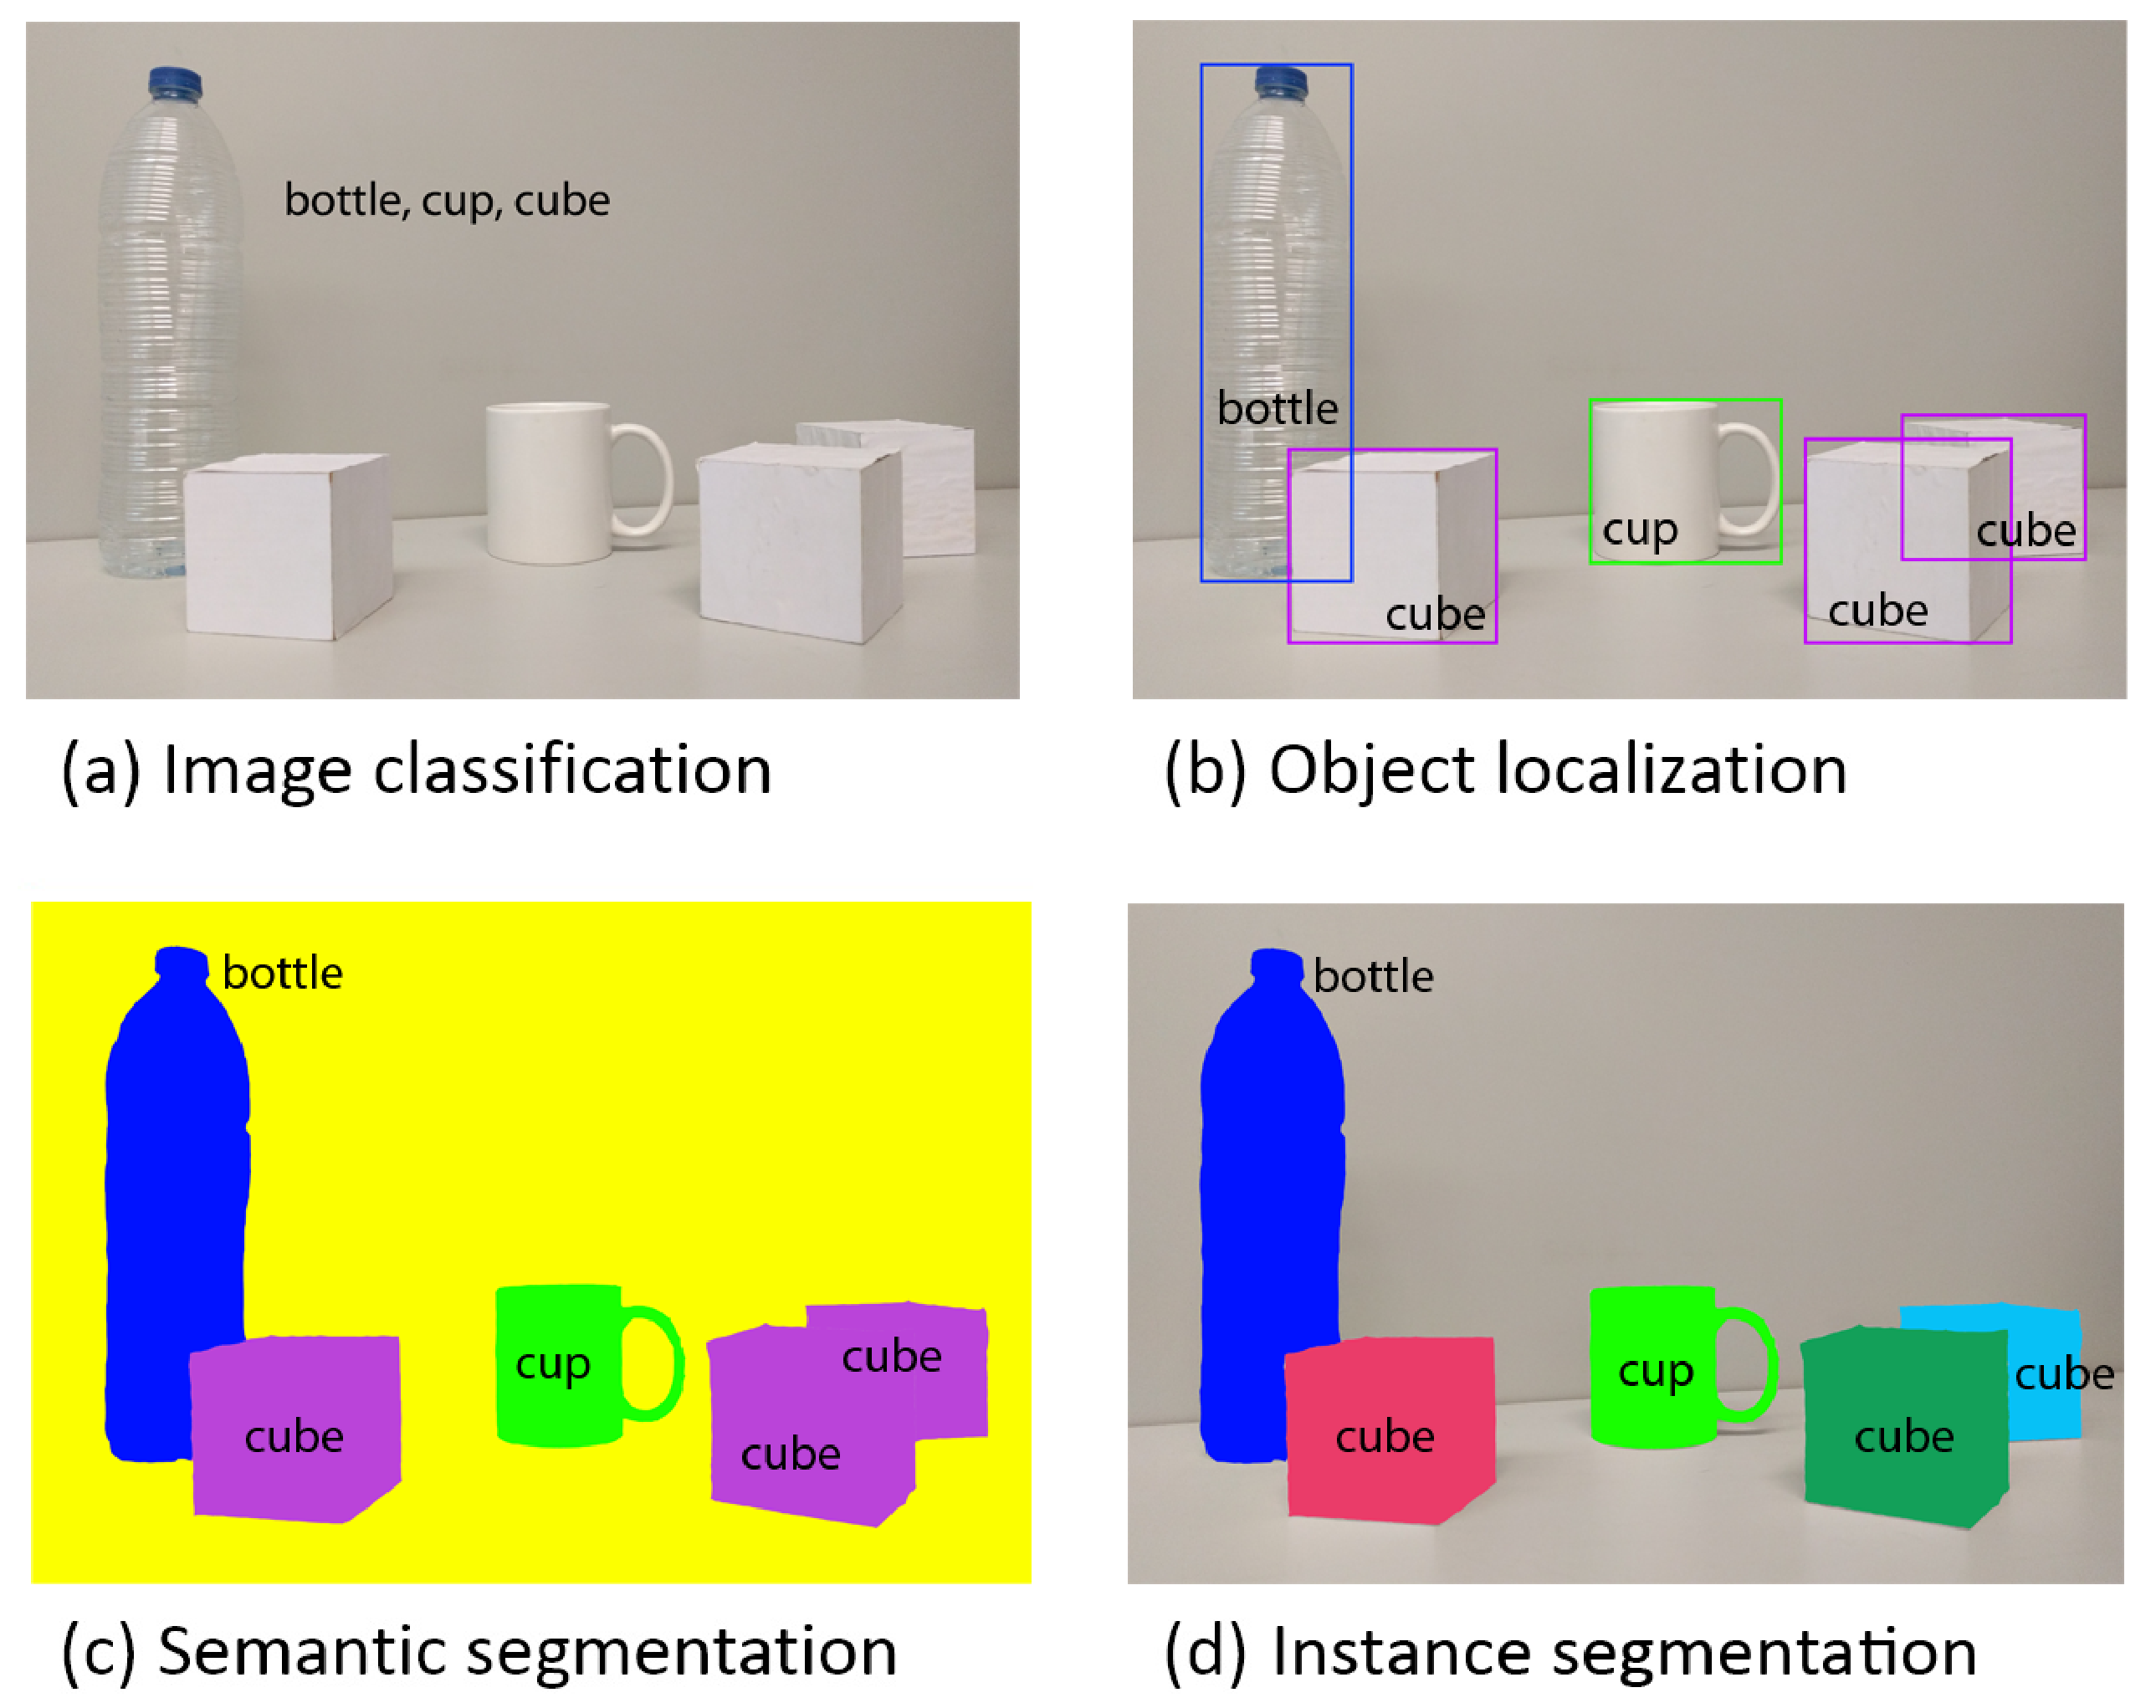
\includegraphics[width=0.8\linewidth]{Figures/Segmentation/example_rework.eps}
	\caption{Evolution of object recognition or scene understanding from coarse-grained to fine-grained inference: classification, detection or localization, semantic segmentation, and instance segmentation.}
	\label{fig:background_evolution}
\end{figure}

To the best of our knowledge, this is the first review to focus explicitly on deep learning for semantic segmentation. Various semantic segmentation surveys already exist such as the works by Zhu \emph{et al.}\cite{Zhu2016} and Thoma\cite{Thoma2016}, which do a great work summarizing and classifying existing methods, discussing datasets and metrics, and providing design choices for future research directions. However, they lack some of the most recent datasets, they do not analyze frameworks, and none of them provide details about deep learning techniques. Because of that, we consider our work to be novel and helpful thus making it a significant contribution for the research community.

The key contributions of our work are as follows:

\begin{itemize}
	\item We provide a broad survey of existing datasets that might be useful for segmentation projects with deep learning techniques.
	\item An in-depth and organized review of the most significant methods that use deep learning for semantic segmentation, their origins, and their contributions.
	\item A thorough performance evaluation which gathers quantitative metrics such as accuracy, execution time, and memory footprint.
	\item A discussion about the aforementioned results, as well as a list of possible future works that might set the course of upcoming advances, and a conclusion summarizing the state of the art of the field.
\end{itemize}

The remainder of this chapter is organized as follows. Firstly, Section \ref{cha:semseg:sec:background} introduces the semantic segmentation problem as well as notation and conventions commonly used in the literature and background concepts. Next, Section \ref{cha:semseg:sec:datasets} describes existing datasets, challenges, and benchmarks. Section \ref{cha:semseg:sec:methods} reviews existing methods. Finally, Section \ref{cha:semseg:sec:discussion} presents a brief discussion on the presented methods based on their quantitative results on the aforementioned datasets. In addition, future research directions are also laid out. At last, Section \ref{cha:semseg:sec:conclusion} summarizes the chapter and draws conclusions about this work and the state of the art of the field.

\section{Terminology and Background Concepts}
\label{cha:semseg:sec:background}

In order to properly understand how semantic segmentation is tackled by modern deep learning architectures, it is important to know that it is not an isolated field but rather a natural step in the progression from coarse to fine inference. The origin could be located at classification, which consists of making a prediction for a whole input, i.e., predicting which is the object in an image or even providing a ranked list if there are many of them. Localization or detection is the next step towards fine-grained inference, providing not only the classes but also additional information regarding the spatial location of those classes, e.g., centroids or bounding boxes. Providing that, it is obvious that semantic segmentation is the natural step to achieve fine-grained inference, its goal: make dense predictions inferring labels for every pixel; this way, each pixel is labeled with the class of its enclosing object or region. Further improvements can be made, such as instance segmentation (separate labels for different instances of the same class) and even part-based segmentation (low-level decomposition of already segmented classes into their components). Figure \ref{fig:background_evolution} shows the aforementioned evolution. In this review, we will mainly focus on generic scene labeling, i.e., per-pixel class segmentation, but we will also review the most important methods on instance and part-based segmentation.

In the end, the per-pixel labeling problem can be reduced to the following formulation: find a way to assign a state from the label space $\mathcal{L} = \{l_1, l_2, ... , l_k\}$ to each one of the elements of a set of random variables $\mathcal{X} = \{x_1, x_2, ... , x_N\}$. Each label $l$ represents a different class or object, e.g., aeroplane, car, traffic sign, or background. This label space has $k$ possible states which are usually extended to $k+1$ and treating $l_0$ as background or a void class. Usually, $\mathcal{X}$ is a \acs{2D} image of $W\times H = N$ pixels $x$. However, that set of random variables can be extended to any dimensionality such as volumetric data or hyperspectral images.

Apart from the problem formulation, it is important to remark some background concepts that might help the reader to understand this review. Firstly, common networks, approaches, and design decisions that are often used as the basis for deep semantic segmentation systems. In addition, common techniques for training such as transfer learning. At last, data pre-processing and augmentation approaches.

\subsection{Common Deep Network Architectures}

As we previously stated, certain deep networks have made such significant contributions to the field that they have become widely known standards. It is the case of AlexNet, \acs{VGG}-16, GoogLeNet, and ResNet. Such was their importance that they are currently being used as building blocks for many segmentation architectures. We will devote this section to review them.

\subsubsection{AlexNet}

AlexNet was the pioneering deep \acs{CNN} that won the \acs{ILSVRC}-2012 with a TOP-5 test accuracy of $84.6\%$ while the closest competitor, which made use of traditional techniques instead of deep architectures, achieved a $73.8\%$ accuracy in the same challenge. The architecture presented by Krizhevsky \emph{et al.} \cite{Krizhevsky2012} was relatively simple:five convolutional layers, max-pooling ones, \acp{ReLU} as non-linearities, three fully-connected layers, and dropout (see Figure \ref{fig:semseg:alexnet}).

\begin{figure}[!hbt]
	\centering
	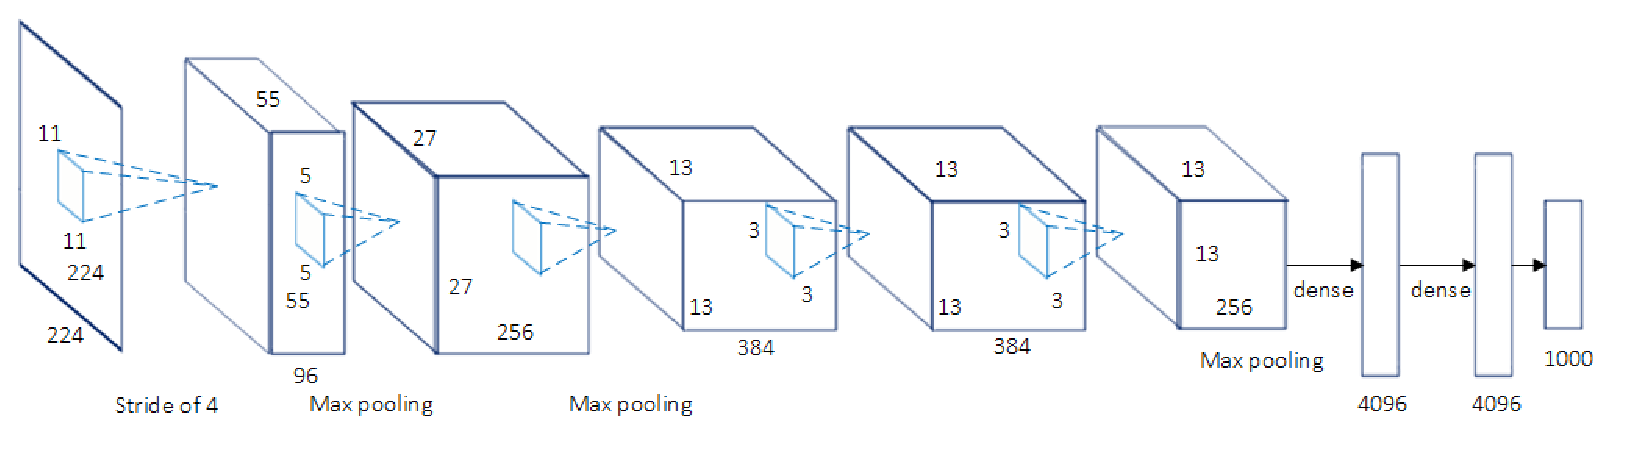
\includegraphics[width=0.9\linewidth]{Figures/Segmentation/alexnet_rework.eps}
	\caption{AlexNet \acl{CNN} architecture. Figure reproduced from \cite{Krizhevsky2012}.}
	\label{fig:semseg:alexnet}
\end{figure}

\subsubsection{\acs{VGG}}

\acs{VGG} is a \ac{CNN} model introduced by the \acf{VGG} from the University of Oxford. They proposed various models and configurations of deep \acp{CNN} \cite{Simonyan2014}, one of them was submitted to the \ac{ILSVRC}-2013. That model, also known as \acs{VGG}-16 due to the fact that it is composed by $16$ weight layers, became popular thanks to its achievement of $92.7\%$ TOP-5 test accuracy. Figure \ref{fig:segmentation:vgg16} shows the configuration of \acs{VGG}-16. The main difference between \acs{VGG}-16 and its predecessors is the use of a stack of convolution layers with small receptive fields in the first layers instead of few layers with big receptive fields. This leads to less parameters and more non-linearities in between, thus making the decision function more discriminative and the model easier to train.

\begin{figure}[!hbt]
	\centering
	\includegraphics[width=0.8\linewidth]{Figures/Segmentation/vgg16.eps}
    \caption{\acs{VGG}-16 \acs{CNN} architecture. Figure extracted from \cite{Noh2015}.}
	\label{fig:segmentation:vgg16}
\end{figure}

\subsubsection{GoogLeNet}

GoogLeNet is a network introduced by Szegedy \emph{et al.} \cite{Szegedy2015} which won the \ac{ILSVRC}-2014 challenge with a TOP-5 test accuracy of $93.3\%$. This \acs{CNN} architecture is characterized by its complexity, emphasized by the fact that it is composed by $22$ layers and a newly introduced building block called \emph{inception} module (see Figure \ref{fig:segmentation:inception-module}). This new approach proved that \acs{CNN} layers could be stacked in more ways than a typical sequential manner. In fact, those modules consist of a \ac{NiN} layer, a pooling operation, a large-sized convolution layer, and small-sized convolution layer. All of them are computed in parallel and followed by $1\times1$ convolution operations to reduce dimensionality. Thanks to those modules, this network puts special consideration on memory and computational cost by significantly reducing the number of parameters and operations.

\begin{figure}[!hbt]
\centering
 \scalebox{.7}
 {
	\begin{tikzpicture}[auto, >=latex']
	\node [block, fill=white] (filterconcat) [align=center] {Filter\\concatenation};
	\node [block, fill=cyan!35, below left of= filterconcat, node distance = 6em] (3x3conv) {3x3 convolutions};
	\node [block, fill=cyan!70, below right of= filterconcat, node distance = 6em] (5x5conv) {5x5 convolutions} ;
	\node [block, fill=cyan!15, left of = 3x3conv, node distance= 10em] (1x1conv0) {1x1 convolutions};
	\node [block, fill=cyan!15, right of= 5x5conv, node distance= 10em] (1x1conv1) {1x1 convolutions};
	\node [block, fill=cyan!15, below of= 3x3conv, node distance=4 em] (1x1conv2) {1x1 convolutions};
	\node [block, fill=cyan!15, below of= 5x5conv, node distance=4 em] (1x1conv3) {1x1 convolutions};
	\node [block, fill=red!40, below of= 1x1conv1, node distance= 4em] (3x3max) {3x3 max pooling};
	\node [block, fill=white, below left of= 1x1conv3, node distance=6em] (prevlayer) {Previous layer};
		
	\draw[edge] (3x3conv.north) |- (filterconcat.west);
	\draw[edge] (1x1conv0.north) |- (filterconcat.west);
	\draw[edge] (5x5conv.north) |- (filterconcat.east);
	\draw[edge] (1x1conv1.north) |- (filterconcat.east);
	\draw[edge] (1x1conv2.north) -- (3x3conv.south);
	\draw[edge] (1x1conv3.north) -- (5x5conv.south);
	\draw[edge] (3x3max.north) -- (1x1conv1.south);
	\draw[edge] (prevlayer) -| (1x1conv0.south);
	\draw[edge] (prevlayer) -| (1x1conv2.south);
	\draw[edge] (prevlayer) -| (1x1conv3.south);
	\draw[edge] (prevlayer) -| (3x3max.south);
	\end{tikzpicture}
}
	\caption{Inception module with dimensionality reduction from the GoogLeNet architecture. Figure reproduced from \cite{Szegedy2015}.}
	\label{fig:segmentation:inception-module}
\end{figure}


\subsubsection{ResNet}

Microsoft's ResNet\cite{He2016} is specially remarkable thanks to winning \ac{ILSVRC}-2016 with $96.4\%$ accuracy. Apart from that fact, the network is well-known due to its depth ($152$ layers) and the introduction of residual blocks (see Figure \ref{fig:segmentation:resnet-block}). The residual blocks address the problem of training a really deep architecture by introducing identity skip connections so that layers can copy their inputs to the next layer.

\begin{figure}[!hbt]
	\centering
	\begin{tikzpicture}[auto, node distance=1.8 cm,>=latex']
	\node [input, name=input] {};
	\node [block, fill=cyan!20, below of= input] (weightlayer1) {weight layer};
	\node [block, fill=cyan!20, below of= weightlayer1] (weightlayer2) {weight layer};
	\node [sum, below of= weightlayer2, label={[xshift=-1.2cm, yshift= -0.55cm] $F(\chi) + \chi$}] (sum) {+};
	\coordinate[right of= sum] (midpoint) {};
	
	
	\draw[draw, ->] (input) [left] -- node [name=inputedge] {$\chi$} (weightlayer1);
	\draw[->] (weightlayer1) [left] -- node [xshift=-1cm] {$F(\chi)$} (weightlayer2);
	\draw[->] (weightlayer2) -- (sum);
	\draw[-] (inputedge) -| node [yshift=-2cm, align=center] {$\chi$\\identity}(midpoint);
	\draw[->] (midpoint) -- node {$relu$} (sum.east);
	\end{tikzpicture}
	\caption{Residual block from ResNet. Figure reproduced from \cite{He2016}.}
	\label{fig:segmentation:resnet-block}
\end{figure}

The intuitive idea behind this approach is that it ensures that the next layer learns something new and different from what the input has already encoded (since it is provided with both the output of the previous layer and its unchanged input). In addition, this kind of connections help overcoming the vanishing gradients problem.

\subsubsection{ReNet}

In order to extend \acp{RNN} architectures to multi-dimensional tasks, Graves et al. \cite{Graves2007} proposed a \ac{MDRNN} architecture which replaces each single recurrent connection from standard \acsp{RNN} with $d$ connections, where $d$ is the number of spatio-temporal data dimensions. Based on this initial approach, Visin el al. \cite{Visin2015} proposed ReNet architecture in which instead of multidimensional \acsp{RNN}, they have been using usual sequence \acsp{RNN}. In this way, the number of \acsp{RNN} is scaling linearly at each layer regarding to the number of dimensions $d$ of the input image ($2d$). In this approach, each convolutional layer (convolution + pooling) is replaced with four \acsp{RNN} sweeping the image vertically and horizontally in both directions as we can see in Figure \ref{fig:segmentation:renet}.

\begin{figure}[!hbt]
	\centering
	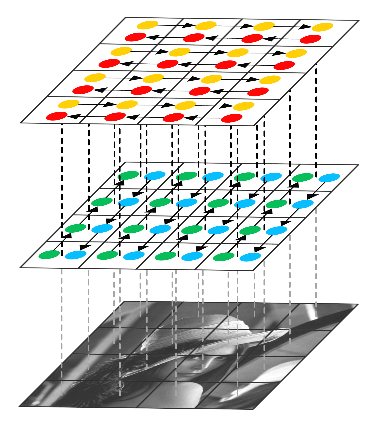
\includegraphics[width=0.5\linewidth]{Figures/Segmentation/renet_rework.eps}
	\caption{One layer of ReNet architecture modeling vertical and horizontal spatial dependencies. Extracted from \cite{Visin2015}.}
	\label{fig:segmentation:renet}
\end{figure}

\subsection{Transfer Learning and Fine-tuning}

Training a deep neural network from scratch is often not feasible because of various reasons: a dataset of sufficient size is required (and not usually available) and reaching convergence can take too long for the experiments to be worth. Even if a dataset large enough is available and convergence does not take that long, it is often helpful to start with pre-trained weights instead of random initialized ones\cite{Ahmed2008}\cite{Oquab2014}. Fine-tuning the weights of a pre-trained network by continuing with the training process is one of the major transfer learning scenarios.

Yosinski \emph{et al.}\cite{Yosinski2014} proved that transferring features even from distant tasks can be better than using random initialization, taking into account that the transferability of features decreases as the difference between the pre-trained task and the target one increases.

However, applying this transfer learning technique is not completely straightforward. On the one hand, there are architectural constraints that must be met to use a pre-trained network. Nevertheless, since it is not usual to come up with a whole new architecture, it is common to reuse already existing network architectures (or components) thus enabling transfer learning. On the other hand, the training process differs slightly when fine-tuning instead of training from scratch. It is important to choose properly which layers to fine-tune -- usually the higher-level part of the network, since the lower one tends to contain more generic features -- and also pick an appropriate policy for the learning rate, which is usually smaller due to the fact that the pre-trained weights are expected to be relatively good so there is no need to drastically change them.

Transfer learning from ImageNet pre-trained networks is common for semantic segmentation. Nevertheless, the interest in modeling representations using self-supervised, weakly-supervised and unsupervised learning increasingly predominates. Pre-trained weights of context encoders used for context-based pixel prediction aiming semantic hole-filling, have been used for initializing a \acs{FCN} \cite{Pathak2016}. This setting outperform random initialized networks and plain autoencoders thus advancing the state of the art in semantic segmentation.

Due to the inherent difficulty of gathering and creating per-pixel labelled segmentation datasets, their scale is not as large as the size of classification datasets such as ImageNet\cite{Deng2009}\cite{Russakovsky2015}. This problem gets even worse when dealing with \acs{RGB-D} or \acs{3D} datasets, which are even smaller. For that reason, transfer learning, and in particular fine-tuning from pre-trained classification networks is a common trend for segmentation networks and has been successfully applied in the methods that we will review in the following sections.Although the datasets are smaller the more detailed the semantic labelling, a feasible solution to this problem is the use of synthetic datasets extracted from commercial video games. Some experiments on semantic segmentation shows that models trained with game data and $\frac{1}{3}$ of the CamVid dataset outperform methods trained on the complete CamVid training set \cite{Richter2016}. This technique relies on a two-staged process: (1) real and synthetic data are used jointly to train the model, (2) model will be fine-tunned with only real data.

Due to the inherent difficulty of gathering and creating per-pixel labelled segmentation datasets, their scale is not as large as the size of classification datasets such as ImageNet\cite{Deng2009}\cite{Russakovsky2015}. This problem gets even worse when dealing with \acs{RGB-D} or \acs{3D} datasets, which are even smaller. For that reason, transfer learning, and in particular fine-tuning from pre-trained classification networks is a common trend for segmentation networks and has been successfully applied in the methods that we will review in the following sections.

\subsection{Data Preprocessing and Augmentation}

Data augmentation is a common technique that has been proven to benefit the training of machine learning models in general and deep architectures in particular; either speeding up convergence or acting as a regularizer, thus avoiding overfitting and increasing generalization capabilities\cite{Wong2016}.

It typically consist of applying a set of transformations in either data or feature spaces, or even both. The most common augmentations are performed in the data space. That kind of augmentation generates new samples by applying transformations to the already existing data. There are many transformations that can be applied: translation, rotation, warping, scaling, color space shifts, crops, etc. The goal of those transformations is to generate more samples to create a larger dataset, preventing overfitting and presumably regularizing the model, balance the classes within that database, and even synthetically produce new samples that are more representative for the use case or task at hand.

Augmentations are specially helpful for small datasets, and have proven their efficacy with a long track of success stories. For instance, in \cite{Shen2016}, a dataset of $1500$ portrait images is augmented synthesizing four new scales ($0.6, 0.8, 1.2, 1.5$), four new rotations ($-45, -22, 22, 45$), and four gamma variations ($0.5, 0.8, 1.2, 1.5$) to generate a new dataset of $19000$ training images. That process allowed them to raise the accuracy of their system for portrait segmentation from $73.09$ to $94.20$ \ac{IoU} when including that augmented dataset for fine-tuning.

\section{Datasets}
\label{cha:semseg:sec:datasets}

In this section we present the main content of this paper: an in-depth review of existing datasets and methods together with an evaluation of their quality, relevance, and impact in the field. Both of them are presented according to a well thought taxonomy of the research completed in the area.

Datasets were sampled from a wide variety of application scenarios and subdivided according to their data representation (2D, 2.5D, or 3D) since that is the first factor to take into account when choosing a dataset. Apart from that we categorize them according to other application-specific factors which are later described in detail. The datasets were selected mainly by using a criteria of relevance (popularity by means of citation reports, usage as benchmarking tools, and scientific quality enforced by top-tier venues and journals) and usefulness for the community (novel data or application scenarios). We also focused on taking into account their scale and possibilities for training deep architectures.

The same criteria of relevance was applied when selecting methods. Certain outdated methods were still selected for completeness when describing improved versions of those or even newer ones. Others were also included due to their importance in laying the fundamentals for future research. The rest of the methods were selected due to the impact of their main contributions either by creating a new research direction (e.g., instance segmentation, sequence processing, 3D segmentation) or  pushing forward the limits of a certain aspect (e.g., accuracy, efficiency, or training capabilities). More details about the followed taxonomy can be found later in the corresponding section.

Two kinds of readers are expected for this type of review: either they are initiating themselves in the problem, or either they are experienced enough and they are just looking for the most recent advances made by other researchers in the last few years. Although the second kind is usually aware of two of the most important aspects to know before starting to research in this problem, it is critical for newcomers to get a grasp of what are the top-quality datasets and challenges. Therefore, the purpose of this section is to help novel scientists get to speed, providing them with a brief summary of datasets that might suit their needs as well as  data augmentation and preprocessing tips. Nevertheless, it can also be useful for hardened researchers who want to review the fundamentals or maybe discover new information. 

In the following lines we describe the most popular large-scale datasets currently in use for semantic segmentation. All datasets listed here provide appropriate pixel-wise or point-wise labels. The list is structured into three parts according to the nature of the data: \acs{2D} or plain \acs{RGB} datasets, \acs{2.5D} or \ac{RGB-D} ones, and pure volumetric or \acs{3D} databases. Table \ref{table:datasets} shows a summarized view, gathering all the described datasets and providing useful information such as their purpose, number of classes, data format, and training/validation/testing splits.

\begin{table*}[!t]
	\centering
	\caption{Popular large-scale segmentation datasets.}
	\resizebox{\linewidth}{!}{
	\begin{tabular}{|c|c|c|c|c|c|c|c|c|c|c|}
		\hline
		Name and Reference & Purpose & Year & Classes & Data & Resolution & Sequence & Synthetic/Real & Samples (training) & Samples (validation) & Samples (test)\\
		\hline
		PASCAL \acs{VOC} 2012 Segmentation \cite{Everingham2015} & Generic & 2012 & 21 & 2D & Variable & \xmark & R & $1464$ & $1449$ & Private\\
		PASCAL-Context \cite{Mottaghi2014} & Generic & 2014 & 540 (59) & 2D & Variable & \xmark & R & $10103$ & N/A & $9637$\\
		PASCAL-Part \cite{Chen2014} & Generic-Part & 2014 & 20 & 2D & Variable & \xmark & R & $10103$ & N/A & $9637$\\
		\acs{SBD} \cite{Hariharan2011} & Generic & 2011 & 21 & 2D & Variable & \xmark & R & $8498$ & $2857$ & N/A\\
		Microsoft \acs{COCO} \cite{Lin2014} & Generic & 2014 & +80 & 2D & Variable & \xmark & R & $82783$ & $40504$ & $81434$\\
		\acs{SYNTHIA} \cite{Ros2016} & Urban (Driving)& 2016 & 11 & 2D & $960\times720$ & \xmark & S & $13407$ & N/A & N/A\\
		Cityscapes (fine) \cite{Cordts2015} & Urban & 2015 &30 (8) & 2D & $2048\times1024$ & \cmark & R & $2975$ & $500$ & $1525$\\
		Cityscapes (coarse) \cite{Cordts2015} & Urban & 2015 & 30 (8) & 2D & $2048\times1024$ & \cmark & R & $22973$ & $500$ & N/A\\
		CamVid \cite{Brostow2009} & Urban (Driving) & 2009 & 32 & 2D & $960\times720$ & \cmark & R & $701$ & N/A & N/A\\
		CamVid-Sturgess \cite{Sturgess2009} & Urban (Driving) & 2009 & 11 & 2D & $960\times720$ & \cmark & R & $367$ & $100$ & $233$\\
		KITTI-Layout \cite{Alvarez2012}\cite{Ros2015a} & Urban/Driving & 2012 & 3 & 2D & Variable & \xmark & R & $323$ & N/A & N/A\\
		KITTI-Ros \cite{Ros2015} & Urban/Driving & 2015 & 11 & 2D & Variable & \xmark & R & $170$ & N/A & $46$\\
		KITTI-Zhang \cite{Zhang2015} & Urban/Driving & 2015 & 10 & 2D/3D & $1226\times370$ & \xmark & R & $140$ & N/A & $112$\\
		Stanford background \cite{Gould2009} & Outdoor & 2009 & 8 & 2D & $320\times240$ & \xmark & R & $725$ & N/A & N/A\\
		SiftFlow \cite{Liu2009} & Outdoor & 2011 & 33 & 2D & $256\times256$ & \xmark  & R & $2688$ & N/A & N/A \\
		Youtube-Objects-Jain \cite{Jain2014} & Objects & 2014 & 10 & 2D & $480\times360$ & \cmark & R & $10167$ & N/A & N/A\\
		Adobe's Portrait Segmentation \cite{Shen2016} & Portrait & 2016 & 2 & 2D & $600\times800$ & \xmark & R & $1500$ & $300$ & N/A\\
		\acs{MINC} \cite{Bell2015} & Materials & 2015 & 23 & 2D & Variable & \xmark & R & $7061$ & $2500$ & $5000$\\
		\acs{DAVIS} \cite{Perazzi2016}\cite{Pont-Tuset2017} & Generic & 2016 & 4 & 2D & 480p & \cmark & R & $4219$ & $2023$ & $2180$\\
		NYUDv2 \cite{Silberman2012} & Indoor & 2012 & 40 & 2.5D & $480\times640$ & \xmark & R & $795$ & $654$ & N/A\\
%		Berkeley B3DO \cite{Janoch2013} & ??? & ??? & 2.5D & ??? & ??? & ??? & ??? & ???\\
		SUN3D \cite{Xiao2013} & Indoor & 2013 & -- & 2.5D & $640\times480$ & \cmark & R & $19640$ & N/A & N/A\\
		SUNRGBD \cite{Song2015b} & Indoor & 2015 & 37 & 2.5D & Variable & \xmark & R & $2666$ & $2619$ & $5050$\\
%		The Object Segmentation Database (OSD) \cite{richtsfeld2012object} & Object & ??? & 2.5D & ??? & ??? & 45 & N/A & 66\\
		RGB-D Object Dataset\cite{lai2011large} & Household objects & 2011 & 51 & 2.5D & $640\times480$ & \cmark & R & $207920$ & N/A & N/A\\
		ShapeNet Part\cite{Yi2016} & Object/Part & 2016 & 16/50 & 3D & N/A & \xmark & S & $31,963$ & N/A & N/A\\
		Stanford 2D-3D-S\cite{Armeni2017} & Indoor & 2017 & 13 & 2D/2.5D/3D & $1080\times1080$ & \cmark & R & $70469$ & N/A & N/A\\
		3D Mesh \cite{Chen:2009:ABF} & Object/Part & 2009 & 19 & 3D & N/A & \xmark & S & 380 & N/A & N/A\\
		Sydney Urban Objects Dataset\cite{quadros2012feature} & Urban (Objects) & 2013 & 26 & 3D & N/A & \xmark & R & $41$ & N/A & N/A\\
		%3D Segmentation Benchmark\cite{benhabiles2009framework} & ??? & ??? & 3D & N/A & \xmark & 28 & N/A & N/A\\
		Large-Scale Point Cloud Classification Benchmark\cite{hackel2016contour} & Urban/Nature & 2016 & 8 & 3D & N/A & \xmark  &  R & $15$ & N/A & $15$\\
		
		\hline
	\end{tabular}}
	\label{table:datasets}
\end{table*}

\subsection{2D Datasets}

Throughout the years, semantic segmentation has been mostly focused on \acl{2D} images. For that reason, \acs{2D} datasets are the most abundant ones. In this section we describe the most popular \acs{2D} large-scale datasets for semantic segmentation, considering \acs{2D} any dataset that contains any kind of \acl{2D} representations such as gray-scale or \ac{RGB} images.

\begin{itemize}
	\item \textbf{PASCAL \acf{VOC}}\cite{Everingham2015}\footnote{\url{http://host.robots.ox.ac.uk/pascal/VOC/voc2012/}}: this challenge consists of a ground-truth annotated dataset of images and five different competitions: classification, detection, segmentation, action classification, and person layout. The segmentation one is specially interesting since its goal is to predict the object class of each pixel for each test image. There are 21 classes categorized into vehicles, household, animals, and other: aeroplane, bicycle, boat, bus, car, motorbike, train, bottle, chair, dining table, potted plant, sofa, TV/monitor, bird, cat, cow, dog, horse, sheep, and person. Background is also considered if the pixel does not belong to any of those classes. The dataset is divided into two subsets: training and validation with 1464 and 1449 images respectively. The test set is private for the challenge. This dataset is arguably the most popular for semantic segmentation so almost every remarkable method in the literature is being submitted to its performance evaluation server to validate against their private test set. Methods can be trained either using only the dataset or either using additional information. Furthermore, its leaderboard is public and can be consulted online\footnote{\url{http://host.robots.ox.ac.uk:8080/leaderboard/displaylb.php?challengeid=11&compid=6}}.
	\item \textbf{PASCAL Context}\cite{Mottaghi2014}\footnote{\url{http://www.cs.stanford.edu/~roozbeh/pascal-context/}}: this dataset is an extension of the PASCAL \ac{VOC} 2010 detection challenge which contains pixel-wise labels for all training images ($10103$). It contains a total of $540$ classes -- including the original 20 classes plus background from PASCAL \ac{VOC} segmentation -- divided into three categories (objects, stuff, and hybrids). Despite the large number of categories, only the 59 most frequent are remarkable. Since its classes follow a power law distribution, there are many of them which are too sparse throughout the dataset. In this regard, this subset of 59 classes is usually selected to conduct studies on this dataset, relabeling the rest of them as background.
	\item \textbf{PASCAL Part}\cite{Chen2014}\footnote{\url{http://www.stat.ucla.edu/~xianjie.chen/pascal_part_dataset/pascal_part.html}}: this database is an extension of the PASCAL \ac{VOC} 2010 detection challenge which goes beyond that task to provide per-pixel segmentation masks for each part of the objects (or at least silhouette annotation if the object does not have a consistent set of parts). The original classes of PASCAL \ac{VOC} are kept, but their parts are introduced, e.g., bicycle is now decomposed into back wheel, chain wheel, front wheel, handlebar, headlight, and saddle. It contains labels for all training and validation images from PASCAL \ac{VOC} as well as for the 9637 testing images.
	\item \textbf{\acf{SBD}}\cite{Hariharan2011}\footnote{\url{http://home.bharathh.info/home/sbd}}: this dataset is an extended version of the aforementioned PASCAL \ac{VOC} which provides semantic segmentation ground truth for those images that were not labelled in \ac{VOC}. It contains annotations for $11355$ images from PASCAL \ac{VOC} $2011$. Those annotations provide both category-level and instance-level information, apart from boundaries for each object. Since the images are obtained from the whole PASCAL \ac{VOC} challenge (not only from the segmentation one), the training and validation splits diverge. In fact, \ac{SBD} provides its own training ($8498$ images) and validation ($2857$ images) splits. Due to its increased amount of training data, this dataset is often used as a substitute for PASCAL \ac{VOC} for deep learning.
	\item \textbf{Microsoft \acf{COCO}}\cite{Lin2014}\footnote{\url{http://mscoco.org/}}: is another image recognition, segmentation, and captioning large-scale dataset. It features various challenges, being the detection one the most relevant for this field since one of its parts is focused on segmentation. That challenge, which features more than $80$ classes, provides more than $82783$ images for training, $40504$ for validation, and its test set consist of more than $80000$ images. In particular, the test set is divided into four different subsets or splits: test-dev ($20000$ images) for additional validation, debugging, test-standard ($20000$ images) is the default test data for the competition and the one used to compare state-of-the-art methods, test-challenge ($20000$ images) is the split used for the challenge when submitting to the evaluation server, and test-reserve ($20000$ images) is a split used to protect against possible overfitting in the challenge (if a method is suspected to have made too many submissions or trained on the test data, its results will be compared with the reserve split). Its popularity and importance has ramped up since its appearance thanks to its large scale. In fact, the results of the challenge are presented yearly on a joint workshop at the \ac{ECCV}\footnote{\url{http://image-net.org/challenges/ilsvrc+coco2016}} together with ImageNet's ones.
	\item \textbf{\ac{SYNTHIA}}\cite{Ros2016}\footnote{\url{http://synthia-dataset.net/}}: is a large-scale collection of photo-realistic renderings of a virtual city, semantically segmented, whose purpose is scene understanding in the context of driving or urban scenarios.The dataset provides fine-grained pixel-level annotations for $11$ classes (void, sky, building, road, sidewalk, fence, vegetation, pole, car, sign, pedestrian, and cyclist). It features $13407$ training images from rendered video streams. It is also characterized by its diversity in terms of scenes (towns, cities, highways), dynamic objects, seasons, and weather.
	\item \textbf{Cityscapes}\cite{Cordts2015}\footnote{\url{https://www.cityscapes-dataset.com/}}: is a large-scale database which focuses on semantic understanding of urban street scenes. It provides semantic, instance-wise, and dense pixel annotations for 30 classes grouped into 8 categories (flat surfaces, humans, vehicles, constructions, objects, nature, sky, and void). The dataset consist of around 5000 fine annotated images and 20000 coarse annotated ones. Data was captured in 50 cities during several months, daytimes, and good weather conditions. It was originally recorded as video so the frames were manually selected to have the following features: large number of dynamic objects, varying scene layout, and varying background.
	\item \textbf{CamVid}\cite{Brostow2008}\cite{Brostow2009}\footnote{\url{http://mi.eng.cam.ac.uk/research/projects/VideoRec/CamVid/}}: is a road/driving scene understanding database which was originally captured as five video sequences with a $960\times720$ resolution camera mounted on the dashboard of a car. Those sequences were sampled (four of them at 1 fps and one at 15 fps) adding up to $701$ frames. Those stills were manually annotated with $32$ classes: void, building, wall, tree, vegetation, fence, sidewalk, parking block, column/pole, traffic cone, bridge, sign, miscellaneous text, traffic light, sky, tunnel, archway, road, road shoulder, lane markings (driving), lane markings (non-driving), animal, pedestrian, child, cart luggage, bicyclist, motorcycle, car, SUV/pickup/truck, truck/bus, train, and other moving object. It is important to remark the partition introduced by Sturgess \emph{et al.}\cite{Sturgess2009} which divided the dataset into $367/100/233$ training, validation, and testing images respectively. That partition makes use of a subset of class labels: building, tree, sky, car, sign, road, pedestrian, fence, pole, sidewalk, and bicyclist.
	\item \textbf{KITTI}\cite{Geiger2013}: is one of the most popular datasets for use in mobile robotics and autonomous driving. It consists of hours of traffic scenarios recorded with a variety of sensor modalities, including high-resolution RGB, grayscale stereo cameras, and a 3D laser scanner. Despite its popularity, the dataset itself does not contain ground truth for semantic segmentation. However, various researchers have manually annotated parts of the dataset to fit their necessities. Álvarez \emph{et al.}\cite{Alvarez2012}\cite{Ros2015a} generated ground truth for $323$ images from the road detection challenge with three classes: road, vertical, and sky. Zhang \emph{et al.}\cite{Zhang2015} annotated $252$ ($140$ for training and $112$ for testing) acquisitions -- RGB and Velodyne scans -- from the tracking challenge for ten object categories: building, sky, road, vegetation, sidewalk, car, pedestrian, cyclist, sign/pole, and fence. Ros \emph{et al.} \cite{Ros2015} labeled $170$ training images and $46$ testing images (from the visual odometry challenge) with $11$ classes: building, tree, sky, car, sign, road, pedestrian, fence, pole, sidewalk, and bicyclist.
	\item \textbf{Youtube-Objects}\cite{Prest2012} is a database of videos collected from YouTube which contain objects from ten PASCAL \acs{VOC} classes: aeroplane, bird, boat, car, cat, cow, dog, horse, motorbike, and train. That database  does not contain pixel-wise annotations but Jain \emph{et al.}\cite{Jain2014} manually annotated a subset of $126$ sequences. They took every 10th frame from those sequences and generated semantic labels. That totals  $10167$ annotated frames at $480\times360$ pixels resolution.
	\item \textbf{Adobe's Portrait Segmentation}\cite{Shen2016}\footnote{\url{http://xiaoyongshen.me/webpage_portrait/index.html}}: this is a dataset of $800\times600$ pixels portrait images collected from Flickr, mainly captured with mobile front-facing cameras. The database consist of $1500$ training images and $300$ reserved for testing, both sets are fully binary annotated: person or background. The images were labeled in a semi-automatic way: first a face detector was run on each image to crop them to $600\times800$ pixels and then persons were manually annotated using Photoshop quick selection. This dataset is remarkable due to its specific purpose which makes it suitable for person in foreground segmentation applications.
	\item \textbf{\ac{MINC}}\cite{Bell2015}: this work is a dataset for patch material classification and full scene material segmentation. The dataset provides segment annotations for $23$ categories: wood, painted, fabric, glass, metal, tile, sky, foliage, polished stone, carpet, leather, mirror, brick, water, other, plastic, skin, stone, ceramic, hair, food, paper, and wallpaper. It contains $7061$ labeled material segmentations for training, $5000$ for test, and $2500$ for validation. The main source for these images is the OpenSurfaces dataset \cite{Bell2013}, which was augmented using other sources of imagery such as Flickr or Houzz. For that reason, image resolution for this dataset varies. On average, image resolution is approximately  $800\times500$ or $500\times800$.
	\item \textbf{\ac{DAVIS}}\cite{Perazzi2016}\cite{Pont-Tuset2017}\footnote{\url{http://davischallenge.org/index.html}}: this challenge is purposed for video object segmentation. Its dataset is composed by $50$ high-definition sequences which add up to $4219$ and $2023$ frames for training and validation respectively. Frame resolution varies across sequences but all of them were downsampled to $480$p for the challenge. Pixel-wise annotations are provided for each frame for four different categories: human, animal, vehicle, and object. Another feature from this dataset is the presence of at least one target foreground object in each sequence. In addition, it is designed not to have many different objects with significant motion. For those scenes which do have more than one target foreground object from the same class, they provide separated ground truth for each one of them to allow instance segmentation.
	\item \textbf{Stanford background}\cite{Gould2009}\footnote{\url{http://dags.stanford.edu/data/iccv09Data.tar.gz}}: dataset with outdoor scene images imported from existing public datasets: LabelMe, MSRC, PASCAL VOC and Geometric Context. The dataset contains 715 images (size of $320\times240$ pixels)  with at least one foreground object and having the horizon position within the image. The dataset is pixel-wise annotated (horizon location, pixel semantic class, pixel geometric class and image region) for evaluating methods for semantic scene understanding.
	\item \textbf{SiftFlow} \cite{Liu2009}: contains 2688 fully annotated images which are a subset of the LabelMe database \cite{Russell2008}. Most of the images are based on 8 different outdoor scenes including streets, mountains, fields, beaches and buildings. Images are $256\times256$ belonging to one of the 33 semantic classes. Unlabeled pixels, or pixels labeled as a different semantic class are treated as unlabeled. 
\end{itemize}

\subsection{\acs{2.5D} Datasets}

With the advent of low-cost range scanners, datasets including not only \acs{RGB} information but also depth maps are gaining popularity and usage. In this section, we review the most well-known \acs{2.5D} databases which include that kind of depth data.

\begin{itemize}
	\item \textbf{NYUDv2} \cite{Silberman2012}\footnote{\url{http://cs.nyu.edu/~silberman/projects/indoor_scene_seg_sup.html}}: this database consists of $1449$ indoor RGB-D images captured with a Microsoft Kinect device. It provides per-pixel dense labeling (category and instance levels) which were coalesced into 40 indoor object classes by Gupta \emph{et al.}\cite{Gupta2013} for both training ($795$ images) and testing ($654$) splits. This dataset is specially remarkable due to its indoor nature, this makes it really useful for certain robotic tasks at home. However, its relatively small scale with regard to other existing datasets hinders its application for deep learning architectures.	
%	\item \textbf{Berkley B3DO} \cite{Janoch2013}\footnote{\url{http://kinectdata.com/}}: this database consists of indoor scenes (domestic and office) captured using the Microsoft Kinect sensor. The aim of this dataset is the evaluation of category-level object recognition methods. This dataset is continuously growing but its first release consisted of 849 images taken in 75 different scenes. Over 50 different object classes are represented.
	\item \textbf{SUN3D} 
	\cite{Xiao2013}\footnote{\url{http://sun3d.cs.princeton.edu/}}:
	similar to the NYUDv2, this dataset contains a large-scale \ac{RGB-D} video database, with 8 annotated sequences. Each frame has a semantic segmentation of the objects in the scene and information about the camera pose. It is still in progress and it will be composed by 415 sequences captured in 254 different spaces, in 41 different buildings. Moreover, some places have been captured multiple times at different moments of the day.
	\item \textbf{SUNRGBD}
	\cite{Song2015b}\footnote{\url{http://rgbd.cs.princeton.edu/}}:
	captured with four \ac{RGB-D} sensors, this dataset contains 10000 RGB-D images, at a similar scale as PASCAL VOC. It contains images from NYU depth v2 \cite{Silberman2012}, Berkeley B3DO \cite{Janoch2013}, and SUN3D \cite{Xiao2013}. The whole dataset is densely annotated, including polygons, bounding boxes with orientation as well as a 3D room layout and category, being suitable for scene understanding tasks.
	\item \textbf{The Object Segmentation Database (OSD)}
	\cite{richtsfeld2012object}\footnote{\url{http://www.acin.tuwien.ac.at/?id=289}}
	this database has been designed for segmenting unknown objects from generic scenes even under partial occlusions. This dataset contains 111 entries, and provides depth image and color images together withper-pixel annotations for each one to evaluate object segmentation approaches. However, the dataset does not differentiate the category of different objects so its classes are reduced to a binary set of objects and not objects.

	\item \textbf{RGB-D Object Dataset}\cite{lai2011large}\footnote{\url{http://rgbd-dataset.cs.washington.edu/}}:
	this dataset is composed by video sequences of 300 common household objects organized in 51 categories arranged using WordNet hypernym-hyponym relationships. The dataset has been recorded using a Kinect style 3D camera that records synchronized and aligned $640\times480$ RGB and depth images at $30Hz$.	For each frame, the dataset provides, the RGB-D and depth images, a cropped ones containing the object, the location and a mask with per-pixel annotation. Moreover, each object has been placed on a turntable, providing isolated video sequences around 360 degrees. For the validation process, 22 annotated video sequences of natural indoor scenes containing the objects are provided.

\end{itemize}

\subsection{\acs{3D} Datasets}

Pure \acl{3D} databases are scarce, this kind of datasets usually provide \ac{CAD} meshes or other volumetric representations, such as point clouds. Generating large-scale \acs{3D} datasets for segmentation is costly and difficult, and not many deep learning methods are able to process that kind of data as it is. For those reasons, \acs{3D} datasets are not quite popular at the moment. In spite of that fact, we describe the most promising ones for the task at hand.

\begin{itemize}
	\item \textbf{ShapeNet Part}\cite{Yi2016}\footnote{\url{http://cs.stanford.edu/~ericyi/project_page/part_annotation/}}: is a subset of the ShapeNet\cite{Chang2015} repository which focuses on fine-grained 3D object segmentation. It contains $31,693$ meshes sampled from $16$ categories of the original dataset (airplane, earphone, cap, motorbike, bag, mug, laptop, table, guitar, knife, rocket, lamp, chair, pistol, car, and skateboard). Each shape class is labeled with two to five parts (totalling $50$ object parts across the whole dataset), e.g., each shape from the airplane class is labeled with wings, body, tail, and engine. Ground-truth labels are provided on points sampled from the meshes.

	\item \textbf{Stanford 2D-3D-S}\cite{Armeni2017}\footnote{\url{http://buildingparser.stanford.edu}}: is a multi-modal and large-scale indoor spaces dataset extending the Stanford 3D Semantic Parsing work \cite{Armeni2016}. It provides a variety of registered modalities -- 2D (RGB), 2.5D (depth maps and surface normals), and 3D (meshes and point clouds) --  with semantic annotations. The database is composed of $70,496$ full high-definition RGB images ($1080\times1080$ resolution) along with their corresponding depth maps, surface normals, meshes, and point clouds with semantic annotations (per-pixel and per-point). That data were captured in six indoor areas from three different educational and office buildings. That makes a total of $271$ rooms and approximately $700$ million points annotated with labels from $13$ categories: ceiling, floor, wall, column, beam, window, door, table, chair, bookcase, sofa, board, and clutter.

	\item \textbf{A Benchmark for 3D Mesh Segmentation}\cite{Chen:2009:ABF}\footnote{\url{http://segeval.cs.princeton.edu/}}: this benchmark is composed by 380 meshes classified in 19 categories (human, cup, glasses, airplane, ant, chair, octopus, table, teddy, hand, plier, fish, bird, armadillo, bust, mech, bearing, vase, fourleg). Each mesh has been manually segmented into functional parts, the main goal is to provide a sample distribution over "how humans decompose each mesh into functional parts".

	\item \textbf{Sydney Urban Objects Dataset}\cite{quadros2012feature}\footnote{\url{http://www.acfr.usyd.edu.au/papers/SydneyUrbanObjectsDataset.shtml}}: this dataset contains a variety of common urban road objects scanned with a Velodyne HDK-64E LIDAR. There are 631 individual scans (point clouds) of objects across classes of vehicles, pedestrians, signs and trees. The interesting point of this dataset is that, for each object, apart from the individual scan, a full 360-degrees annotated scan is provided.

	%\item \textbf{3D Segmentation Benchmark} \cite{benhabiles2009framework}\footnote{\url{http://193.48.251.101:8080/3dsegbenchmark/}}: this dataset contains 28 \acs{3D} models grouped in five classes: animal, furniture, hand, human and bust. The models, provided as triangle meshes, have been manually segmented four times by volunteers.

	\item \textbf{Large-Scale Point Cloud Classification Benchmark} \cite{hackel2016contour}\footnote{\url{http://www.semantic3d.net/}}: this benchmark provides manually annotated 3D point clouds of diverse natural and urban scenes: churches, streets, railroad tracks, squares, villages, soccer fields, castles among others. This dataset features statically captured point clouds with very fine details and density. It contains $15$ large-scale point clouds for training and another $15$ for testing. Its scale can be grasped by the fact that it totals more than one billion labeled points.
\end{itemize}

\section{Methods}
\label{cha:semseg:sec:methods}

\begin{table*}[!b]
	\centering
	\resizebox{\linewidth}{!}{
	\begin{tabular}{|c|c|c|c|c|c|c|c|c|c|c|}
		\hline
		& & \multicolumn{7}{c|}{Targets} & &\\
		\hline
		\textbf{Name and Reference} & \textbf{Architecture} & \textbf{Accuracy} & \textbf{Efficiency} & \textbf{Training} & \textbf{Instance} & \textbf{Sequences} & \textbf{Multi-modal} & \textbf{3D} & \textbf{Source Code} & \textbf{Contribution(s)}\\
		\hline
		\acl{FCN}\cite{Long2015} & \acs{VGG}-16(\acs{FCN}) & $\star$ & $\star$ & $\star$ & \xmark & \xmark & \xmark & \xmark & \cmark & Forerunner\\
    U-Net\cite{Ronneberger2015} & Fully CNN, 4 downsampling/upsampling steps & $\star\star$ & $\star\star$ & $\star$ & \xmark & \xmark & \xmark & \xmark & \cmark & Data augmentation, Skip-layer, Patch wise training/inference \\
		SegNet\cite{Badrinarayanan2015} & \acs{VGG}-16 + Decoder & $\star\star\star$ & $\star\star$ & $\star$ & \xmark &\xmark & \xmark & \xmark & \cmark & Encoder-decoder\\
		Bayesian SegNet\cite{Kendall2015} & SegNet & $\star\star\star$ & $\star$ & $\star$ & \xmark & \xmark & \xmark & \xmark & \cmark & Uncertainty modeling\\
		DeepLab\cite{Chen2014a}\cite{Chen2016} & \acs{VGG}-16/ResNet-101 & $\star\star\star$ & $\star$ & $\star$ & \xmark & \xmark & \xmark & \xmark & \cmark & Standalone CRF, atrous convolutions\\
		\acs{MINC}-\acs{CNN} \cite{Bell2015} & GoogLeNet(\acs{FCN}) & $\star$ & $\star$ & $\star$ & \xmark & \xmark & \xmark & \xmark & \cmark & Patchwise \acs{CNN}, Standalone \acs{CRF}\\
		\acs{CRF}as\acs{RNN}\cite{Zheng2015} & \acs{FCN}-8s & $\star$ & $\star\star$ & $\star\star\star$ & \xmark & \xmark & \xmark & \xmark & \cmark & \acs{CRF} reformulated as \acs{RNN}\\
		Dilation\cite{Yu2015} & \acs{VGG}-16 & $\star\star\star$ & $\star$ & $\star$ & \xmark & \xmark & \xmark & \xmark & \cmark & Dilated convolutions\\
		ENet\cite{Paszke2016} & ENet bottleneck & $\star\star$ & $\star\star\star$ & $\star$ & \xmark & \xmark & \xmark & \xmark & \cmark & Bottleneck module for efficiency\\
		Multi-scale-CNN-Raj\cite{Raj2015} & \acs{VGG}-16(FCN) & $\star\star\star$ & $\star$ & $\star$ & \xmark & \xmark & \xmark & \xmark & \xmark & Multi-scale architecture\\
		Multi-scale-CNN-Eigen\cite{Eigen2015} & Custom & $\star\star\star$ & $\star$ & $\star$ & \xmark & \xmark & \xmark & \xmark & \cmark & Multi-scale sequential refinement\\
		Multi-scale-CNN-Roy\cite{Roy2016} & Multi-scale-CNN-Eigen & $\star\star\star$ & $\star$ & $\star$ & \xmark & \xmark & $\star\star$ & \xmark & \xmark & Multi-scale coarse-to-fine refinement\\
		Multi-scale-CNN-Bian\cite{Bian2016} & \acs{FCN} & $\star\star$ & $\star$ & $\star\star$ & \xmark & \xmark & \xmark & \xmark & \xmark & Independently trained multi-scale \acsp{FCN}\\
		ParseNet\cite{Liu2015} & \acs{VGG}-16 & $\star\star\star$ & $\star$ & $\star$ & \xmark & \xmark & \xmark & \xmark  & \cmark & Global context feature fusion\\ 
		\acs{PSPNet} \cite{Zhao2016} & ResNet50 & $\star\star\star$ & $\star$ & $\star\star$ & \xmark & \xmark & \xmark & \xmark & \cmark & Image context modelling, training optimization strategy for ResNet\\
		ReSeg\cite{Visin2016} & \acs{VGG}-16 + ReNet & $\star\star$ & $\star$ & $\star$ & \xmark & \xmark & \xmark & \xmark & \cmark & Extension of ReNet to semantic segmentation\\
		\acs{LSTM-CF}\cite{Li2016b} & Fast R-CNN + DeepMask & $\star\star\star$ & $\star$ & $\star$ & \xmark & \xmark & \xmark & \xmark & \cmark & Fusion of contextual information from multiple sources\\
		2D-LSTM\cite{Byeon2015} & \acs{MDRNN} & $\star\star$ & $\star\star$ & $\star$ & \xmark & \xmark & \xmark & \xmark & \xmark & Image context modelling\\
		rCNN\cite{Pinheiro2014} & \acs{MDRNN} & $\star\star\star$ & $\star\star$ & $\star$ & \xmark & \xmark & \xmark & \xmark & \cmark & Different input sizes, image context\\
		DAG-RNN\cite{Shuai2015} & Elman network & $\star\star\star$ & $\star$ & $\star$ & \xmark & \xmark & \xmark & \xmark & \cmark & Graph image structure for context modelling\\
		\acs{SDS}\cite{Hariharan2014} & \acs{R-CNN} + Box \acs{CNN} & $\star\star\star$ & $\star$ & $\star$ & $\star\star$ & \xmark & \xmark & \xmark  & \cmark & Simultaneous detection and segmentation\\
		DeepMask\cite{Pinheiro2015} & \acs{VGG}-A & $\star\star\star$ & $\star$ & $\star$ & $\star\star$ & \xmark & \xmark & \xmark & \cmark & Proposals generation for segmentation\\
		SharpMask\cite{Pinheiro2016} & DeepMask & $\star\star\star$ & $\star$ & $\star$ & $\star\star\star$ & \xmark & \xmark & \xmark & \cmark & Top-down refinement module\\
		MultiPathNet\cite{Zagoruyko2016} & Fast R-CNN + DeepMask & $\star\star\star$ & $\star$ & $\star$ & $\star\star\star$ & \xmark & \xmark & \xmark & \cmark & Multi path information flow through network\\
		%\acs{MDRNN}\cite{Graves2007} & ??? & ??? & ???\\ NO FOR SEMANTIC SEGMENTATION
		Huang-3DCNN\cite{Huang2016} & Own \acs{3D}\acs{CNN} & $\star$ & $\star$ & $\star$ & \xmark & \xmark & \xmark & $\star\star\star$ & \xmark & \acs{3D}\acs{CNN} for voxelized point clouds\\
		PointNet\cite{Qi2016} & Own \acs{MLP}-based & $\star\star$ & $\star$ & $\star$ & \xmark & \xmark & \xmark & $\star\star\star$ & \cmark & Segmentation of unordered point sets\\
		PointNet++\cite{Qi2017} & Own PointNet-based & $\star\star$ & $\star$ & $\star$ & \xmark & \xmark & \xmark & $\star\star\star$ & \cmark & Improve PointNet by capturing local information\\
    \ac{DGCNN}\cite{Wang2018} & Own EdgeConv & $\star\star$ & $\star$ & $\star$ & \xmark & \xmark & \xmark & $\star\star\star$ & \xmark & EdgeConvolution module for point clouds as graphs \\
		Clockwork Convnet\cite{Shelhamer2016} & \acs{FCN} & $\star\star$ & $\star\star$ & $\star$ & \xmark & $\star\star\star$ &\xmark & \xmark & \cmark & Clockwork scheduling for sequences\\
		\acs{3D}\acs{CNN}-Zhang & Own \acs{3D}\acs{CNN} & $\star\star$ & $\star$ & $\star$ & \xmark & $\star\star\star$ & \xmark & \xmark & \cmark & \acs{3D} convolutions and graph cut for sequences\\
		End2End Vox2Vox\cite{Tran2016} & \acs{C3D} & $\star\star$ & $\star$ & $\star$ & \xmark & $\star\star\star$ & \xmark & \xmark & \xmark & 3D convolutions/deconvolutions for sequences\\
		SegmPred \cite{Luc2017} & Own multi-scale net & $\star\star$ & $\star$ & $\star$ & \xmark & $\star\star\star$ & \xmark & \xmark & \cmark & Predicting future frames in the space of semantic segmentation\\
		\hline
    \end{tabular}}
    \caption{Summary of semantic segmentation methods.}
    \label{table:semseg:methods}
\end{table*}

The relentless success of deep learning techniques in various high-level computer vision tasks -- in particular, supervised approaches such as \acfp{CNN} for image classification or object detection \cite{Krizhevsky2012}\cite{Simonyan2014}\cite{Szegedy2015} --  motivated researchers to explore the capabilities of such networks for pixel-level labelling problems like semantic segmentation. The key advantage of these deep learning techniques, which gives them an edge over traditional methods, is the ability to learn appropriate feature representations for the problem at hand, e.g., pixel labelling on a particular dataset, in an end-to-end fashion instead of using hand-crafted features that require domain expertise, effort, and often too much fine-tuning to make them work on a particular scenario.

\begin{figure}[!b]
	\centering
	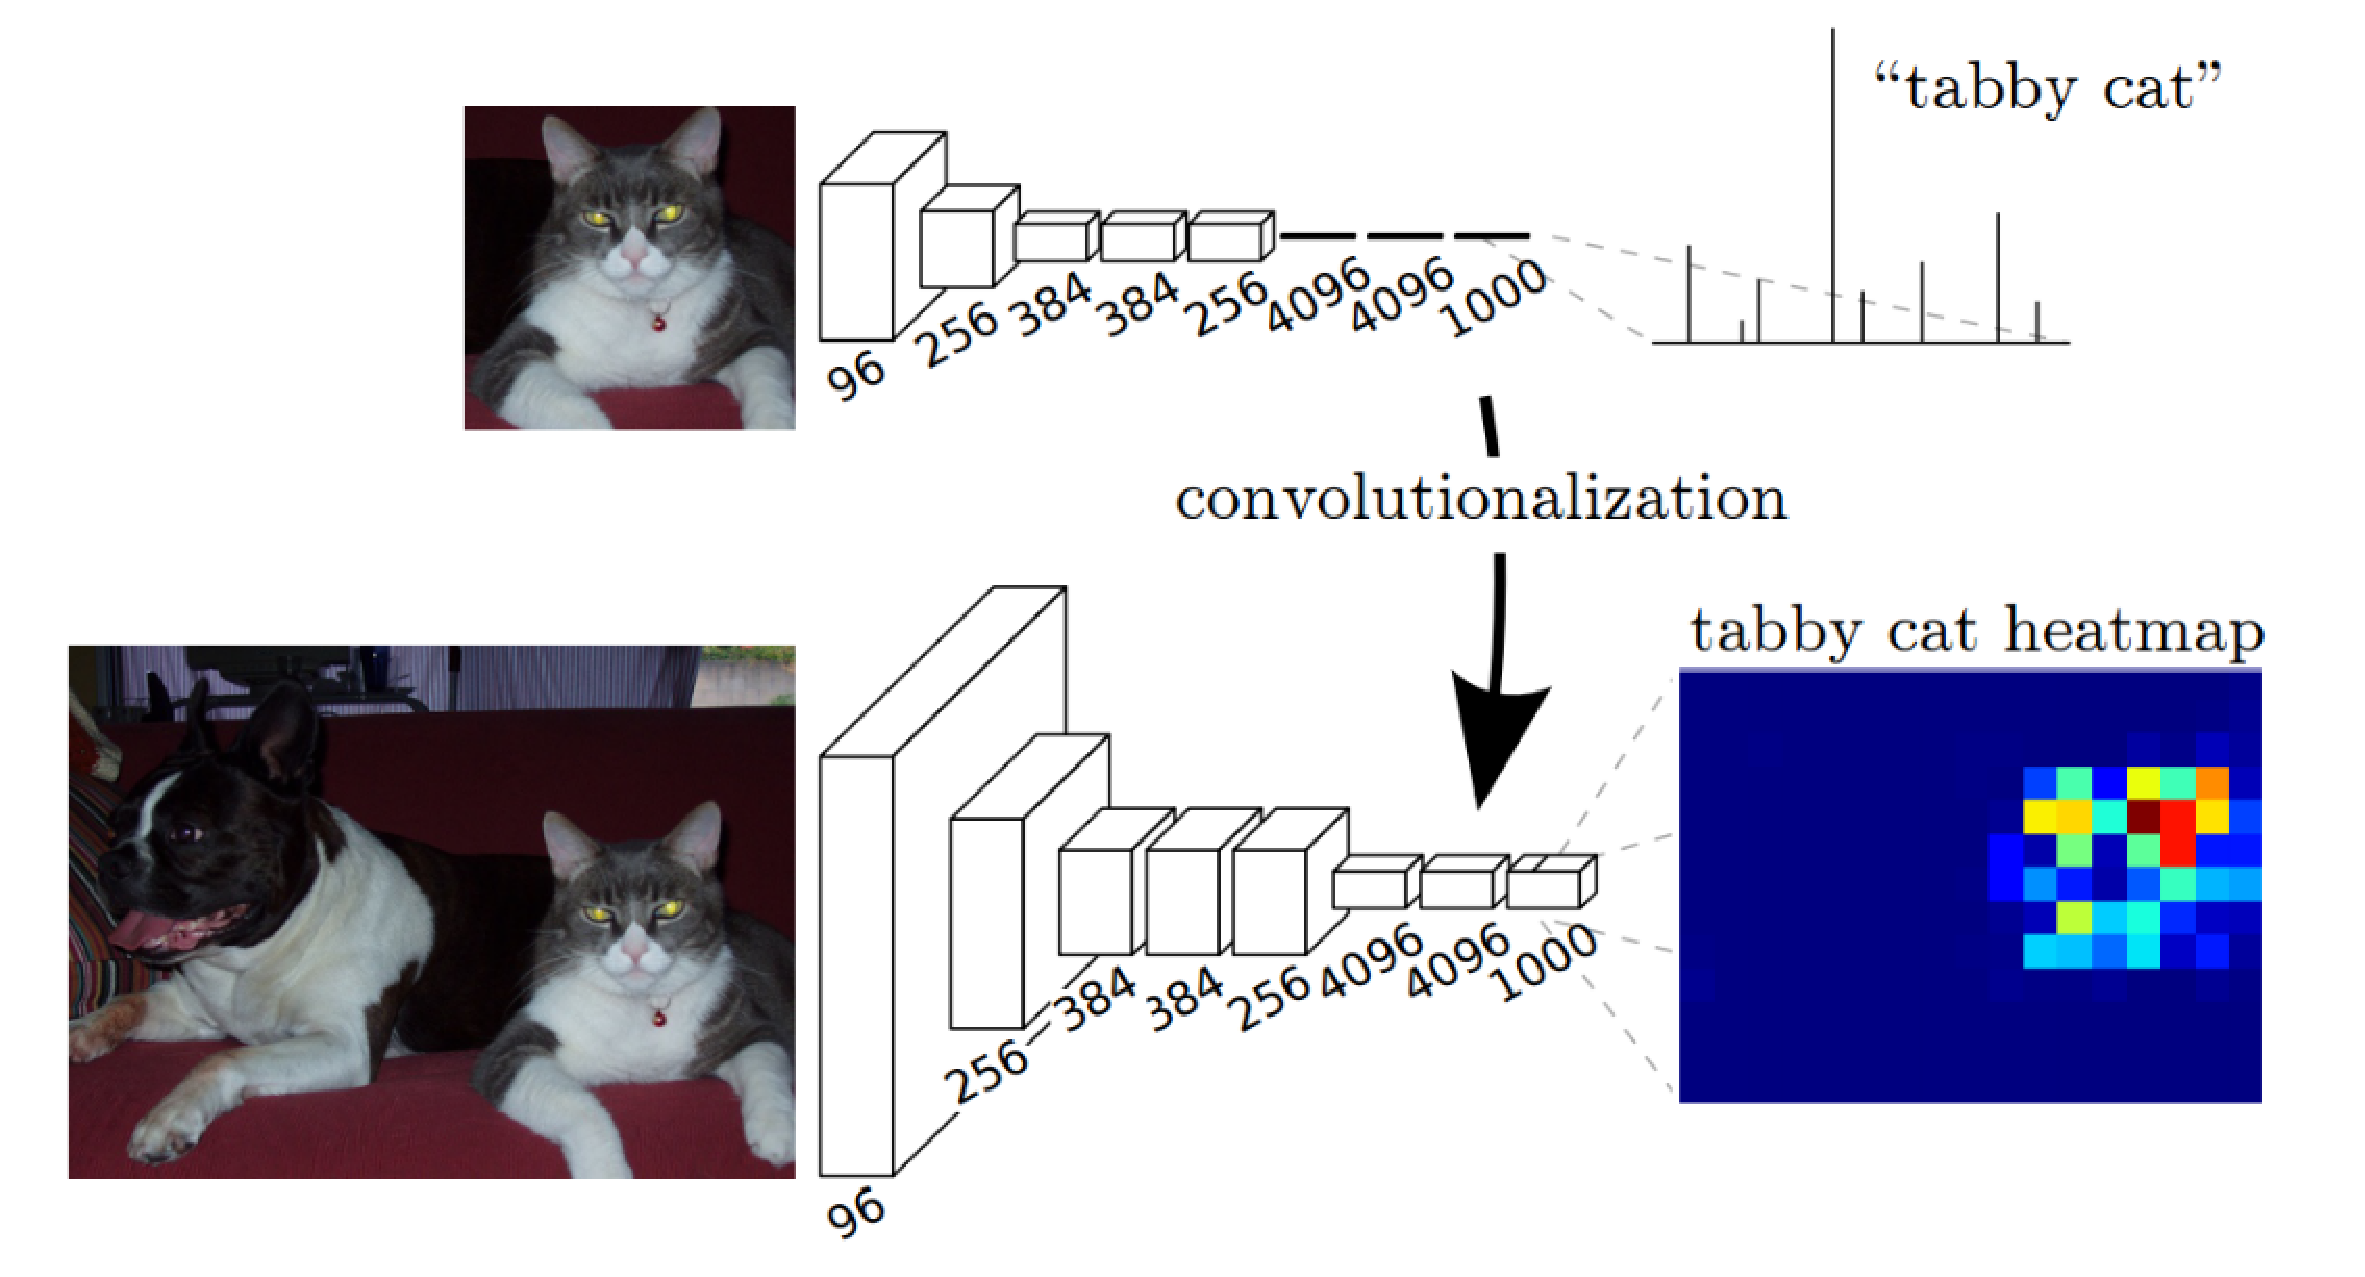
\includegraphics[width=\linewidth]{Figures/Segmentation/convolutionalization.eps}
	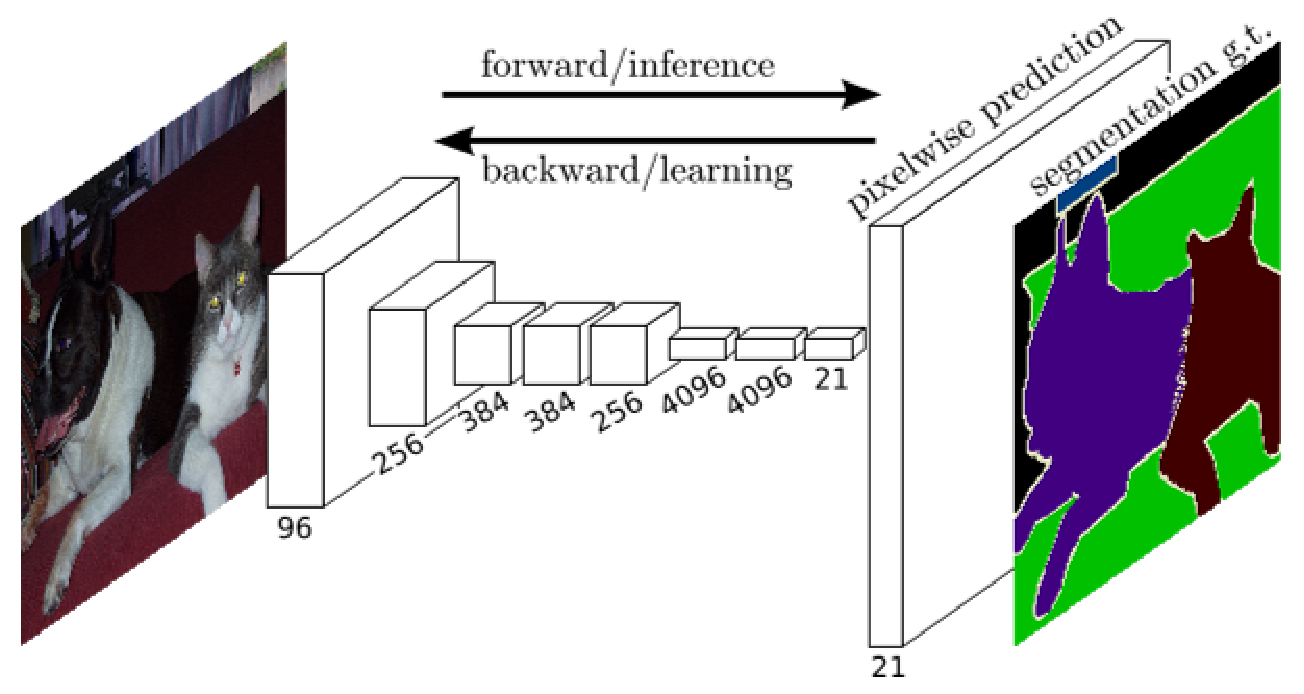
\includegraphics[width=0.86\linewidth]{Figures/Segmentation/fcn.eps}
	\caption{\acl{FCN} figure by Long \emph{et al.}\cite{Long2015}. Transforming a classification-purposed \ac{CNN} to produce spatial heatmaps by replacing fully connected layers with convolutional ones. Including a deconvolution layer for upsampling allows dense inference and learning for pixel labeling.}
	\label{fig:convolutionalization}
\end{figure}

Currently, the most successful state-of-the-art deep learning techniques for semantic segmentation stem from a common forerunner: the \emph{\acf{FCN}} by Long \emph{et al.}\cite{Long2015}. The insight of that approach was to take advantage of existing \acp{CNN} as powerful visual models that are able to learn hierarchies of features. They transformed those existing and well-known classification models -- AlexNet\cite{Krizhevsky2012}, \ac{VGG} (16-layer net)\cite{Simonyan2014}, GoogLeNet\cite{Szegedy2015}, and ResNet \cite{He2016} -- into fully convolutional ones by replacing the fully connected layers with convolutional ones to output spatial maps instead of classification scores. Those maps are upsampled using fractionally strided convolutions (also named deconvolutions \cite{Zeiler2011}\cite{Zeiler2014}) to produce dense per-pixel labeled outputs. This work is considered a milestone since it showed how \acp{CNN} can be trained end-to-end for this problem, efficiently learning how to make dense predictions for semantic segmentation with inputs of arbitrary sizes. This approach achieved a significant improvement in segmentation accuracy over traditional methods on standard datasets like PASCAL \ac{VOC}, while preserving efficiency at inference. For all those reasons, and other significant contributions, the \ac{FCN} is the cornerstone of deep learning applied to semantic segmentation. The convolutionalization process is shown in Figure \ref{fig:convolutionalization}.

Despite the power and flexibility of the \acs{FCN} model, it still lacks various features which hinder its application to certain problems and situations: its inherent spatial invariance does not take into account useful global context information, no instance-awareness is present by default, efficiency is still far from real-time execution at high resolutions, and it is not completely suited for unstructured data such as \acs{3D} point clouds or models. Those problems will be reviewed in this section, as well as the state-of-the-art solutions that have been proposed in the literature to overcome those hurdles. Table \ref{table:segmentation:methods} provides a summary of that review. It shows all reviewed methods (sorted by appearance order in the section), their base architecture, their main contribution, and a classification depending on the target of the work: accuracy, efficiency, training simplicity, sequence processing, multi-modal inputs, and \acs{3D} data. Each target is graded from one to three stars ($\star$) depending on how much focus puts the work on it, and a mark (\xmark) if that issue is not addressed. In addition, Figure \ref{fig:graph} shows a graph of the reviewed methods for the sake of visualization.

\begin{figure}[!b]
	\centering
	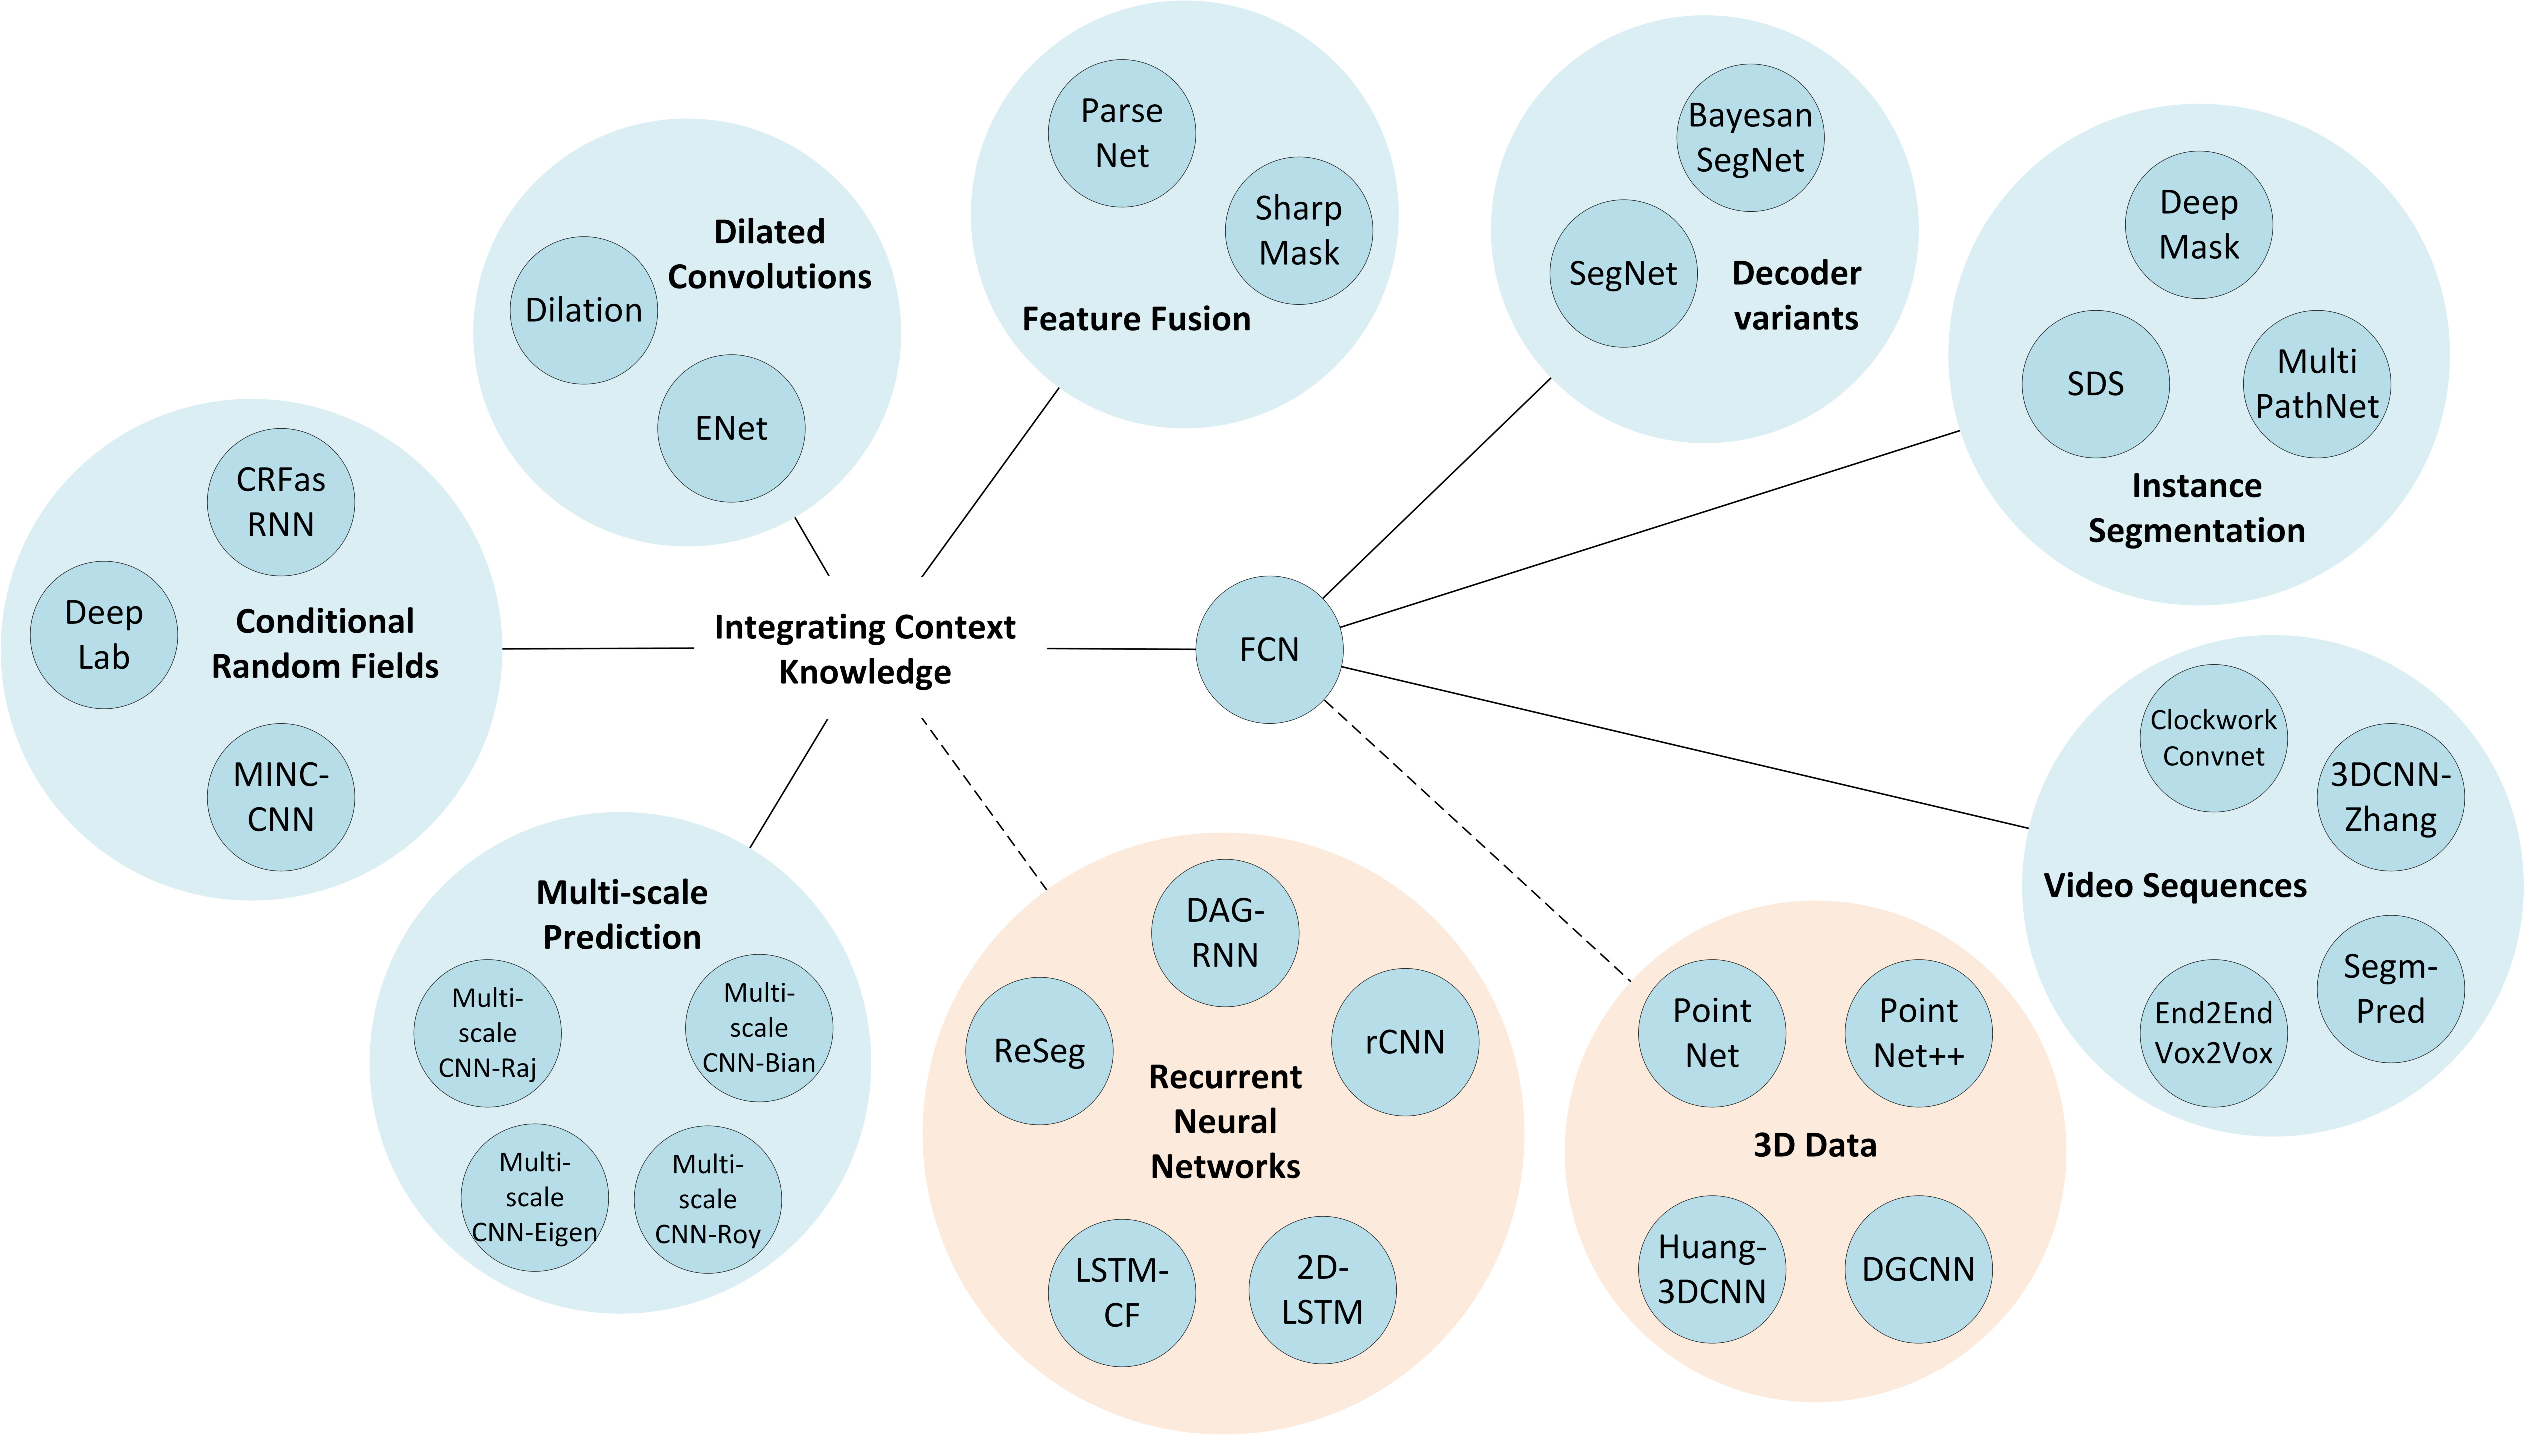
\includegraphics[width=\linewidth]{Figures/Segmentation/graph}
	\caption{Visualization of the reviewed methods. Considering the \ac{FCN} as the forerunner of all of them (at least from its basic idea), they all stem in various directions depending on their focus: most of them try to integrate context knowledge in one way or another while others tackle other problems such as instance segmentation, video sequences, and even \ac{3D} data.}
	\label{fig:graph}
\end{figure}

\subsection{Decoder Variants}

Apart from the \acs{FCN} architecture, other variants were developed to transform a network whose purpose was classification to make it suitable for segmentation. Arguably, \acs{FCN}-based architectures are more popular and successful, but other alternatives are also remarkable. In general terms, all of them take a network for classification, such as \acs{VGG}-16, and remove its fully connected layers. This part of the new segmentation network often receives the name of encoder and produce low-resolution image representations or feature maps. The problem lies on learning to decode or map those low-resolution images to pixel-wise predictions for segmentation. This part is named decoder and it is usually the divergence point in this kind of architectures.

SegNet\cite{Badrinarayanan2015} is a clear example of this divergence (see Figure \ref{fig:semseg:segnet}). The decoder stage of SegNet is composed by a set of upsampling and convolution layers which are at last followed by a softmax classifier to predict pixel-wise labels for an output which has the same resolution as the input image. Each upsampling layer in the decoder stage corresponds to a max-pooling one in the encoder part. Those layers upsample feature maps using the max-pooling indices from their corresponding feature maps in the encoder phase. The upsampled maps are then convolved with a set of trainable filter banks to produce dense feature maps. When the feature maps have been restored to the original resolution, they are fed to the softmax to produce the final segmentation.

\begin{figure}[!hbt]
	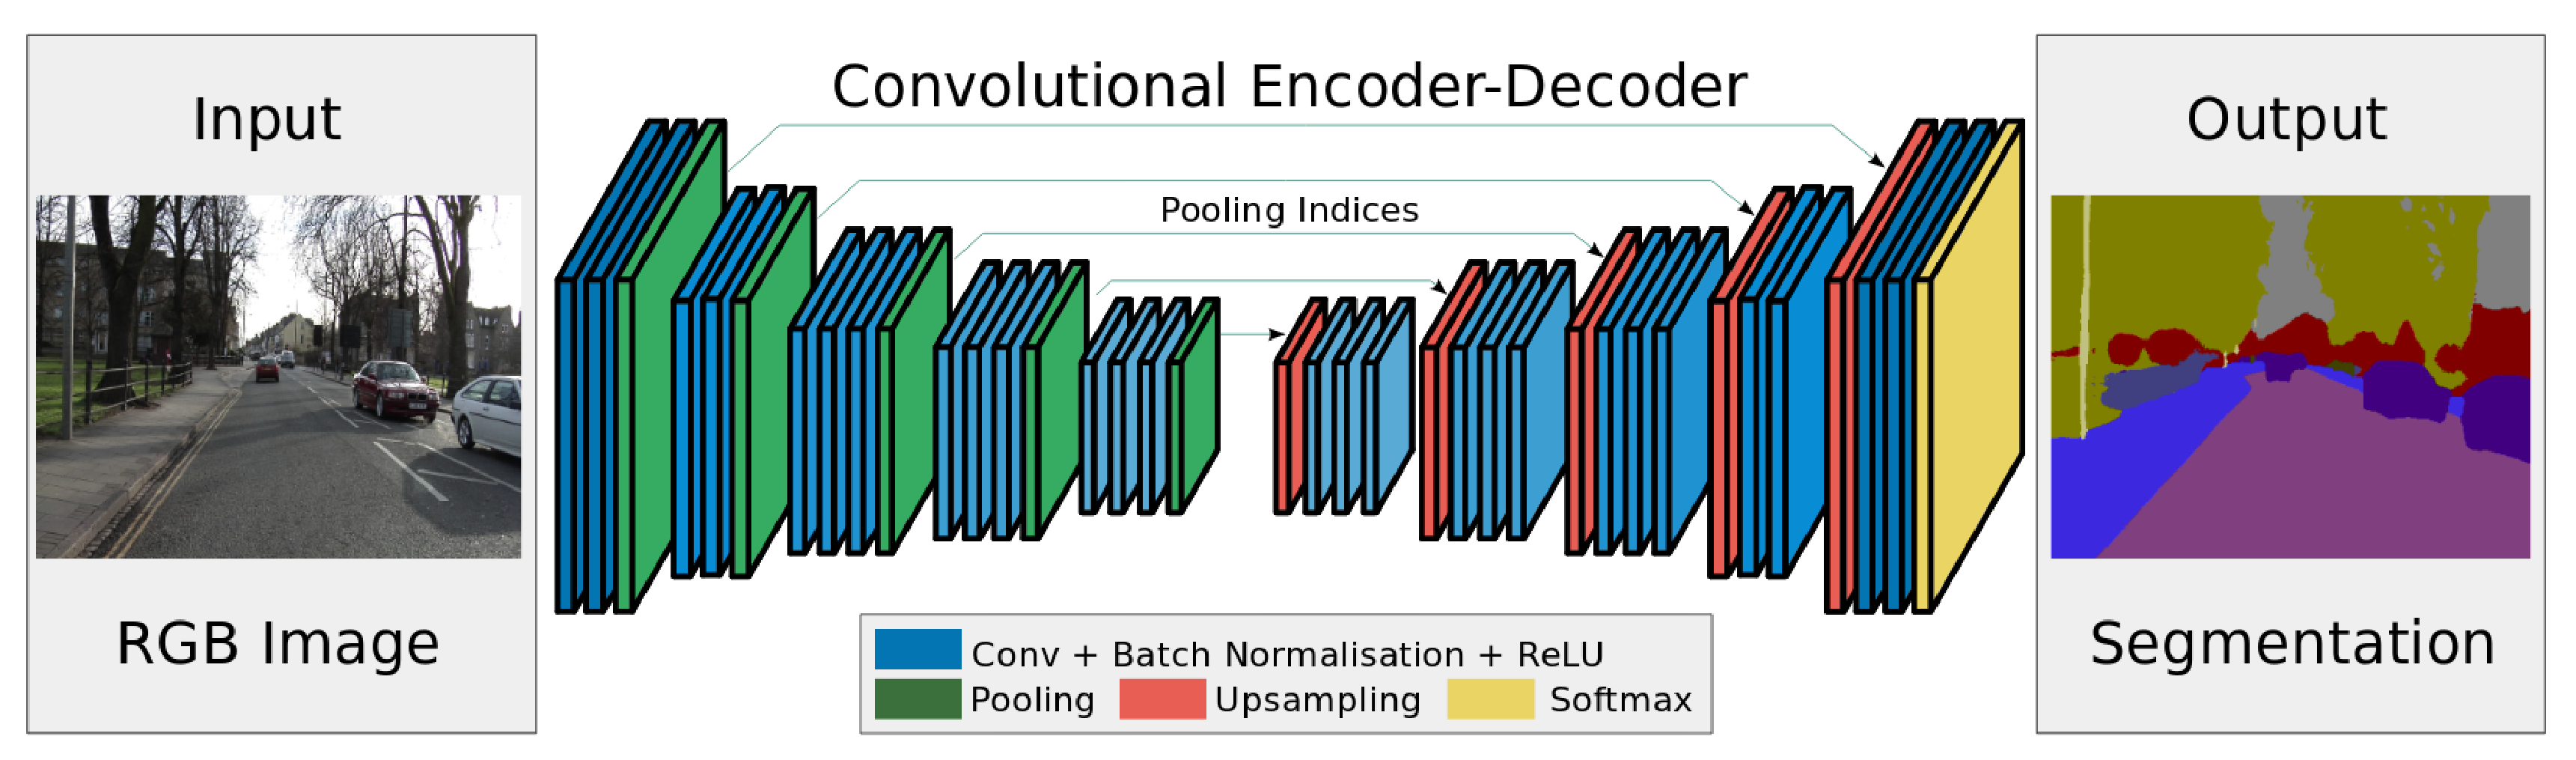
\includegraphics[width=\linewidth]{Figures/Segmentation/segnet.eps}
	\caption{SegNet architecture with an encoder and a decoder followed by a softmax classifier for pixel-wise classification. Figure extracted from \cite{Badrinarayanan2015}.}
	\label{fig:semseg:segnet}
\end{figure}

On the other hand, \acs{FCN}-based architectures make use of learnable deconvolution filters to upsample feature maps. After that, the upsampled feature maps are added element-wise to the corresponding feature map generated by the convolution layer in the encoder part. Figure \ref{fig:semseg:segnetvsfcn} shows a comparison of both approaches.

U-Net \cite{Ronneberger2015} is another example of a \acf{FCN} that has been used for image segmentation. It was initially proposed for biomedical image segmentation, but in the last years it has also been successfully used in other applications, such as aerial imagery \cite{Zhang2017} and regular foreground/background segmentation problems. It consists of a contracting path (downsampling) which captures context and a symmetric expanding path (upsampling) that enables precise localization. The architecture also has skip connections that allow the decoder at each stage to learn relevant features from the contracting path.

\begin{figure}[!hbt]
	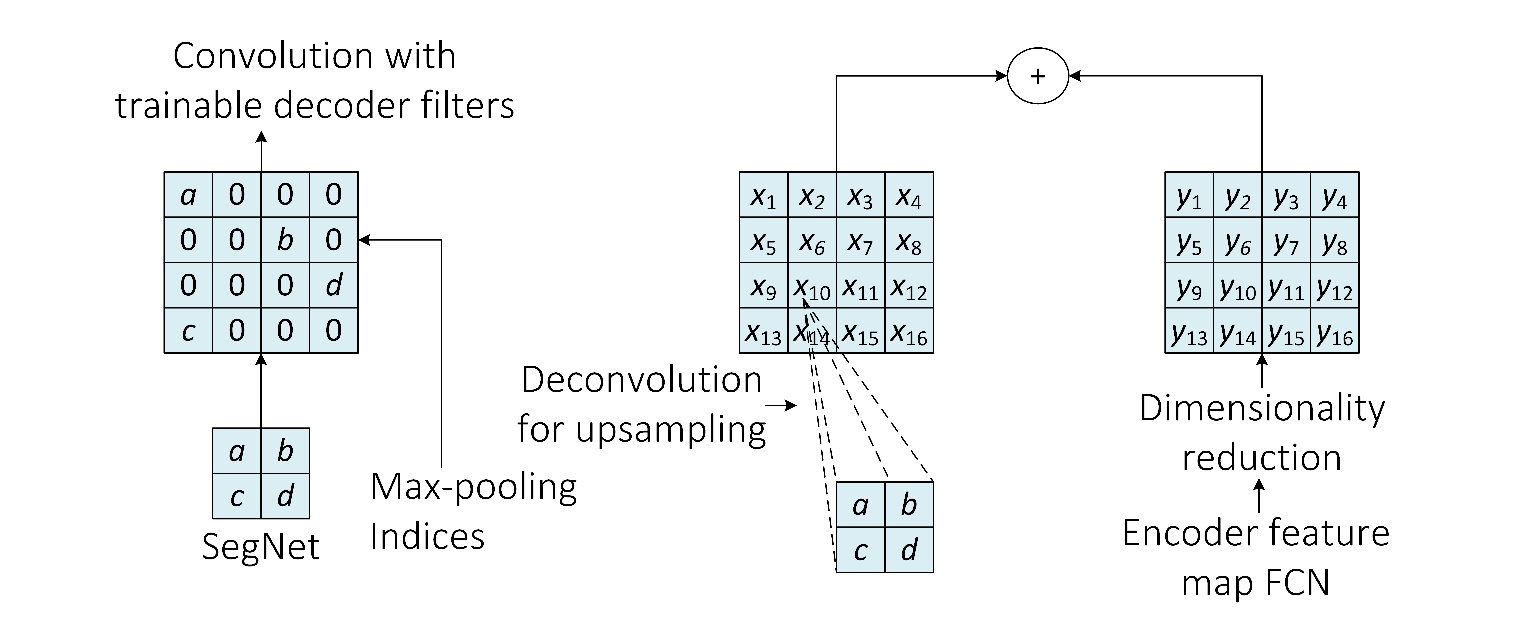
\includegraphics[width=\linewidth]{Figures/Segmentation/segnetvsfcn_rework.eps}
	\caption{Comparison of SegNet (left) and \acs{FCN} (right) decoders. While SegNet uses max-pooling indices from the corresponding encoder stage to upsample, \acs{FCN} learns deconvolution filters to upsample (adding the corresponding feature map from the encoder stage). Figure reproduced from \cite{Badrinarayanan2015}.}
	\label{fig:semseg:segnetvsfcn}
\end{figure}

\subsection{Integrating Context Knowledge}

Semantic segmentation is a problem that requires the integration of information from various spatial scales. It also implies balancing local and global information. On the one hand, fine-grained or local information is crucial to achieve good pixel-level accuracy. On the other hand, it is also important to integrate information from the global context of the image to be able to resolve local ambiguities.

Vanilla \acp{CNN} struggle with this balance. Pooling layers, which allow the networks to achieve some degree of spatial invariance and keep computational cost at bay, dispose of the global context information. Even purely \acp{CNN} -- without pooling layers -- are limited since the receptive field of their units can only grow linearly with the number of layers.

Many approaches can be taken to make \acp{CNN} aware of that global information: refinement as a post-processing step with \acp{CRF}, dilated convolutions, multi-scale aggregation, or even defer the context modeling to another kind of deep networks such as \acp{RNN}.

\subsubsection{\aclp{CRF}}

As we mentioned before, the inherent invariance to spatial transformations of \ac{CNN} architectures limits the very same spatial accuracy for segmentation tasks. One possible and common approach to refine the output of a segmentation system and boost its ability to capture fine-grained details is to apply a post-processing stage using a \acf{CRF}. \acp{CRF} enable the combination of low-level image information -- such as the interactions between pixels \cite{Rother2004}\cite{Shotton2009} -- with the output of multi-class inference systems that produce per-pixel class scores. That combination is especially important to capture long-range dependencies, which \acp{CNN} fail to consider, and fine local details.

The DeepLab models \cite{Chen2014a}\cite{Chen2016} make use of the fully connected pairwise \ac{CRF} by Krähenbühl and Koltun\cite{Koltun2011}\cite{Kraehenbuehl2013} as a separated post-processing step in their pipeline to refine the segmentation result. It models each pixel as a node in the field and employs one pairwise term for each pair of pixels no matter how far they lie (this model is known as dense or fully connected factor graph). By using this model, both short and long-range interactions are taken into account, rendering the system able to recover detailed structures in the segmentation that were lost due to the spatial invariance of the \ac{CNN}. Despite the fact that usually fully connected models are inefficient, this model can be efficiently approximated via probabilistic inference. Figure \ref{fig:semseg:crf-deeplab} shows the effect of this \ac{CRF}-based post-processing on the score and belief maps.

\begin{figure}[!hb]
	\hfill
	\begin{subfigure}{0.19\linewidth}
		\includegraphics[width=\linewidth]{Figures/Segmentation/scmapgt.eps}\\
		
\includegraphics[width=\linewidth]{Figures/Segmentation/beliefgt.eps}
		\caption{GT}
	\end{subfigure}
	\hfill
	\begin{subfigure}{0.19\linewidth}
		\includegraphics[width=\linewidth]{Figures/Segmentation/scmap001.eps}\\
		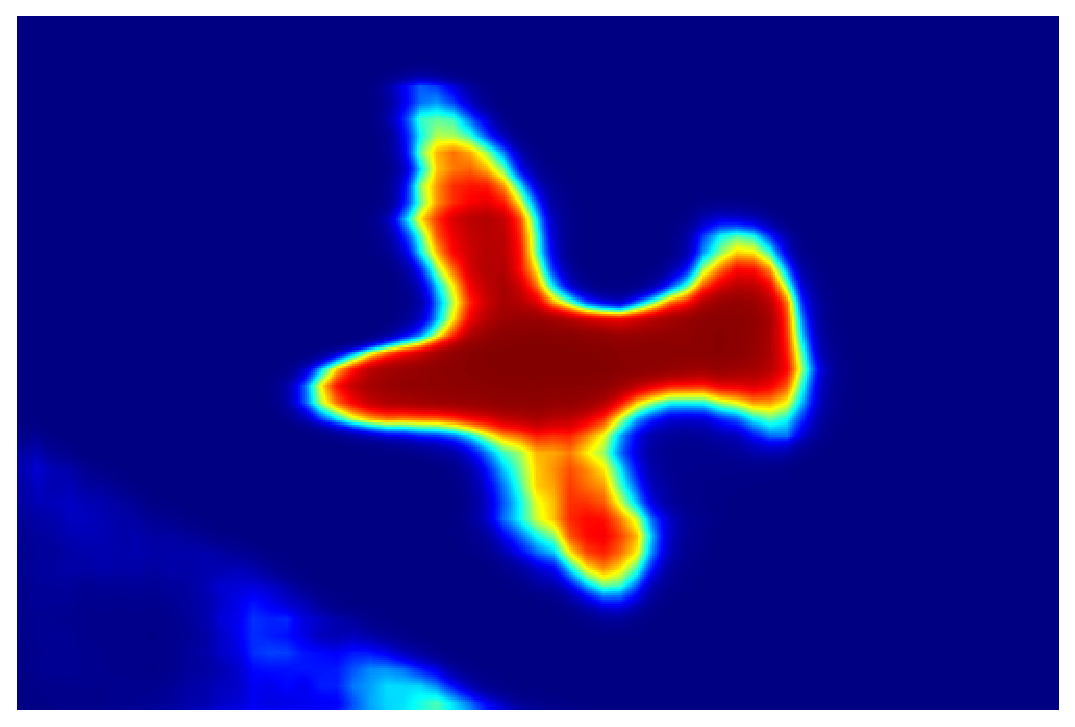
\includegraphics[width=\linewidth]{Figures/Segmentation/belief001.eps}
		\caption{\ac{CNN}out}
	\end{subfigure}
	\hfill
	\begin{subfigure}{0.19\linewidth}
		\includegraphics[width=\linewidth]{Figures/Segmentation/scmap002.eps}\\
		\includegraphics[width=\linewidth]{Figures/Segmentation/belief002.eps}
		\caption{\ac{CRF}it1}
	\end{subfigure}
	\hfill
	\begin{subfigure}{0.19\linewidth}
		\includegraphics[width=\linewidth]{Figures/Segmentation/scmap003.eps}\\
		\includegraphics[width=\linewidth]{Figures/Segmentation/belief003.eps}
		\caption{\ac{CRF}it2}
	\end{subfigure}
	\hfill
	\begin{subfigure}{0.19\linewidth}
		\includegraphics[width=\linewidth]{Figures/Segmentation/scmap004.eps}\\
		
\includegraphics[width=\linewidth]{Figures/Segmentation/belief004.eps}
		\caption{\ac{CRF}it10}
	\end{subfigure}
	\hfill
	\caption{\ac{CRF} refinement as shown by the authors of DeepLab\cite{Chen2014a}. The first row shows the score maps and the second one shows the belief maps.}
	\label{fig:semseg:crf-deeplab}
\end{figure}

The material recognition in the wild network by Bell \emph{et al.}\cite{Bell2015} makes use of various \acp{CNN} trained to identify patches in the \ac{MINC} database. Those \acp{CNN} are used on a sliding window fashion to classify those patches. Their weights are transferred to the same networks converted into \acp{FCN} by adding the corresponding upsampling layers. The outputs are averaged to generate a probability map. At last, the same \ac{CRF} from DeepLab, but discretely optimized, is applied to predict and refine the material at every pixel.

Another significant work applying a \ac{CRF} to refine the segmentation of a \ac{FCN} is the CRFasRNN by Zheng \emph{et al.}\cite{Zheng2015}. The main contribution of that work is the reformulation of the dense \ac{CRF} with pairwise potentials as an integral part of the network. By unrolling the mean-field inference steps as \acp{RNN}, they make it possible to fully integrate the \ac{CRF} with a \ac{FCN} and train the whole network end-to-end. This work demonstrates the reformulation of \acp{CRF} as \acp{RNN} to form a part of a deep network, in contrast with Pinheiro et al. \cite{Pinheiro2014} which employed \acp{RNN} to model large spatial dependencies.

\subsubsection{Dilated Convolutions}

Dilated convolutions, also named \emph{à-trous} convolutions, are a generalization of Kronecker-factored convolutional filters \cite{Zhou2015} which support exponentially expanding receptive fields without losing resolution. In other words, dilated convolutions are regular ones that make use of upsampled filters. The dilation rate $l$ controls that upsampling factor. As shown in Figure \ref{fig:semseg:dilated-convolution}, stacking $l$-dilated convolution makes the receptive fields grow exponentially while the number of parameters for the filters keeps a linear growth. This means that dilated convolutions allow efficient dense feature extraction on any arbitrary resolution. As a side note, it is important to remark that typical convolutions are just $1$-dilated convolutions.

\begin{figure}[!hbt]
	\hfill
	\begin{subfigure}{0.30\linewidth}
		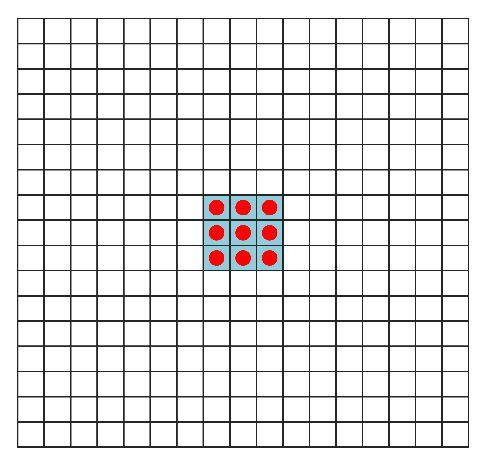
\includegraphics[width=\linewidth]{Figures/Segmentation/dilated_conv1_rework.eps}
		\caption{$1$-dilated}
		\label{fig:dilated-convolution:1}
	\end{subfigure}
	\hfill
	\begin{subfigure}{0.30\linewidth}
		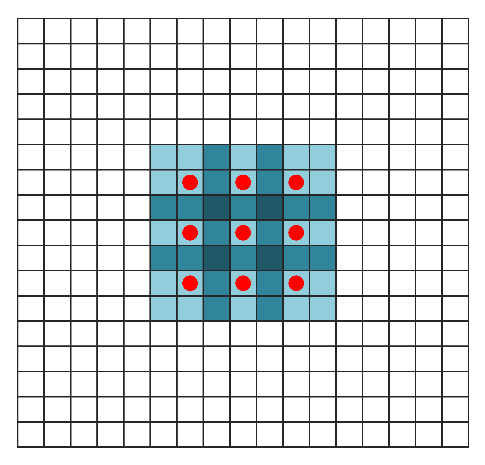
\includegraphics[width=\linewidth]{Figures/Segmentation/dilated_conv2_rework.eps}
		\caption{$2$-dilated}
		\label{fig:dilated-convolution:2}
	\end{subfigure}
	\hfill
	\begin{subfigure}{0.30\linewidth}
		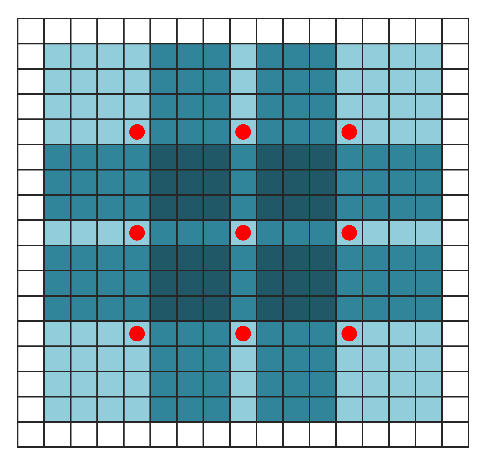
\includegraphics[width=\linewidth]{Figures/Segmentation/dilated_conv3_rework.eps}
		\caption{$3$-dilated}
		\label{fig:dilated-convolution:3}
	\end{subfigure}
	\hfill
	\caption{As shown in \cite{Yu2015}, dilated convolution filters with various dilation rates: (\protect\subref{fig:dilated-convolution:1}) $1$-dilated convolutions in which each unit has a $3\times3$ receptive fields, (\protect\subref{fig:dilated-convolution:2}) $2$-dilated ones with $7\times7$ receptive fields, and (\protect\subref{fig:dilated-convolution:3}) $3$-dilated convolutions with $15\times15$ receptive fields.}
	\label{fig:semseg:dilated-convolution}
\end{figure}

In practice, it is equivalent to dilating the filter before doing the usual convolution. That means expanding its size, according to the dilation rate, while filling the empty elements with zeros. In other words, the filter weights are matched to distant elements which are not adjacent if the dilation rate is greater than one. Figure \ref{fig:semseg:dilated-convolution-filter} shows examples of dilated filters.

\begin{figure}[!hbt]
	\centering
	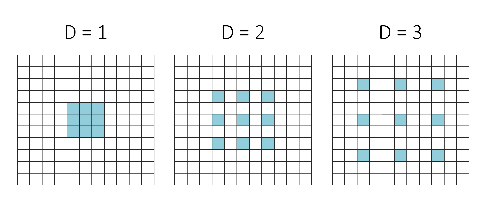
\includegraphics[width=\linewidth]{Figures/Segmentation/dilatedconvolutions_rework.eps}
	\caption{Filter elements (green) matched to input elements when using $3\times3$ dilated convolutions with various dilation rates. From left to right: $1, 2, $ and $3$.}
	\label{fig:semseg:dilated-convolution-filter}
\end{figure}

The most important works that make use of dilated convolutions are the multi-scale context aggregation module by Yu \emph{et al.}\cite{Yu2015}, the already mentioned DeepLab (its improved version)\cite{Chen2016}, and the real-time network ENet\cite{Paszke2016}. All of them use combinations of dilated convolutions with increasing dilation rates to have wider receptive fields with no additional cost and without overly downsampling the feature maps. Those works also show a common trend: dilated convolutions are tightly coupled to multi-scale context aggregation as we will explain in the following section.

\subsubsection{Multi-scale Prediction}

Another possible way to deal with context knowledge integration is the use of multi-scale predictions. Almost every single parameter of a \acs{CNN} affects the scale of the generated feature maps. In other words, the very same architecture will have an impact on the number of pixels of the input image which correspond to a pixel of the feature map. This means that the filters will implicitly learn to detect features at specific scales (presumably with certain invariance degree). Furthermore, those parameters are usually tightly coupled to the problem at hand, making it difficult for the models to generalize to different scales. One possible way to overcome that obstacle is to use multi-scale networks which generally make use of multiple networks that target different scales and then merge the predictions to produce a single output.

\begin{figure}[!htb]
	\centering
	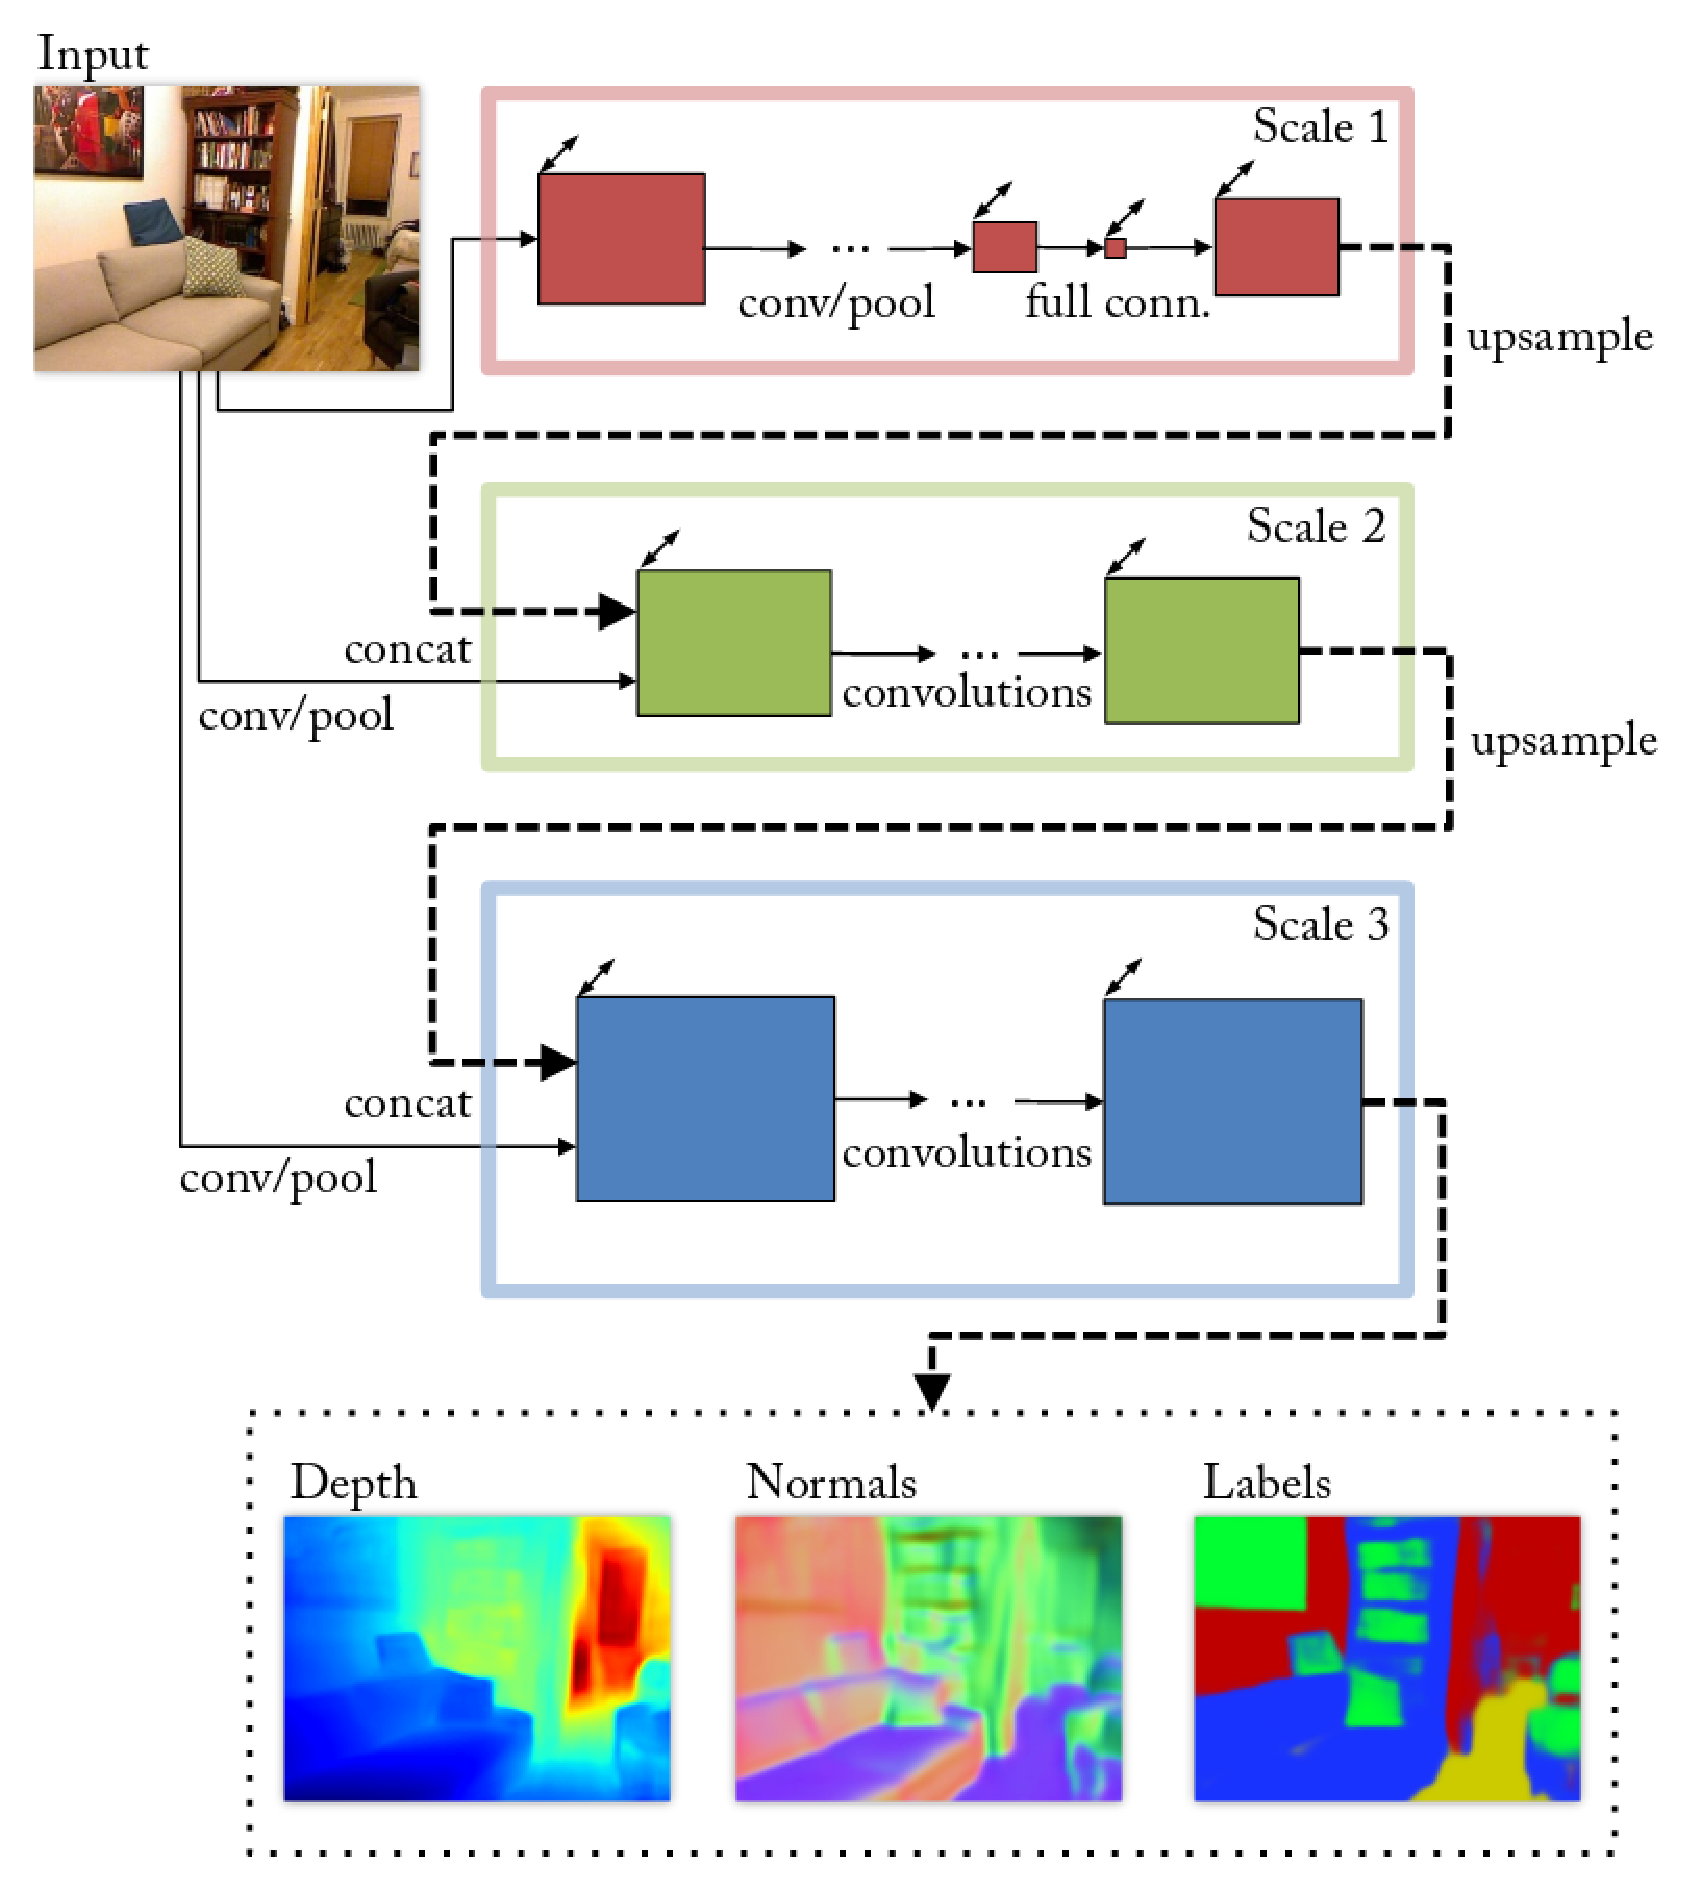
\includegraphics[width=0.86\linewidth]{Figures/Segmentation/eigenmultiscale.eps}
	\caption{Multi-scale \acs{CNN} architecture proposed by Eigen \emph{et al.}\cite{Eigen2015}. The network progressively refines the output using a sequence of scales to estimate depth, normals, and also perform semantic segmentation over an \acs{RGB} input. Figure extracted from \cite{Eigen2015}.}
	\label{fig:semseg:eigen-multiscale}
\end{figure}

Raj \emph{et al.}\cite{Raj2015} propose a multi-scale version of a fully convolutional \acs{VGG}-16. That network has two paths, one that processes the input at the original resolution and another one which doubles it. The first path goes through a shallow convolutional network. The second one goes through the fully convolutional \acs{VGG}-16 and an extra convolutional layer. The result of that second path is upsampled and combined with the result of the first path. That concatenated output then goes through another set of convolutional layers to generate the final output. As a result, the network becomes more robust to scale variations.

Roy \emph{et al.}\cite{Roy2016} take a different approach using a network composed by four multi-scale \acp{CNN}. Those four networks have the same architecture introduced by Eigen \emph{et al.} \cite{Eigen2015}. One of those networks is devoted to finding semantic labels for the scene. That network extracts features from a progressively coarse-to-fine sequence of scales (see Figure \ref{fig:semseg:eigen-multiscale}).

Another remarkable work is the network proposed by Bian \emph{et al.}\cite{Bian2016}. That network is a composition of $n$ \acp{FCN} which operate at different scales. The features extracted from the networks are fused together (after the necessary upsampling with an appropriate padding) and then they go through an additional convolutional layer to produce the final segmentation. The main contribution of this architecture is the two-stage learning process which involves, first, training each network independently, then the networks are combined and the last layer is fine-tuned. This multi-scale model allows to add an arbitrary number of newly trained networks in an efficient manner.

\subsubsection{Feature Fusion}

Another way of adding context information to a fully convolutional architecture for segmentation is feature fusion. This technique consists of merging a global feature (extracted from a previous layer in a network) with a more local feature map extracted from a subsequent layer. Common architectures such as the original \acs{FCN} make use of skip connections to perform a late fusion by combining the feature maps extracted from different layers (see Figure \ref{fig:semseg:skipconnections}).

\begin{figure}[!hbt]
	\centering
	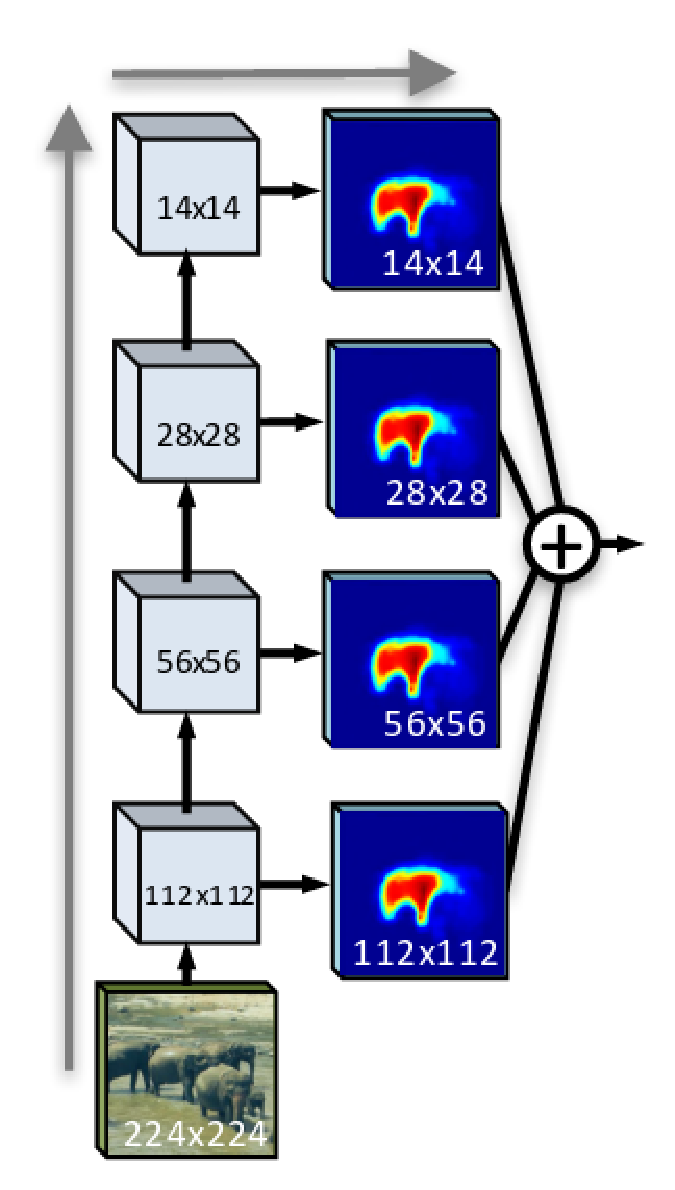
\includegraphics[width=0.45\linewidth]{Figures/Segmentation/sharpmaskskip.eps}
	\caption{Skip-connection-like architecture, which performs late fusion of feature maps as if making independent predictions for each layer and merging the results. Figure extracted from \cite{Pinheiro2016}.}
	\label{fig:semseg:skipconnections}
\end{figure}

Another approach is performing early fusion. This approach is taken by ParseNet\cite{Liu2015} in their context module. The global feature is unpooled to the same spatial size as the local feature and then they are concatenated to generate a combined feature that is used in the next layer or to learn a classifier. Figure \ref{fig:parsenet-module} shows a representation of that process.

\begin{figure}[!hbt]
	\centering
	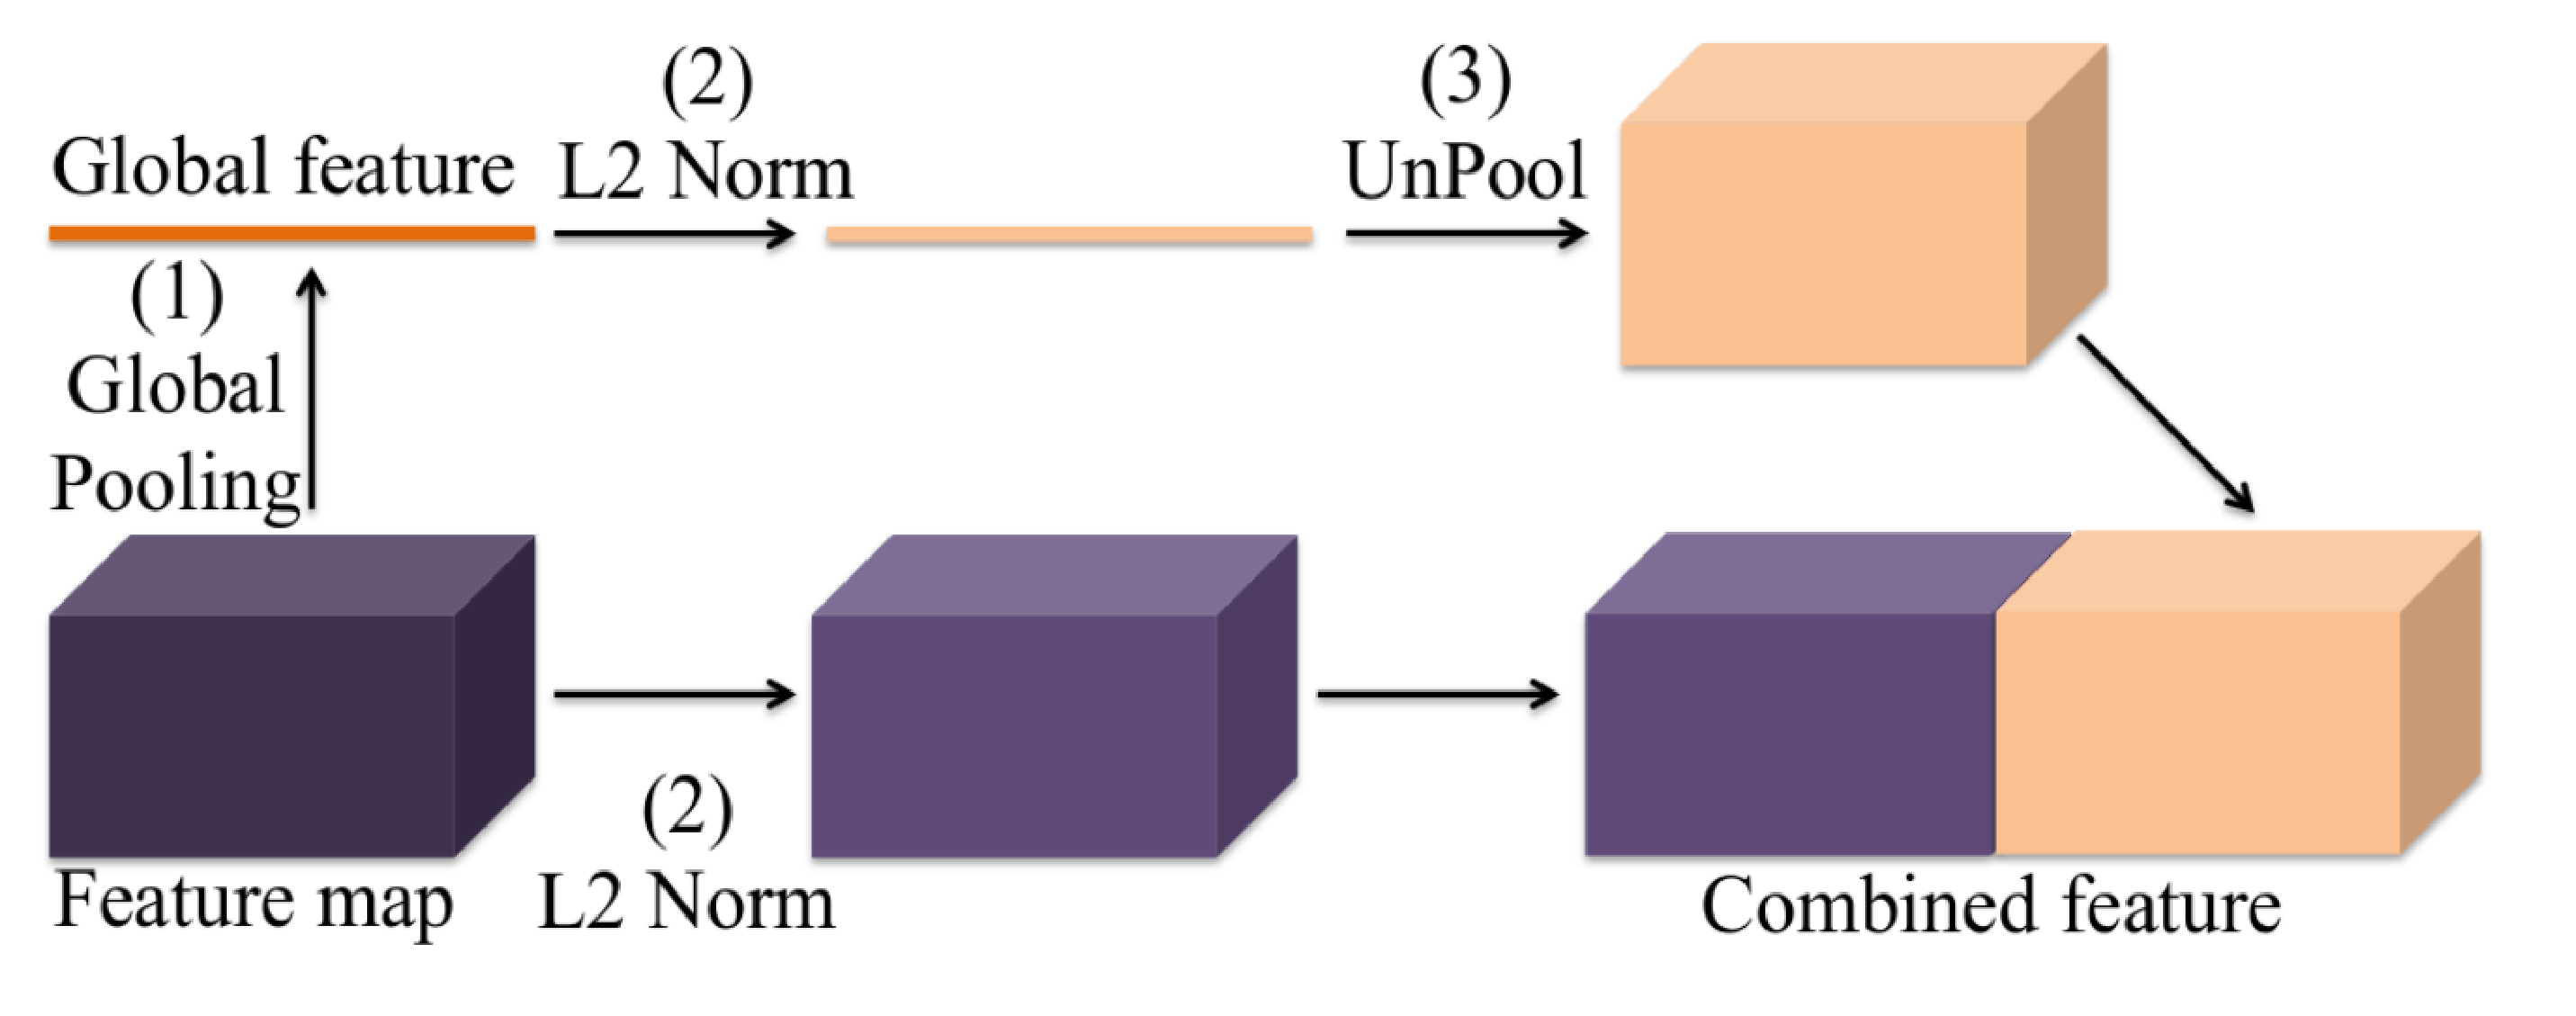
\includegraphics[width=\linewidth]{Figures/Segmentation/parsenetmodule.eps}
	\caption{ParseNet context module overview in which a global feature (from a previous layer) is combined with the feature of the next layer to add context information. Figure extracted from \cite{Liu2015}.}
	\label{fig:parsenet-module}
\end{figure}

This feature fusion idea was continued by Pinheiro \emph{et al.} in their SharpMask network \cite{Pinheiro2016}, which introduced a progressive refinement module to incorporate features from the previous layer to the next in a top-down architecture. This work will be reviewed later since it is mainly focused on instance segmentation.

In contrast to the pooling operation performed by ParseNet to incorporate global features and in addition to dilated \acsp{FCN} \cite{Chen2014a}\cite{Yu2015}, pyramid pooling empirically demonstrates the capability of global feature extraction by different-region-based context aggregation \cite{Zhao2016}. Figure \ref{fig:semseg:pspnet} shows \acfp{PSPNet} \footnote{\url{https://github.com/hszhao/PSPNet}} which provide a pyramid parsing module focused into feature fusion at four different pyramid scales in order to embed global contexts from complex scenes. Pyramid levels and size of each level can be arbitrarily modified. The better performance of \acs{PSPNet} facing \acsp{FCN}-based models lies to: (1) the lack of ability in collecting contextual information, (2) the absence of category relationships and (3) not using sub-regions. This approach achieves state-of-the-art performance on various datasets. 

\begin{figure*}[!hbt]
	\centering
	\includegraphics[width=\textwidth]{Figures/Segmentation/pspnet.eps}
	\caption{\acs{PSPNet} architecture. Initial feature maps (b) are extracted from input images (a) by using a pretrained ResNet \cite{He2016} alongside dilated network strategy. Pyramid pooling module (c) covers from the whole, half of to small regions of the image. Finally, initial feature map is concatenated with pooling module output and applying a convolution layer final predicted maps (d) are generated. Figure extracted from \cite{Zhao2016}.}
	\label{fig:semseg:pspnet}
\end{figure*}

\subsubsection{\aclp{RNN}}

\begin{figure*}[!t]
	\centering
	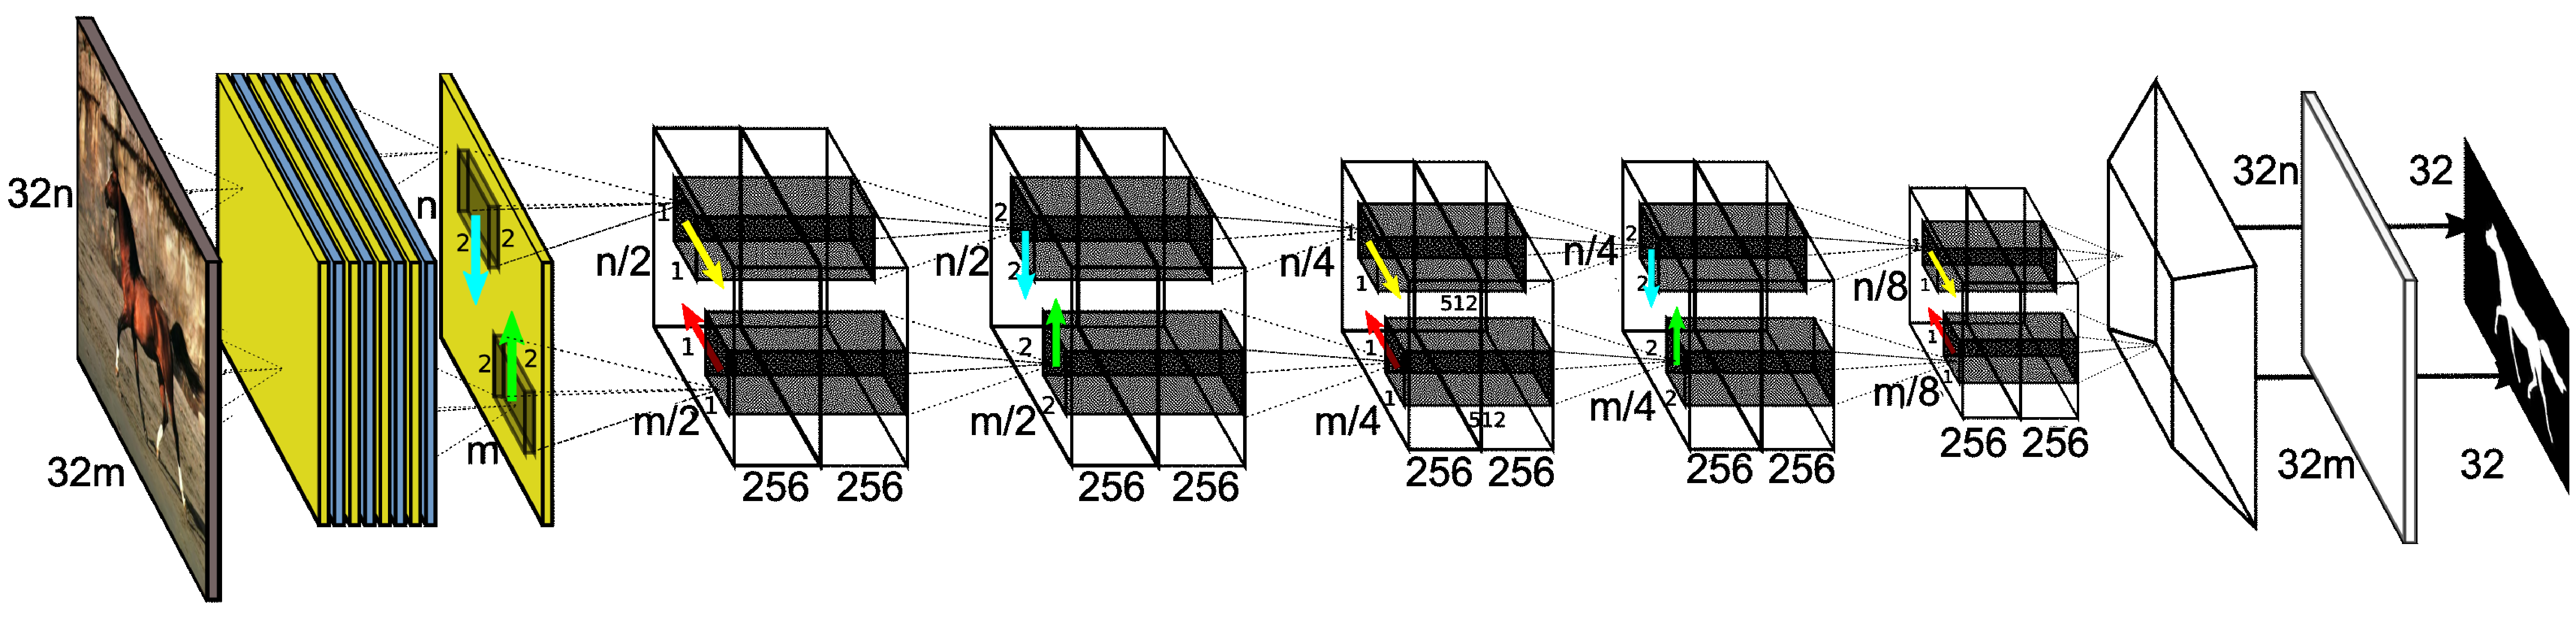
\includegraphics[width=\linewidth]{Figures/Segmentation/reseg_base.eps}
	\caption{Representation of ReSeg network. VGG-16 convolutional layers are represented by the blue and yellow first layers. The rest of the architecture is based on the ReNet approach with fine-tuning purposes. Figure extracted from \cite{Visin2016}.}
	\label{fig:semseg:reseg-network}
\end{figure*}

As we noticed, \acp{CNN} have been successfully applied to multi-dimensional data, such as images. Nevertheless, these networks rely on hand specified kernels limiting the architecture to local contexts. Taking advantage of its topological structure, \aclp{RNN} have been successfully applied for modeling short- and long-temporal sequences. In this way and by linking together pixel-level and local information, \acp{RNN} are able to successfully model global contexts and improve semantic segmentation. However, one important issue is the lack of a natural sequential structure in images and the focus of standard vanilla \acp{RNN} architectures on one-dimensional inputs.  
	
Based on ReNet model for image classification Visin \emph{et al.}\cite{Visin2015} proposed an architecture for semantic segmentation called ReSeg \cite{Visin2016} represented in Figure \ref{fig:semseg:reseg-network}. In this approach, the input image is processed with the first layers of the \acs{VGG}-16 network \cite{Simonyan2014}, feeding the resulting feature maps into one or more ReNet layers for fine-tuning. Finally, feature maps are resized using upsampling layers based on transposed convolutions. In this approach \acp{GRU} have been used as they strike a good performance balance regarding memory usage and computational power. Vanilla \acsp{RNN} have problems modeling long-term dependencies mainly due to the vanishing gradients problem. Several derived models such as \ac{LSTM} networks \cite{Hochreiter1997} and \acp{GRU} \cite{Cho2014} are the state-of-art in this field to avoid such problem. 

Inspired on the same ReNet architecture, a novel \ac{LSTM-CF} model for scene labeling was proposed by \cite{ZhenLi2016}. In this approach, they use two different data sources: \acs{RGB} and depth. The \acs{RGB} pipeline relies on a variant of the DeepLab architecture \cite{Chen2014} concatenating features at three different scales to enrich feature representation (inspired by \cite{Li2016}). The global context is modeled vertically over both, depth and photometric data sources, concluding with a horizontal fusion in both direction over these vertical contexts.

As we noticed, modeling image global contexts is related to 2D recurrent approaches by unfolding vertically and horizontally the network over the input images. Based on the same idea, Byeon et al. \cite{Byeon2015} purposed a simple 2D \ac{LSTM}-based architecture in which the input image is divided into non-overlapping windows which are fed into four separate \acp{LSTM} memory blocks. This work emphasizes its low computational complexity on a single-core CPU and the model simplicity. 

Another approach for capturing global information relies on using bigger input windows in order to model larger contexts. Nevertheless, this reduces images resolution and also implies several problems regarding to window overlapping. However, Pinheiro et al. \cite{Pinheiro2014} introduced \acp{rCNN} which recurrently train with different input window sizes taking into account previous predictions by using a different input window sizes. In this way, predicted labels are automatically smoothed increasing the performance.

Undirected cyclic graphs (UCGs) were also adopted to model image contexts for semantic segmentation \cite{Shuai2015}. Nevertheless, \acp{RNN} are not directly applicable to UCG and the solution is decomposing it into several directed graphs (DAGs). In this approach, images are processed by three different layers: image feature map produced by \acs{CNN}, model image contextual dependencies with DAG-RNNs, and deconvolution layer for upsampling feature maps. This work demonstrates how \acp{RNN} can be used together with graphs to successfully model long-range contextual dependencies, overcoming state-of-the-art approaches in terms of performance.

\subsection{Instance Segmentation}

Instance segmentation is considered the next step after semantic segmentation and at the same time the most challenging problem in comparison with the rest of low-level pixel segmentation techniques. Its main purpose is to represent objects of the same class splitted into different instances. The automation of this process is not straightforward, thus the number of instances is initially unknown and the evaluation of performed predictions is not pixel-wise such as in semantic segmentation. Consequently, this problem remains partially unsolved but the interest in this field is motivated by its potential applicability. Instance labeling provides us extra information for reasoning about occlusion situations, also counting the number of elements belonging to the same class and for detecting a particular object for grasping in robotics tasks, among many other applications.

For this purpose, Hariharan et al. \cite{Hariharan2014} proposed a \ac{SDS} method in order to improve performance over already existing works. Their pipeline uses, firstly, a bottom-up hierarchical image segmentation and object candidate generation process called \ac{MCG} \cite{Arbelaez2014} to obtain region proposals. For each region, features are extracted by using an adapted version of the \ac{R-CNN} \cite{Girshick2014}, which is fine-tuned using bounding boxes provided by the \ac{MCG} method instead of selective search and also alongside region foreground features. Then, each region proposal is classified by using a linear \ac{SVM} on top of the \acs{CNN} features. Finally, and for refinement purposes, \ac{NMS} is applied to the previous proposals.

Later, Pinheiro et al. \cite{Pinheiro2015} presented DeepMask model, an object proposal approach based on a single ConvNet. This model predicts a segmentation mask for an input patch and the likelihood of this patch for containing an object. The two tasks are learned jointly and computed by a single network, sharing most of the layers except last ones which are task-specific. 

\begin{figure}[!hbt]
	\centering
	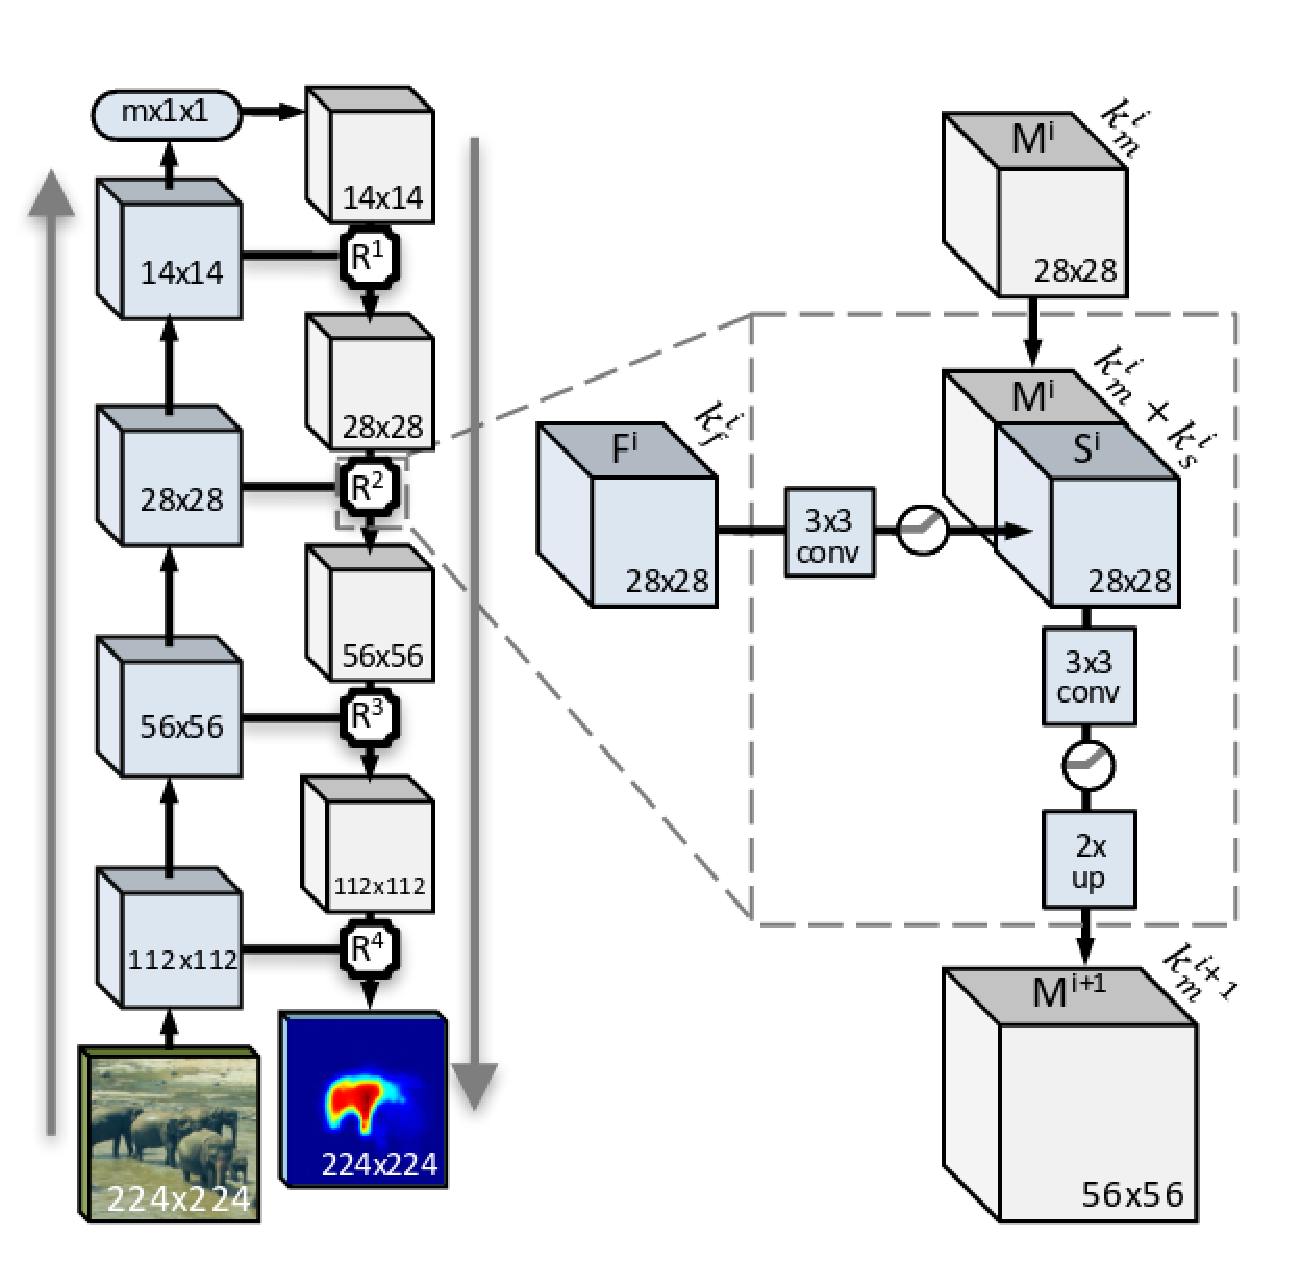
\includegraphics[width=0.75\linewidth]{Figures/Segmentation/sharpmaskmodule.eps}
	\caption{SharpMask's top-down architecture with progressive refinement using their signature modules. That refinement merges spatially rich information from lower-level features with high-level semantic cues encoded in upper layers. Figure extracted from \cite{Pinheiro2015}.}
	\label{fig:semseg:sharpmask-refinement-module}
\end{figure}

Based on the DeepMask architecture as a starting point due to its effectiveness, the same authors presented a novel architecture for object instance segmentation implementing a top-down refinement process \cite{Pinheiro2016} and achieving a better performance in terms of accuracy and speed. The goal of this process is to efficiently merge low-level features with high-level semantic information from upper network layers. The process consisted in different refinement modules stacked together (one module per pooling layer), with the purpose of inverting pooling effect by generating a new upsampled object encoding. Figure \ref{fig:semseg:sharpmask-refinement-module} shows the refinement module in SharpMask.

Another approach, based on Fast R-CNN as a starting point and using DeepMask object proposals instead of Selective Search was presented by Zagoruyko et al \cite{Zagoruyko2016}. This combined system called MultiPath classifier, improved performance over COCO dataset and supposed three modifications to Fast R-CNN: improving localization with an integral loss, provide context by using foveal regions and finally skip connections to give multi-scale features to the network. The system achieved a 66\% improvement over the baseline Fast R-CNN.

As we have seen, most of the methods mentioned above rely on existing object detectors limiting in this way model performance. Even so, instance segmentation process remains an unresolved research problem and the mentioned works are only a small part of this challenging research topic. 

\subsection{\acs{RGB-D} Data}

As we noticed, a significant amount of work has been done in semantic segmentation by using photometric data. Nevertheless, the use of structural information was spurred on with the advent of low-cost \acs{RGB-D} sensors which provide useful geometric cues extracted from depth information. Several works focused on \acs{RGB-D} scene segmentation have reported an improvement in the fine-grained labeling precision by using depth information and not only photometric data. Using depth information for segmentation is considered more challenging because of the unpredictable variation of scene illumination alongside incomplete representation of objects due to complex occlusions. However, various works have successfully made use of depth information to increase accuracy.

The use of depth images with approaches focused on photometric data is not straightforward. Depth data needs to be encoded with three channels at each pixel as if it was an \acs{RGB} images. Different techniques such as \ac{HHA} \cite{Gupta2014} are used for encoding the depth into three channels as follows: horizontal disparity, height above ground, and the angle between local surface normal and the inferred gravity direction. In this way, we can input depth images to models designed for \acs{RGB} data and improve in this way the performance by learning new features from structural information. Several works such as \cite{ZhenLi2016} are based on this encoding technique.

In the literature, related to methods that use \acs{RGB-D} data, we can also find some works that leverage a multi-view approach to improve existing single-view works.

Zeng \emph{et al.}\cite{Zeng2016} present an object segmentation approach that leverages multi-view \acs{RGB-D} data and deep learning techniques. RGB-D images captured from each viewpoint are fed to a \acs{FCN} network which returns a 40-class probability for each pixel in each image. Segmentation labels are threshold by using three times the standard deviation above the mean probability across all views. Moreover, in this work, multiple networks for feature extraction were trained (AlexNet \cite{Krizhevsky2012} and \acs{VGG}-16 \cite{Simonyan2014}), evaluating the benefits of using depth information. They found that adding depth did not yield any major improvements in segmentation performance, which could be caused by noise in the depth information. The described approach was presented during the 2016 Amazon Picking Challenge. This work is a minor contribution towards multi-view deep learning systems since \acs{RGB} images are independently fed to a \acs{FCN} network.

Ma \emph{et al.}\cite{Ma2017} propose a novel approach for object-class segmentation using a multi-view deep learning technique. Multiple views are obtained from a moving RGB-D camera. During the training stage, camera trajectory is obtained using an RGB-D SLAM technique, then RGB-D images are warped into ground-truth annotated frames in order to enforce multi-view consistency for training. The proposed approach is based on FuseNet\cite{Hazirbas2016}, which combines \acs{RGB} and depth images for semantic segmentation, and improves the original work by adding multi-scale loss minimization.

\subsection{\acs{3D} Data}

\acs{3D} geometric data such as point clouds or polygonal meshes are useful representations thanks to their additional dimension which provides methods with rich spatial information that is intuitively useful for segmentation. However, the vast majority of successful deep learning segmentation architectures -- \acp{CNN} in particular -- are not originally engineered to deal with unstructured or irregular inputs such as the aforementioned ones. In order to enable weight sharing and other optimizations in convolutional architectures, most researchers have resorted to 3D voxel grids or projections to transform unstructured and unordered point clouds or meshes into regular representations before feeding them to the networks. For instance, Huang \emph{et al.}\cite{Huang2016} take a point cloud and parse it through a dense voxel grid, generating a set of occupancy voxels which are used as input to a 3D \acs{CNN} to produce one label per voxel. They then map back the labels to the point cloud. Although this approach has been applied successfully, it has some disadvantages like quantization, loss of spatial information, and unnecessarily large representations. For that reason, various researchers have focused their efforts on creating deep architectures that are able to directly consume unstructured \acs{3D} point sets or meshes.

PointNet\cite{Qi2016} is a pioneering work which presents a deep neural network that takes raw point clouds as input, providing a unified architecture for both classification and segmentation. Figure \ref{fig:semseg:pointnetarchitecture} shows that two-part network which is able to consume unordered point sets in 3D.

As we can observe, PointNet is a deep network architecture that stands out of the crowd due to the fact that it is based on fully connected layers instead of convolutional ones. The architecture features two subnetworks: one for classification and another for segmentation. The classification subnetwork takes a point cloud and applies a set of transforms and \acp{MLP} to generate features which are then aggregated using max-pooling to generate a global feature which describes the original input cloud. That global feature is classified by another \ac{MLP} to produce output scores for each class. The segmentation subnetwork concatenates the global feature with the per-point features extracted by the classification network and applies another two \acp{MLP} to generate features and produce output scores for each point. As an improvement, the same authors proposed PointNet++ \cite{Qi2017} which is able to capture local features with increasing context by using metric space distances.

\begin{figure*}[!t]
	\centering
	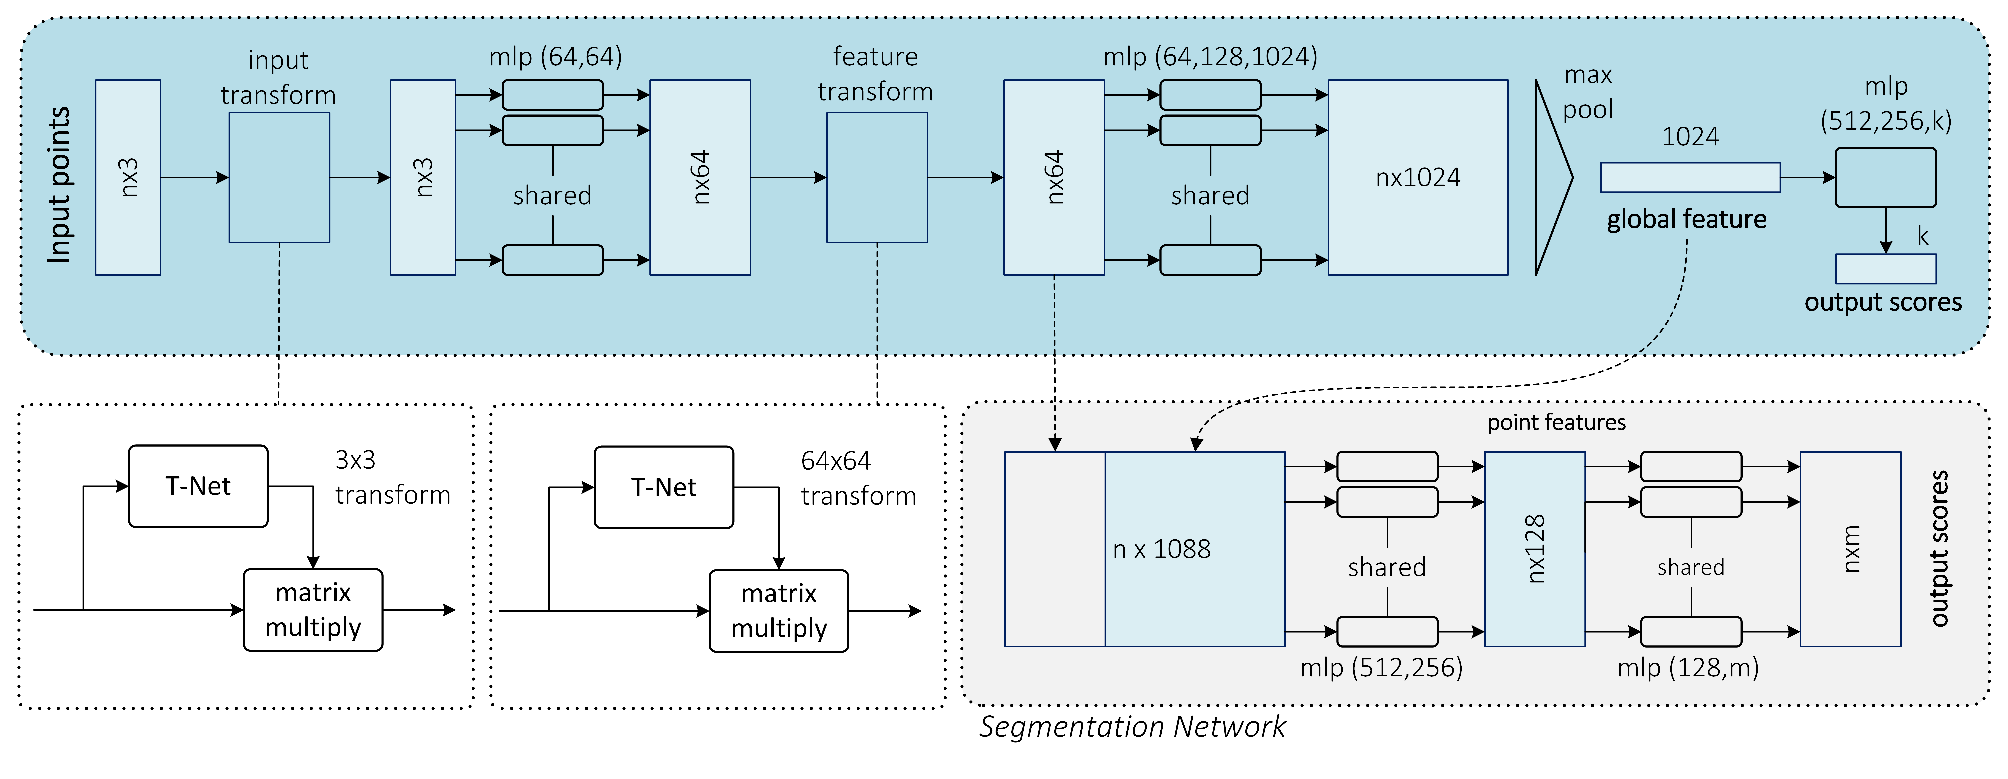
\includegraphics[width=0.9\linewidth]{Figures/Segmentation/pointnetarchitecture_rework}
	\caption{The PointNet unified architecture for point cloud classification and segmentation. Figure reproduced from \cite{Qi2016}.}
	\label{fig:semseg:pointnetarchitecture}
\end{figure*}

Another remarkable work to deal with point clouds as graphs and directly apply convolutions without any kind of discretization is the \ac{DGCNN} \cite{Wang2018}. This novel architecture proposes a new neural network module, namely \emph{EdgeConv}, which operates directly over the point cloud and incorporates several important properties (local neighborhood information, it can be stacked, and it is able to capture long-distance properties). That module is easily pluggable into existing architectures and has been proven to capture and exploit fine-grained and global properties of point clouds expressed as graphs.

\subsection{Video Sequences}

As we have observed, there has been a significant progress in single-image segmentation. However, when dealing with image sequences, many systems rely on the naïve application of the very same algorithms in a frame-by-frame manner. This approach works, often producing remarkable results. Nevertheless, applying those methods frame by frame is usually non-viable due to computational cost. In addition, those methods completely ignore temporal continuity and coherence cues which might help increase the accuracy of the system while reducing its execution time.

Arguably, the most remarkable work in this regard is the clockwork \ac{FCN} by Shelhamer \emph{et al.}\cite{Shelhamer2016}. This network is an adaptation of a \ac{FCN} to make use of temporal cues in video to decrease inference time while preserving accuracy. The clockwork approach relies on the following insight: feature velocity -- the temporal rate of change of features in the network -- across frames varies from layer to layer so that features from shallow layers change faster than deep ones. Under that assumption, layers can be grouped into stages, processing them at different update rates depending on their depth. By doing this, deep features can be persisted over frames thanks to their semantic stability, thus saving inference time. Figure \ref{fig:semseg:clockworkfcn} shows the network architecture of the clockwork \ac{FCN}.

\begin{figure}[!hbt]
	\centering
	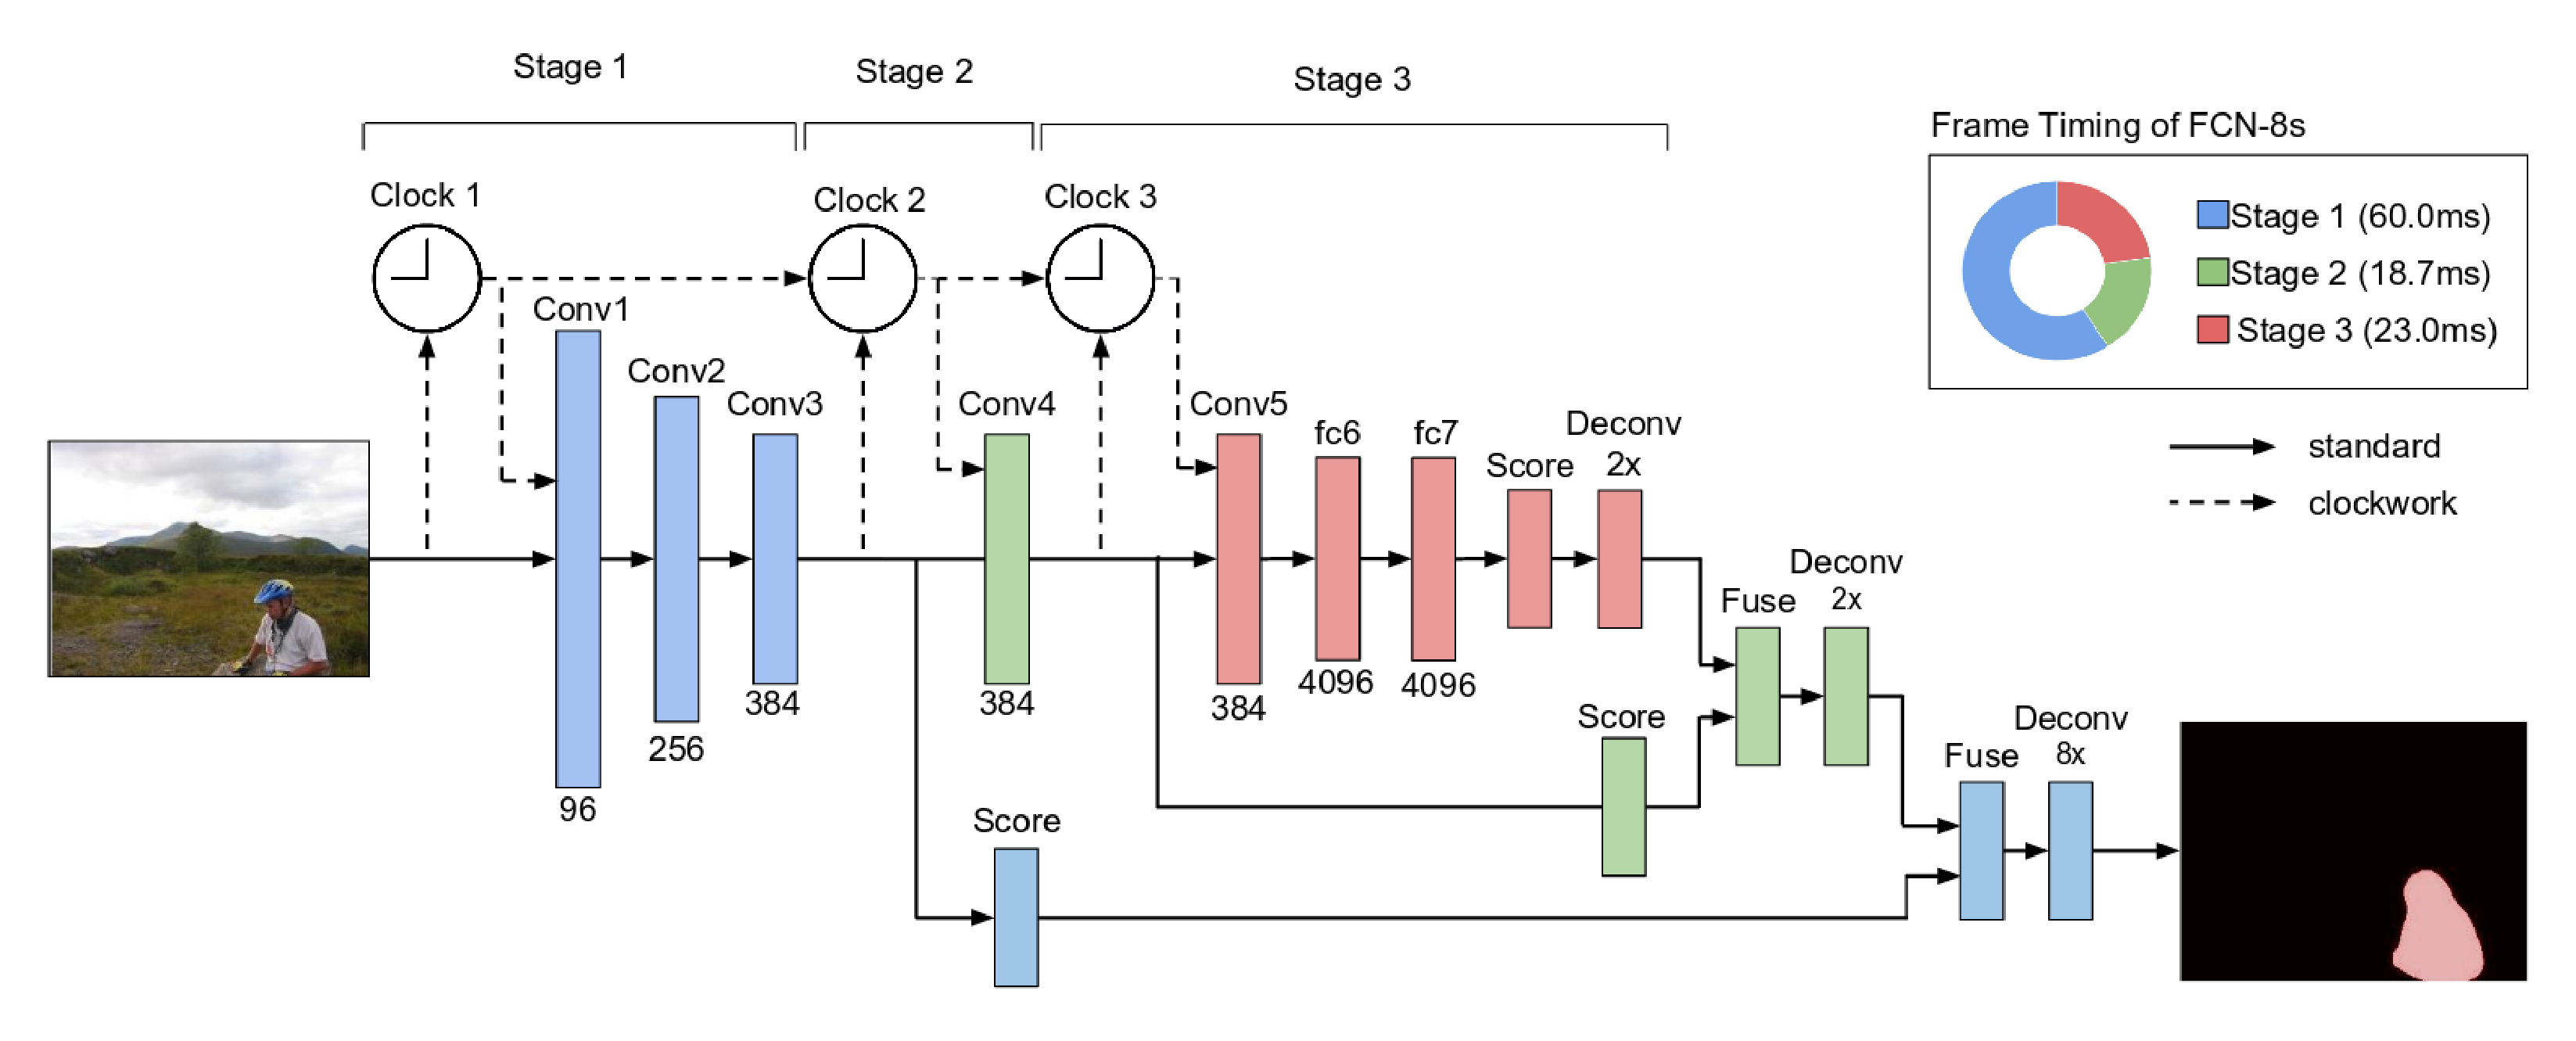
\includegraphics[width=\linewidth]{Figures/Segmentation/clockworkfcn}
	\caption{The clockwork \acs{FCN} with three stages and their corresponding clock rates. Figure extracted from \cite{Shelhamer2016}.}
	\label{fig:semseg:clockworkfcn}
\end{figure}

It is important to remark that the authors propose two kinds of update rates: fixed and adaptive. The fixed schedule just sets a constant time frame for recomputing the features for each stage of the network. The adaptive schedule fires each clock on a data-driven manner, e.g., depending on the amount of motion or semantic change. Figure \ref{fig:semseg:clockworkfcn-adaptive} shows an example of this adaptive scheduling.

\begin{figure}[!hbt]
	\centering
	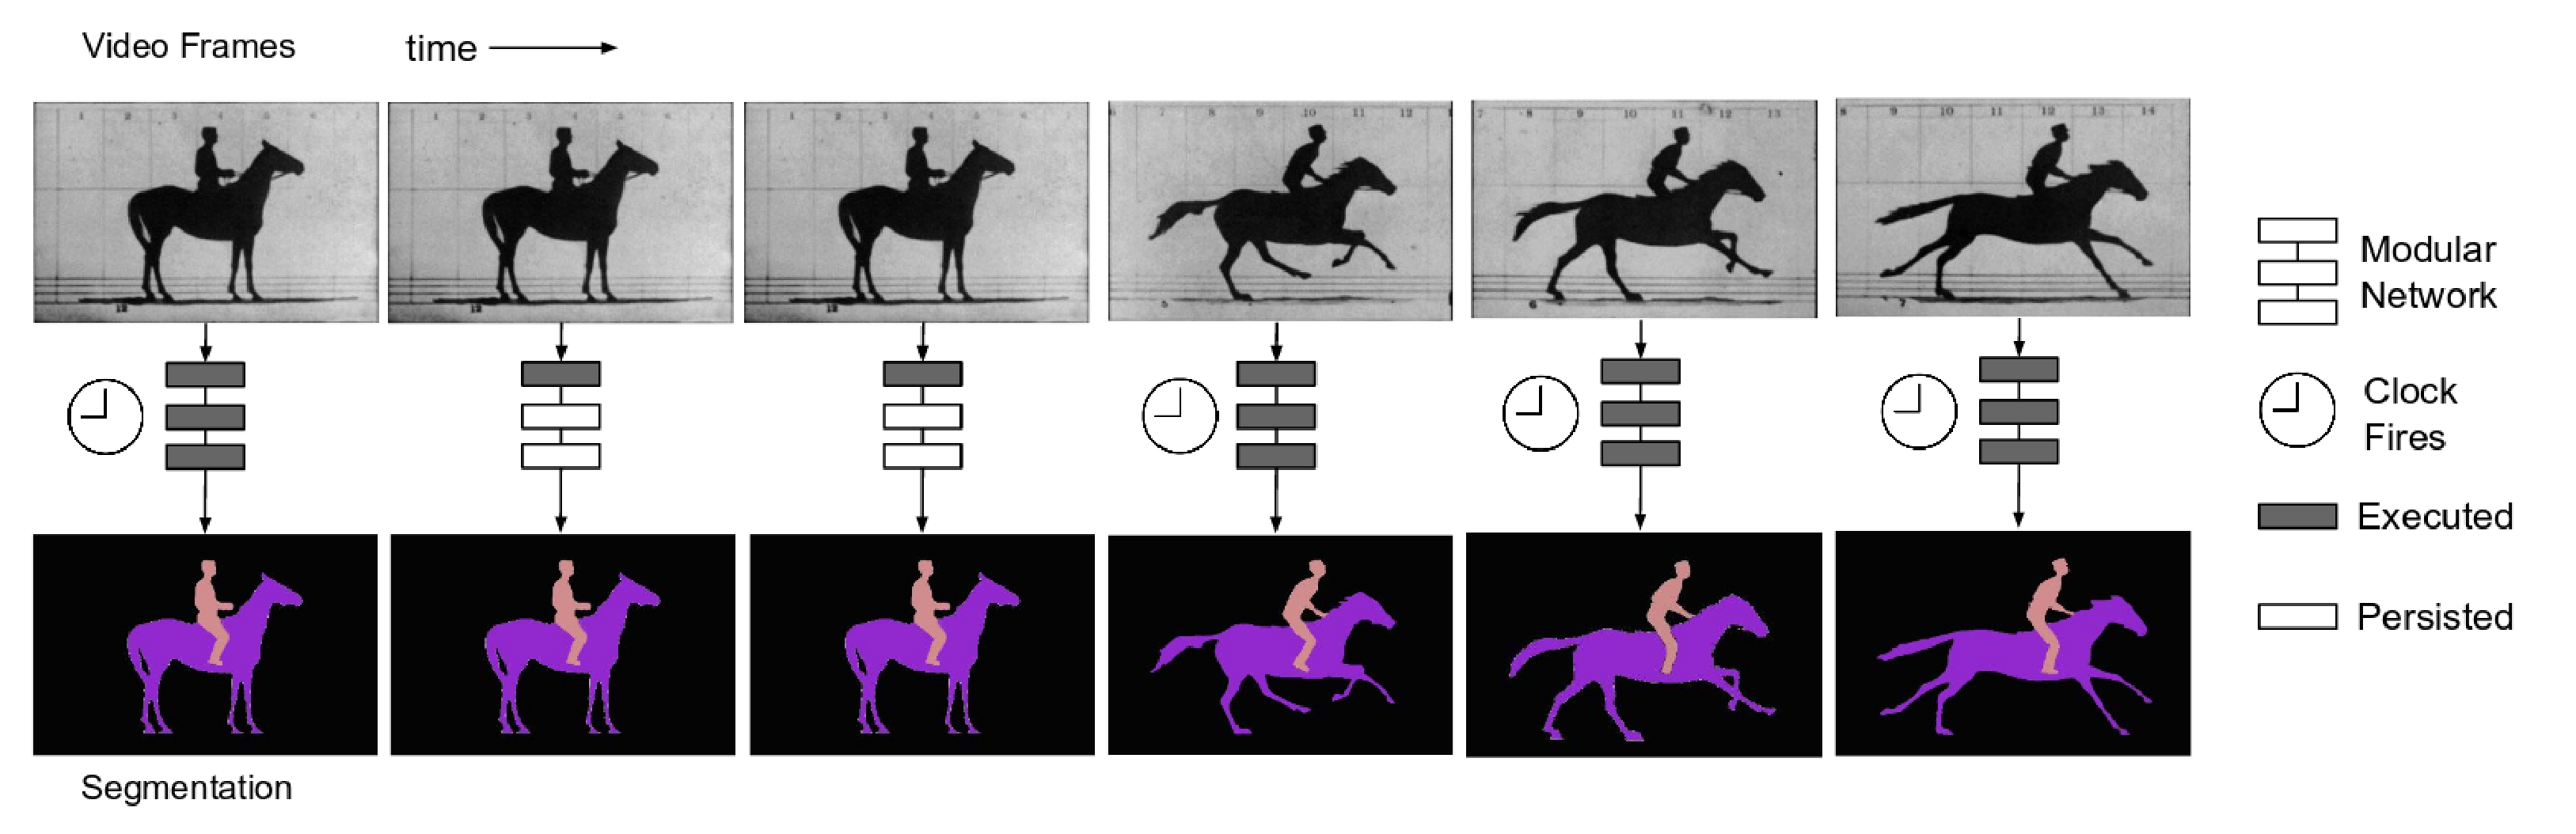
\includegraphics[width=\linewidth]{Figures/Segmentation/clockworkfcn-adaptive}
	\caption{Adaptive clockwork method proposed by Shelhamer \emph{et al.}\cite{Shelhamer2016}. Extracted features persists during static frames while they are recomputed for dynamic ones. Figure extracted from \cite{Shelhamer2016}.}
	\label{fig:semseg:clockworkfcn-adaptive}
\end{figure}

Zhang \emph{et al.}\cite{Zhang2014} took a different approach and made use of a \acs{3D}\acs{CNN}, which was originally created for learning features from volumes, to learn hierarchical spatio-temporal features from multi-channel inputs such as video clips. In parallel, they over-segment the input clip into supervoxels. Then they use that supervoxel graph and embed the learned features in it. The final segmentation is obtained by applying graph-cut\cite{Boykov2001} on the supervoxel graph.

Another remarkable method, which builds on the idea of using 3D convolutions, is the deep end-to-end voxel-to-voxel prediction system by Tran \emph{et al.}\cite{Tran2016}. In that work, they make use of the \ac{C3D} network introduced by themselves on a previous work \cite{Tran2015}, and extend it for semantic segmentation by adding deconvolutional layers at the end. Their system works by splitting the input into clips of $16$ frames, performing predictions for each clip separately. Its main contribution is the use of 3D convolutions. Those convolutions make use of \acl{3D} filters which are suitable for spatio-temporal feature learning across multiple channels, in this case frames. Figure \ref{fig:semseg:2dvs3dconvolutions} shows the difference between 2D and 3D convolutions applied to multi-channel inputs, proving the usefulness of the 3D ones for video segmentation.

\begin{figure}[!hbt]
	\centering
	\begin{subfigure}{0.49\linewidth}
		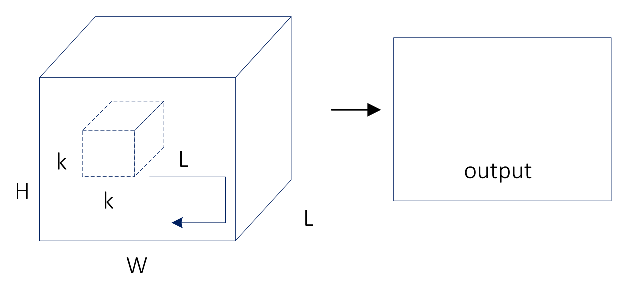
\includegraphics[width=\linewidth]{Figures/Segmentation/2dconvolutionframes.eps}
		\caption{2D Convolution}
		\label{fig:2dvs3dconvolutions:2dconvolution}
	\end{subfigure}
	\hfill
	\begin{subfigure}{0.49\linewidth}
		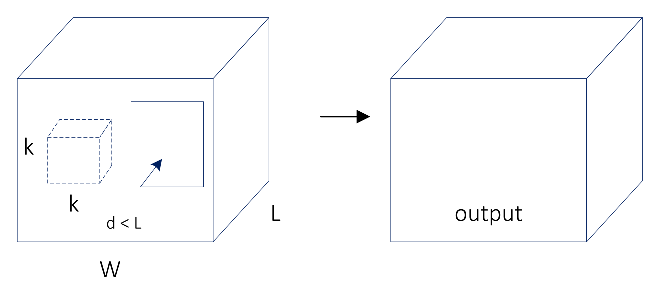
\includegraphics[width=\linewidth]{Figures/Segmentation/3dconvolution.eps}
		\caption{3D Convolution}
		\label{fig:2dvs3dconvolutions:3dconvolution}
	\end{subfigure}
	\caption{Difference between 2D and 3D convolutions applied on a set of frames. (\protect\subref{fig:2dvs3dconvolutions:2dconvolution}) 2D convolutions use the same weights for the whole depth of the stack of frames (multiple channels) and results in a single image. (\protect\subref{fig:2dvs3dconvolutions:3dconvolution}) 3D convolutions use 3D filters and produce a 3D volume as a result of the convolution, thus preserving temporal information of the frame stack.}
	\label{fig:semseg:2dvs3dconvolutions}
\end{figure}

Novel approaches such as \emph{SegmPred} model proposed by Luc et al. \cite{Luc2017} are able to predict semantic segmentation maps of not yet observed video frames in the future. This model consists in a two-scale architecture which is trained in both, adversarial and non-adversarial ways in order to deal with blurred predicted results. Model inputs have been previously per-frame annotated and consists in the softmax output layer pre-activations. Model performance drops when predicting more than a few frames in the future. However, this approach is able to model the object dynamics on the semantic segmentation maps, which remains an open challenge for current computer vision systems.

\subsection{Loss functions for semantic segmentation}

Particular choices of the loss function can strongly affect deep models accuracy and their learning process. For training image and patch-based classification models, we find that the vast majority of research works and applications simply use a cross entropy loss function. However, for regression models, we find that L1 and L2 losses are the most common functions. In this work, we are targeting a slightly different problem, pixel-based classification. An important issue to consider when moving from image or patch-based classification to pixel-based classification is that the last one is more prone to suffer the data imbalance problem. Reviewing existing works in the literature we found that categorical cross entropy and the dice similarity coefficient are the main loss functions used for training semantic segmentation models. We also found different variations for these methods, such as combining both in a weighted manner. For example, ReLayNet \cite{Roy2017} is trained to optimize a joint loss function comprising of weighted categorical cross-entropy and Dice similarity score. Another common variation that has been used in existing works is the use of a weighted scheme for the categorical cross entropy itself. Ronneberger et al \cite{Ronneberger2015} precompute a weight map for the categorical cross entropy loss. It is also very common when we have a single background class and few foreground classes, in that case, the data imbalance problem becomes overwhelming. Several previous approaches resorted to loss functions based on sample re-weighting where foreground regions are given more importance than background ones during learning. However, other approaches only optimize the dice similarity score instead \cite{Milletari2016}. More recently, a new variant has been presented, it is a loss strategy coined as Focal Loss \cite{Lin2017b}, that adds a factor $\gamma$ to the standard cross entropy criterion. It basically reduces the relative loss for well-classified pixels and puts more focus on hard, misclassified ones. A similar strategy can be applied for refining object boundaries, which often contain misclassified pixels.
 
Reviewing loss functions used in existing architectures for semantic segmentation, we find that \ac{FCN} \cite{Long2015} was trained using a per-pixel multinomial logistic loss and was validated with the standard metric of mean pixel intersection over union. The more recent DeepLab \cite{Chen2016} architecture, similarly to \ac{FCN}, uses as a loss function the sum of cross-entropy terms for each spatial position in the \ac{CNN} output map. PSPNet \cite{Zhao2016} also uses the cross-entropy loss function, but in this work, two loss functions are optimized during the training of the network. Apart from the main branch using cross-entropy loss to train the final classifier, another classifier is applied after the fourth stage. The optimization of these two functions is performed in a weighted manner, applying different weights to each loss function and therefore balancing the auxiliary loss function. SegmPred \cite{Luc2017} model relies on \ac{GDL}, designed to sharpen results by penalizing high-frequency mismatches such as errors along the object boundaries. Using \ac{GDL} alongside L1 loss function, SegmPred model results significantly improved by sharpening its outputs. 

In general, the particular choice of the loss function will depend on the type, amount of classes and samples that your dataset contains for each class. Moreover, it is important to consider the number of pixels that are hard to classify pixels in your dataset (compared to the total amount in the ground truth segmentation masks). Based on those aspects, some of the previously presented approaches may help you facing the data imbalance problem and therefore, provide you with a more accurate model for semantic segmentation.

\section{Discussion}
\label{cha:semseg:sec:discussion}

In the previous section we reviewed the existing methods from a literary and qualitative point of view, i.e., we did not take any quantitative result into account. In this Section we are going to discuss the very same methods from a numeric standpoint. First of all, we will describe the most popular evaluation metrics that can be used to measure the performance of semantic segmentation systems from three aspects: execution time, memory footprint, and accuracy. Next, we will gather the results of the methods on the most representative datasets using the previously described metrics. After that, we will summarize and draw conclusions about those results. At last, we enumerate possible future research lines that we consider significant for the field.

\subsection{Evaluation Metrics}

For a segmentation system to be useful and actually produce a significant contribution to the field, its performance must be evaluated with rigor. In addition, that evaluation must be performed using standard and well-known metrics that enable fair comparisons with existing methods. Furthermore, many aspects must be evaluated to assert the validity and usefulness of a system: execution time, memory footprint, and accuracy. Depending on the purpose or the context of the system, some metrics might be of more importance than others, i.e., accuracy may be expendable up to a certain point in favor of execution speed for a real-time application. Nevertheless, for the sake of scientific rigor it is of utmost importance to provide all the possible metrics for a proposed method.

\subsubsection{Execution Time}

Speed or runtime is an extremely valuable metric since the vast majority of systems must meet hard requirements on how much time can they spend on the inference pass. In some cases it might be useful to know the time needed for training the system, but it is usually not that significant, unless it is exaggeratedly slow, since it is an offline process. In any case, providing exact timings for the methods can be seen as meaningless since they are extremely dependant on the hardware and the backend implementation, rendering some comparisons pointless.

However, for the sake of reproducibility and in order to help fellow researchers, it is useful to provide timings with a thorough description of the hardware in which the system was executed on, as well as the conditions for the benchmark. If done properly, that can help others estimate if the method is useful or not for the application as well as perform fair comparisons under the same conditions to check which are the fastest methods.

\subsubsection{Memory Footprint}

Memory usage is another important factor for segmentation methods. Although it is arguably less constraining than execution time -- scaling memory capacity is usually feasible -- it can also be a limiting element. In some situations, such as onboard chips for robotic platforms, memory is not as abundant as in a high-performance server. Even high-end \acp{GPU}, which are commonly used to accelerate deep networks, do not pack a copious amount of memory. In this regard, and considering the same implementation-dependent aspects as with runtime, documenting the peak and average memory footprint of a method with a complete description of the execution conditions can be extraordinarily helpful.

\subsubsection{Accuracy}

Many evaluation criteria have been proposed and are frequently used to assess the accuracy of any kind of technique for semantic segmentation. Those metrics are usually variations on pixel accuracy and \ac{IoU}. We report the most popular metrics for semantic segmentation that are currently used to measure how per-pixel labeling methods perform on this task. For the sake of the explanation, we remark the following notation details: we assume a total of $k+1$ classes (from $L_0$ to $L_{k}$ including a void class or background) and $p_{ij}$ is the amount of pixels of class $i$ inferred to belong to class $j$. In other words, $p_{ii}$ represents the number of true positives, while $p_{ij}$ and $p_{ji}$ are usually interpreted as false positives and false negatives respectively (although either of them can be the sum of both false positives and false negatives)..

\begin{itemize}
	\item \textbf{\ac{PA}}: it is the simplest metric, simply computing a ratio between the amount of properly classified pixels and the total number of them.
		\begin{align*}
			PA = \displaystyle\frac{\displaystyle\sum_{i=0}^k p_{ii}}{\displaystyle\sum_{i=0}^k\displaystyle\sum_{j=0}^k p_{ij}}
		\end{align*}
	\item \textbf{\ac{MPA}}: a slightly improved \ac{PA} in which the ratio of correct pixels is computed in a per-class basis and then averaged over the total number of classes.
		\begin{align*}
			MPA = \displaystyle\frac{1}{k+1}\displaystyle\sum_{i=0}^k \displaystyle\frac{p_{ii}}{\displaystyle\sum_{j=0}^k p_{ij}}
		\end{align*}
	\item \textbf{\ac{MIoU}}: this is the standard metric for segmentation purposes. It computes a ratio between the intersection and the union of two sets, in our case the ground truth and our predicted segmentation. That ratio can be reformulated as the number of true positives (intersection) over the sum of true positives, false negatives, and false positives (union). That \ac{IoU} is computed on a per-class basis and then averaged.
		\begin{align*}
			MIoU = \displaystyle\frac{1}{k+1}\displaystyle\sum_{i=0}^k \displaystyle\frac{p_{ii}}{\displaystyle\sum_{j=0}^k p_{ij} + \displaystyle\sum_{j=0}^k p_{ji} - p_{ii}}
		\end{align*}
	\item \textbf{\ac{FWIoU}}: it is an improved over the raw \ac{MIoU} which weights each class importance depending on their appearance frequency.
		\begin{align*}
			FWIoU = \displaystyle\frac{1}{\displaystyle\sum_{i=0}^k \displaystyle\sum_{j=0}^k p_{ij}} \displaystyle\sum_{i=0}^k \displaystyle\frac{\displaystyle\sum_{j=0}^k p_{ij} p_{ii}}{\displaystyle\sum_{j=0}^k p_{ij} + \displaystyle\sum_{j=0}^k p_{ji} - p_{ii}}
		\end{align*}
\end{itemize}

Of all metrics described above, the \ac{MIoU} stands out of the crowd as the most used metric due to its representativeness and simplicity. Most challenges and researchers make use of that metric to report their results.

\clearpage

\subsection{Results}

As we stated before, Section \ref{cha:semseg:sec:methods} provided a functional description of the reviewed methods according to their targets. Now we gathered all the quantitative results for those methods as stated by their authors in their corresponding papers (see Table \ref{table:semseg:results}. These results are organized into three parts depending on the input data used by the methods: \acs{2D} \acs{RGB} or \acs{2.5D} \acs{RGB-D} images, volumetric \acs{3D}, or video sequences.

The most used datasets have been selected for that purpose. It is important to remark the heterogeneity of the papers in the field when reporting results. Although most of them try to evaluate their methods in standard datasets and provide enough information to reproduce their results, also expressed in widely known metrics, many others fail to do so. That leads to a situation in which it is hard or even impossible to fairly compare methods.

\begin{table}[!htb]
  \centering
  \resizebox{\linewidth}{!}{
  \begin{tabular}{|r|c|c|c|c|c|c|c|||c|c|c|||c|c|||c|}
    \hline
    Method & \rotatebox[origin=c]{90}{PASCAL VOC-2012} & \rotatebox[origin=c]{90}{PASCAL-Context} & \rotatebox[origin=c]{90}{Pascal Person-Part} & \rotatebox[origin=c]{90}{CamVid} & \rotatebox[origin=c]{90}{CityScapes} & \rotatebox[origin=c]{90}{Stanford Background} & \rotatebox[origin=c]{90}{SiftFlow} & \rotatebox[origin=c]{90}{SUN RGB-D} & \rotatebox[origin=c]{90}{NYUDv2} & \rotatebox[origin=c]{90}{SUN3D} & \rotatebox[origin=c]{90}{ShapeNet Part} & \rotatebox[origin=c]{90}{Stanford 2D-3D-S} & \rotatebox[origin=c]{90}{Youtube-Objects}\\
    \hline
    \acs{PSPNet}\cite{Zhao2016} & \textbf{85.40} & - & - & - & \textbf{80.20} & - & - & - & - & - & - & - & -\\
    DeepLab\cite{Chen2016} & 79.70 & \textbf{45.70} & \textbf{64.94} & - & 70.40 & - & - & - & - & - & - & - & -\\
    Dilation-10\cite{Yu2015} & 75.30 & - & - & - & 67.10 & - & - & - & - & - & - & - & -\\
		CRFasRNN\cite{Zheng2015} & 74.70 & 39.28 & - & - & 62.50 & - & - & - & - & - & - & - & -\\
		ParseNet\cite{Liu2015} & 69.80 & - & - & - & - & - & - & - & - & - & - & - & -\\
    \acs{FCN}-8s\cite{Long2015} & 67.20 & 39.10 & - & - & 65.30 & - & - & - & - & - & - & - & -\\
		M.scale-CNN-Eigen\cite{Eigen2015} & 62.60 & - & - & - & - & - & - & - & - & - & - & - & - \\
		Bayesian SegNet\cite{Kendall2015} & 60.50 & - & - & 63.10 & - & - & - & - & - & - & - & - & - \\
    SegNet\cite{Badrinarayanan2015} & - & - & - & 60.10 & - & - & - &- & - & - & - & - & -\\
    DAG-RNN\cite{Shuai2015} & - & - & - & \textbf{91.60} & - & - & \textbf{85.30} & - & - & - & - & - & - \\
    ReSeg \cite{Visin2016} & - & - & - & 58.80 & - & - & - & - & - & - & - & - & - \\
\
    ENet\cite{Paszke2016} & - & - & - & 55.60 & 58.30 & - & - & - & - & - & - & - & - \\
    rCNN\cite{Pinheiro2014} & - & - & - & - & - & \textbf{80.20} & 77.70 & - & - & - & - & - & - \\
    2D-LSTM\cite{Byeon2015} & - & - & - & - & - & 78.56 & 70.11 & - & - & - & - & - & - \\
    \acs{LSTM-CF}\cite{Li2016b} & - & - & - & - & - & - & - & \textbf{48.10} & \textbf{49.40} & \textbf{58.50} & - & - & - \\
    PointNet\cite{Qi2016} & - & - & - & - & - & - & - & - & - & - & \textbf{83.70} & \textbf{47.71} & -\\
    PointNet++\cite{Qi2017} & - & - & - & - & - & - & - & - & - & - & \textbf{85.10} & - & -\\
    \ac{DGCNN}\cite{Wang2018} & - & - & - & - & - & - & - & - & - & - & \textbf{85.10} & \textbf{56.10} & -\\
    Clockwork Convnet\cite{Shelhamer2016} & - & - & - & - & \textbf{64.40} & - & - & - & - & - & - & - & \textbf{68.50} \\
    SegmPred \cite{Luc2017} \footnote{This model is focused on predicting future frames in the space of semantic segmentation, thus a direct comparison with the other methods listed in this table would not be fair.} & - & - & - & \textbf{46.80} & \textbf{59.40} & - & - & - & - & - & - & - & - \\
    \hline
  \end{tabular}}
  \caption{Accuracy results for the most relevant methods and datasets.}
  \label{table:semseg:results}
\end{table}

Furthermore, we also came across the fact few authors provide information about other metrics rather than accuracy. Despite the importance of other metrics, most of the papers do not include any data about execution time nor memory footprint. In some cases that information is provided, but no reproducibility information is given so it is impossible to know the setup that produced those results which are of no use.

\subsubsection{\acs{RGB}}

For the single \acs{2D} image category we have selected seven datasets: PASCAL \acs{VOC}2012, PASCAL Context, PASCAL Person-Part, CamVid, CityScapes, Stanford Background, and SiftFlow. That selection accounts for a wide range of situations and targets.

The first, and arguably the most important dataset, in which the vast majority of methods are evaluated is PASCAL \acs{VOC}-2012. This set of results shows a clear improvement trend from the firs proposed methods (SegNet and the original \acs{FCN}) to the most complex models such as \acs{CRF}as\acs{RNN} and the winner (\acs{PSPNet}) with $85.70$ \acs{IoU}.

Apart from the widely known \acs{VOC} we also collected metrics of its Context counterpart in which DeepLab is the top scorer ($45.70$ \acs{IoU}).

In addition, we also took into account the PASCAL Part dataset. In this case, the only analyzed method that provided metrics for this dataset is DeepLab which achieved a $64.94$ \acs{IoU}.

Moving from a general-purpose dataset such as PASCAL \acs{VOC}, we also gathered results for two of the most important urban driving databases. For CamVid, an \acs{RNN}-based approach (DAG-\acs{RNN}) is the top one with a $91.60$ \acs{IoU}. Results on a more challenging and currently more in use database like CityScapes change. The trend on this dataset is similar to the one with PASCAL \acs{VOC} with \acs{PSPNet} leading with a $80.20$ \acs{IoU}.

The results of various recurrent networks on the Stanford Background dataset are also remarkable. The winner, r\acs{CNN}, achieves a maximum accuracy of $80.20$ \acs{IoU}.

At last, results for another popular dataset such as SiftFlow are also dominated by recurrent methods. In particular DAG-\acs{RNN} is the top scorer with $85.30$ \acs{IoU}.

\subsubsection{\acs{2.5D}}

Regarding the \acs{2.5D} category, i.e., datasets which also include depth information apart from the typical \acs{RGB} channels, we have selected three of them for the analysis: SUN-\acs{RGB-D} and NYUDv2. Results for SUN-\acs{RGB-D} are only provided by \acs{LSTM-CF}, which achieves $48.10$ \acs{IoU}. In the case of NYUDv2, results are exclusive too for \acs{LSTM-CF}. That method reaches $49.40$ \acs{IoU}. \acs{LSTM-CF} is the only one which provides information for SUN-3D, in this case a $58.50$ accuracy.

\subsubsection{\acs{3D}}

Two \acs{3D} datasets have been chosen for this discussion: ShapeNet Part and Stanford-\acs{2D}-\acs{3D}-S. PointNet++ and \ac{DGCNN} are the most promising alternatives in part segmentation with $85.10$ mean \ac{IoU}. In the case of Stanford-\acs{2D}-\acs{3D}-S, \ac{DGCNN} raised the bar set by PointNet from $47.71$ to $56.10$ mean \ac{IoU}.

\subsubsection{Sequences}

The last category included in this discussion is video or sequences. For that part we gathered results for two datasets which are suitable for sequence segmentation: CityScapes and YouTube-Objects. Only one of the reviewed methods for video segmentation provides quantitative results on those datasets: Clockwork Convnet. That method reaches $64.40$ \acs{IoU} on CityScapes, and $68.50$ on YouTube-Objects.

\subsection{Summary}

In light of the results, we can draw various conclusions. The most important of them is related to reproducibility. As we have observed, many methods report results on non-standard datasets or they are not even tested at all. That makes comparisons impossible. Furthermore, some of them do not describe the setup for the experimentation or do not provide the source code for the implementation, thus significantly hurting reproducibility. Methods should report their results on standard datasets, exhaustively describe the training procedure, and also make their models and weights publicly available to enable progress.

Another important fact discovered thanks to this study is the lack of information about other metrics such as execution time and memory footprint. Almost no paper reports this kind of information, and those who do suffer from the reproducibility issues mentioned before. This void is due to the fact that most methods focus on accuracy without any concern about time or space. However, it is important to think about where are those methods being applied. In practice, most of them will end up running on embedded devices, e.g., self-driving cars, drones, or robots, which are fairly limited from both sides: computational power and memory.

Regarding the results themselves, we can conclude that DeepLab is the most solid method which outperforms the rest on almost every single \acs{RGB} images dataset by a significant margin. The \acs{2.5D} or multimodal datasets are dominated by recurrent networks such as \acs{LSTM-CF}. \acs{3D} data segmentation still has a long way to go with PointNet paving the way for future research on dealing with unordered point clouds without any kind of preprocessing or discretization. Finally, dealing with video sequences is another green area with no clear direction, but Clockwork Convnets are the most promising approach thanks to their efficiency and accuracy duality. \acs{3D} convolutions are worth remarking due to their power and flexibility to process multichannel inputs, making them successful at capturing both spatial and temporal information.

\subsection{Future Research Directions}

Based on the reviewed research, which marks the state of the art of the field, we present a list of future research directions that would be interesting to pursue.

\begin{itemize}
	\item \emph{3D datasets}: methods that make full use of \acs{3D} information are starting to rise but, even if new proposals and techniques are engineered, they still lack one of the most important components: data. There is a strong need for large-scale datasets for \acs{3D} semantic segmentation, which are harder to create than their lower dimensional counterparts. Although there are already some promising works, there is still room for more, better, and varied data. It is important to remark the importance of real-world 3D data since most of the already existing works are synthetic databases. A proof of the importance of \acs{3D} is the fact that the \acs{ILSVRC} will feature \acs{3D} data in 2018.
	\item \emph{Sequence datasets}: the same lack of large-scale data that hinders progress on \acs{3D} segmentation also impacts video segmentation. There are only a few datasets that are sequence-based and thus helpful for developing methods which take advantage of temporal information. Bringing up more high-quality data from this nature, either \acs{2D} or \acs{3D}, will unlock new research lines without any doubt.
	\item \emph{Point cloud segmentation using \acp{GCN}}: as we already mentioned, dealing with \acs{3D} data such as point clouds poses an unsolved challenge. Due to its unordered and unstructured nature, traditional architectures such as \acp{CNN} cannot be applied unless some sort of discretization process is applied to structure it. One promising line of research aims to treat point clouds as graphs and apply convolutions over them \cite{Henaff2015} \cite{Kipf2016} \cite{Niepert2016}. This has the advantage of preserving spatial cues in every dimension without quantizing data.
	\item \emph{Context knowledge}: while \acp{FCN} are a consolidated approach for semantic segmentation, they lack several features such as context modelling that help increasing accuracy. The reformulation of CRFs as RNNs to create end-to-end solutions seems to be a promising direction to improve results on real-life data. Multi-scale and feature fusion approaches have also shown remarkable progress. In general, all those works represent important steps towards achieving the ultimate goal, but there are some problems that still require more research.
	\item \emph{Real-time segmentation}: In many applications, precision is important; however, it is also crucial that these implementations are able to cope with common camera frame rates (at least 25 frames per second). Most of the current methods are far from that framerate, e.g., \acs{FCN}-8s takes roughly $100$ ms to process a low-resolution PASCAL \acs{VOC} image whilst \acs{CRF}as\acs{RNN} needs more than $500$ ms. Therefore, during the next years, we expect a stream of works coming out, focusing more on real-time constraints. These future works will have to find a trade-off between accuracy and runtime.
	\item \emph{Memory:} some platforms are bounded by hard memory constraints. Segmentation networks usually do need significant amounts of memory to be executed for both inference and training. In order to fit them in some devices, networks must be simplified. While this can be easily accomplished by reducing their complexity (often trading it for accuracy), another approaches can be taken. Pruning is a promising research line that aims to simplify a network, making it lightweight while keeping the knowledge, and thus the accuracy, of the original network architecture \cite{Anwar2015}\cite{Han2015}\cite{Molchanov2016}.
	\item \emph{Temporal coherency on sequences:} some methods have addressed video or sequence segmentation but either taking advantage of that temporal cues to increase accuracy or efficiency. However, none of them have explicitly tackled the coherency problem. For a segmentation system to work on video streams it is important, not only to produce good results frame by frame, but also make them coherent through the whole clip without producing artifacts by smoothing predicted per-pixel labels along the sequence.
	\item \emph{Multi-view integration:} Use of multiple views in recently proposed segmentation works is mostly limited to RGB-D cameras and in particular focused on single-object segmentation.
\end{itemize}

\section{Conclusion}
\label{cha:semseg:sec:conclusion}

To the best of our knowledge, this is the first review in the literature which focuses on semantic segmentation using deep learning. In comparison with other surveys, this review is devoted to such a rising topic as deep learning, covering the most advanced and recent work on that front.

We formulated the semantic segmentation problem and provided the reader with the necessary background knowledge about deep learning for the task. We covered the contemporary literature of datasets and methods, providing a comprehensive survey of $28$ datasets and $29$ methods.

Datasets were carefully described, stating their purposes and characteristics so that researchers can easily pick the one that best suits their needs. We presented a comparative summary of datasets in a tabular form to ease the comparison.

Methods were surveyed from two perspectives: contributions (from a result-agnostic point of view) and raw results, i.e., accuracy (quantitative evaluation on the most common datasets). We also presented a comparative summary of methods in tabular form and grouped them hierarchically in a graph.

In the end, we discussed the results and provided useful insight for future research directions and open problems in the field. A general conclusion that we can draw from this study is that semantic segmentation has been approached with many success stories but still remains an open problem whose solution would prove really useful for a wide set of real-world applications. Furthermore, deep learning has proved to be extremely powerful to tackle this problem so we can expect a flurry of innovation and spawns of research lines in the upcoming years.

\chapter{Sim-2-Real}
\label{cha:sim2real}

\begin{chapterabstract}
    \lipsum[2]
\end{chapterabstract}

\clearpage

\section{Introduction}
\label{cha:sim2real:sec:introduction}

\chapter{Grasp Stability Prediction}
\label{cha:tactile}

\begin{chapterabstract}
    \lipsum[2]
\end{chapterabstract}

\minitoc

\clearpage

\section{Introduction}
\label{cha:tactile:sec:introduction}

\begin{figure}[!b]
	\centering
	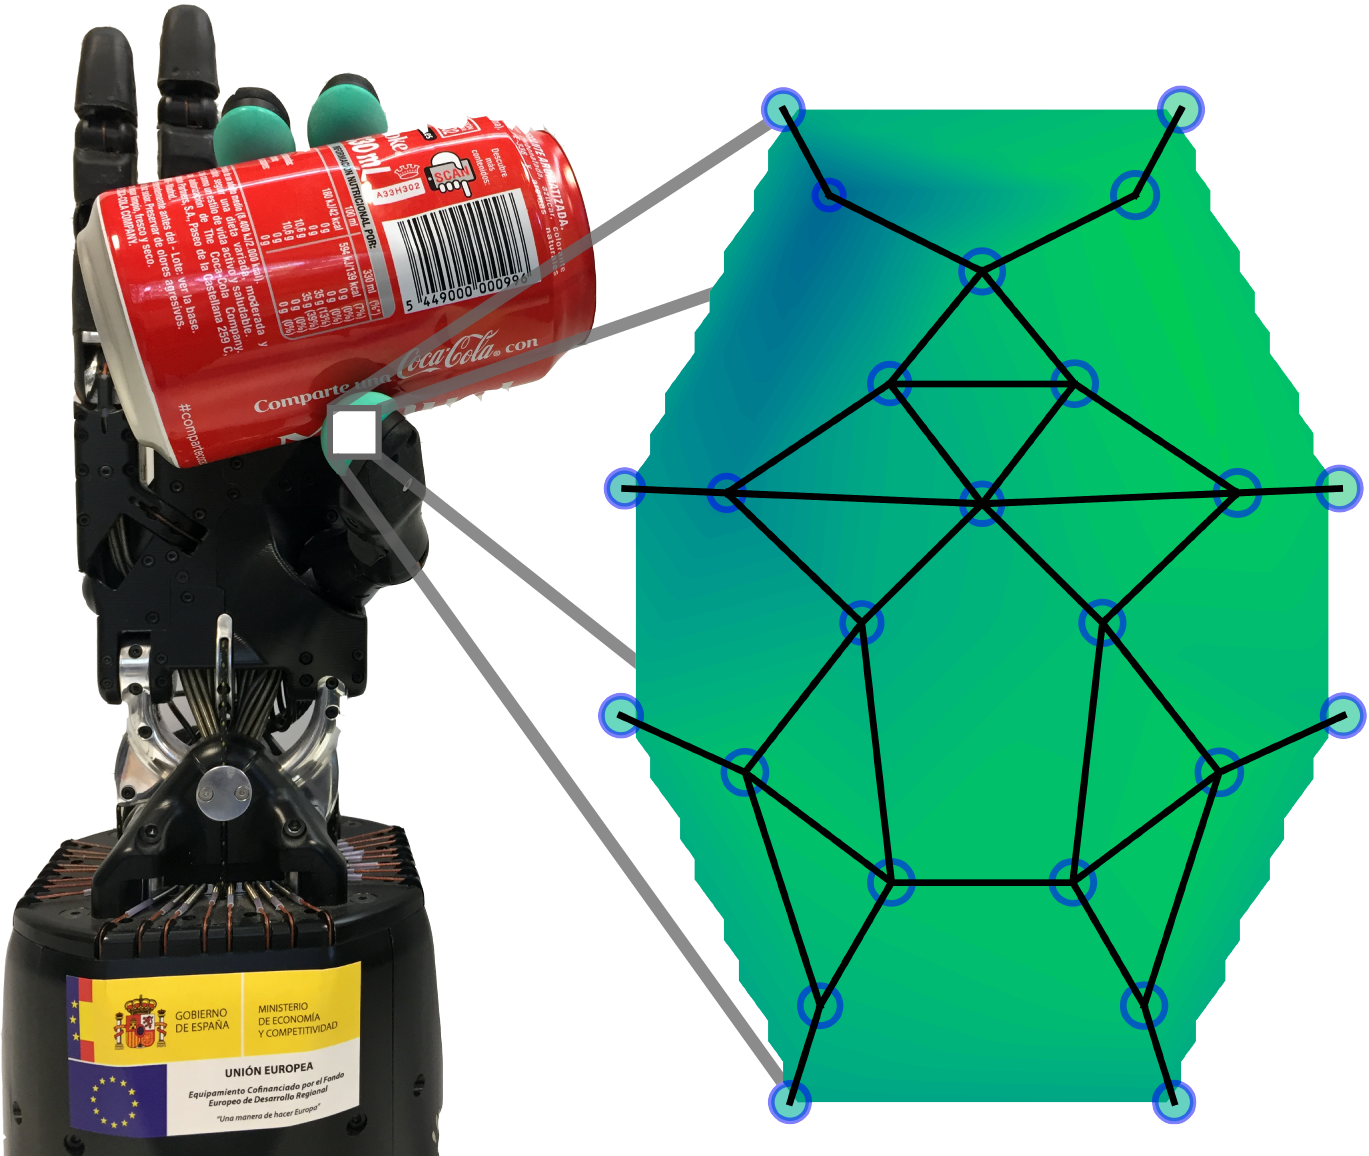
\includegraphics[width = 0.64\textwidth, clip = false, trim = 0 0 0 0]{Figures/Tactile/hand-coke.png}
	\caption{In our proposed TactileGCN framework, we use a Shadow Dexterous hand equipped with three BioTacSP tactile sensors whose readings are transformed into graph representations. Those graphs are then fed as input to a \ac{GCN} in order to learn to predict grasp stability. Figure created by Brayan S. Zapata-Impata and included with his permission.}
	\label{fig:shadow-coke}
\end{figure}

When we humans grasp objects, we intuitively know whether the grip is stable or not even before lifting or manipulating the object. It is not necessary for us to raise our hands or apply any force (either direct such as hitting the object or either indirect such as gravity) in order to determine the object will remain stable between our fingers or our palms. By leveraging our tactile sense, along with our vision and all our intuition and years of experience, we can accurately predict the stability of the grasp for a variety of objects in a wide range of situations. This skill is desirable for any robotic manipulator since it favors the early detection of grasp failures so the robot can react as quick as possible. For instance, a restocking robot working in a store would recognize when an object could slip from its hand and react accordingly and swiftly to avoid a situation in which the object would fall and possibly break down. However easy this task is for a human being, it is not anywhere near as obvious for a robot: there are simply too many variables to take into account for a straightforward solution, e.g., the object's weight, roughness, and geometry; the force of gravity; and the momentum that the object may if we move it to name a few.

The problem of predicting the stability of a grasp is a challenging and ongoing research topic in the field of robotics. The vast majority of the literature, which will be reviewed in depth later in this chapter, makes use of tactile sensors as the main source of data since they provide valuable and abundant information (e.g., temperature or pressure) about the forces that act during the interaction of the robotic hand with the objects \cite{Kappassov2015}. Although methods, datasets, and sensors vary across existing works, all of them agree to distinguish two different states for the grasp: stable, meaning that the object is firmly grasped; or slippery, which means that the object could slide from the hand.

Previous works found in the literature approach this problem following the next methodology: grasp the object, read the tactile sensors equipped in the fingers and/or palm of the hand, calculate custom features that try to characterize these two stability states and learn them in order to make future predictions \cite{Li2014b,Dang2014,Su2015b,Veiga2015}. These proposals treat the tactile readings as classic signals: they preprocess them as if they were arrays, calculate features and learn their characteristics using probabilistic methods. As a consequence, their performance highly depends on the selected characteristics. Moreover, the spatial distribution inherent to the tactile sensor is lost due to the fact of squeezing the data into a one dimensional array.

In this chapter, we propose the use of \acp{GNN} for predicting grasp stability. Since these are deep learning models, there is no need to hand-engineer features because the algorithm is designed for learning them by itself. Moreover, graphs can reflect more accurately the real distribution of the electrodes in the sensor as well as their spatial relationships, which should be of great value for learning tactile features. The main contributions of this chapter can be summarized as follows:

\begin{itemize}
	\item We process tactile readings using a novel perspective: instead of considering them as 1D arrays or 2D images, we build a 3D graph connecting the multiple sensing points (taxels) of the tactile sensor.

	\item We introduce a novel way of processing such information using \acfp{GNN}.
	
	\item We quantitatively check the performance of this new methodology in the real world using a set of tactile sensors installed in a robotic hand.

	\item We release an extension that effectively doubles the size of an already existing dataset \cite{Zapata2018} for grasp stability prediction and includes a whole new split for testing.
\end{itemize}

\clearpage

\section{Background}

In order for the reader to properly understand the following information, we provide brief descriptions of two of the most important concepts introduced in this chapter: tactile sensors and \aclp{GNN}. We suggest the well-versed reader to skip the upcoming sections and move on directly onto the literature review in Section \ref{cha:tactile:sec:relatedworks}.

\subsection{Tactile Sensors}

A tactile sensor is a device which is able to measure information that arises from the phyisical interaction with the environment. Most of this kind of sensors are usually modeled or at least loosely inspired by the biological sense of touch: the cutaneous receptors found in the dermis or epidermis which are able to detect stimuli from pain (nociceptors), chemical substances (chemoreceptors), temperature (thermoreceptors), and mechanical stimulation (mechanoreceptors). From all those kind of receptors, mechanoreceptors and thermoreceptors are the most common in artificial tactile sensors used in robotics and computer hardware. Thanks to those receptors, robots can complement vision systems by leveraging additional information received when the object is being grasped. Although the progress made in learning algorithms can certainly lead to robots being able to predict mechanical properties of the objects, e.g., weight, texture, or stiffness, using vision alone, it is not an effective approach for the time being. However, by taking advantage of tactile sensing when interacting with the object, all those properties can be determined with higher success rates.

Tactile sensors for robotics come in different shapes and sizes featuring a wide range of technologies which includes elastoresistive, capacitive, piezoresistive, and even piezoelectric sensors \cite{Dahiya2012}. Arguably, the most common kind of tactile sensors for robotics are the pressure sensor arrays.

Pressure sensor arrays consist of a grid of tactile elements, also known as \emph{tactels}, each one of them being able of providing pressure or force information when objects contact with them or with the sensor at large. One of the most representative examples of such kind of arrays is the BioTac: a finger-like biomimetic tactile sensor which consist of an array of $19$ impedance sensing electrodes in a rigid core that is immersed in an incompressible and conductive liquid which is in turn surrounded by an elastic skin. It works by detecting the impedance changes on the surface of the rigid core as a result of displacements in the liquid when grasping an object (see Figure \ref{fig:tactile:biotac_sensor}).

\begin{figure}[!thb]
    \centering
    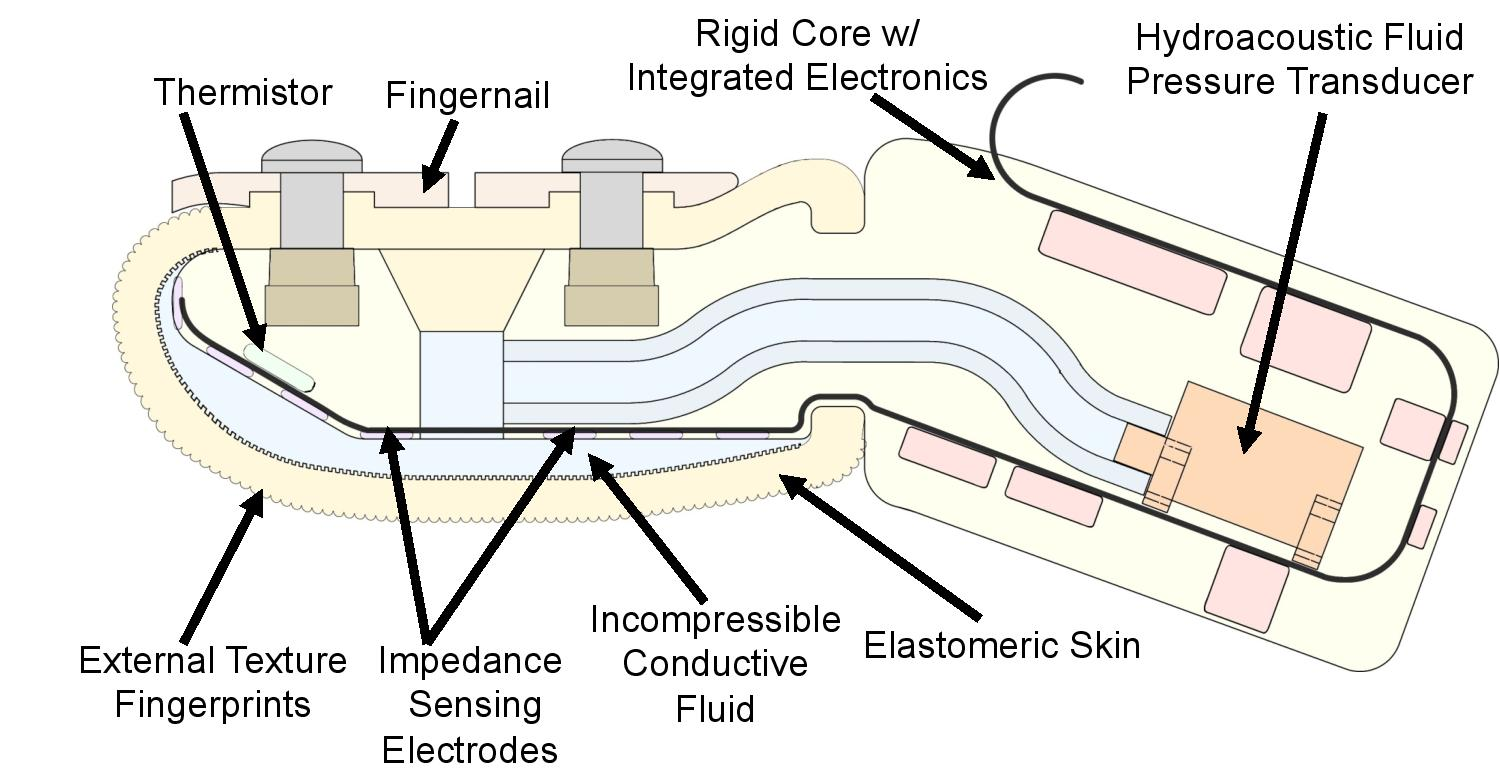
\includegraphics[width=0.65\linewidth]{Figures/Tactile/biotac_1}
    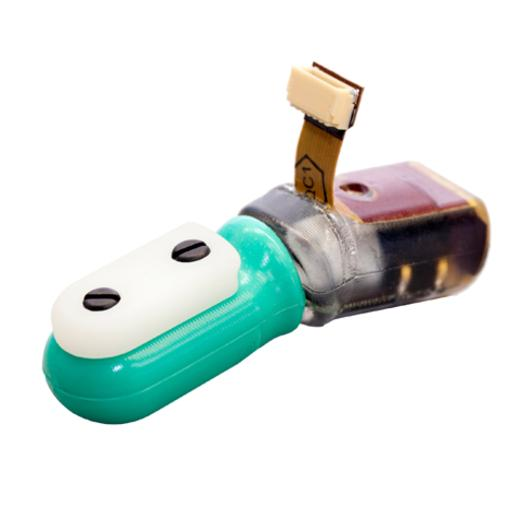
\includegraphics[width=0.34\linewidth]{Figures/Tactile/biotac_2}
    \caption{Cross-section of a BioTac sensor \cite{Syntouch2018} and the actual finger-like product. We can observe how the array of impedance sensing electrodes or tactels are housed in a rigid core which integrates a hydrocoustid fluid pressure transducer as well as a thermistor. The whole package is surrounded by an external and elastomeric skin with external texture fingerprints. The incompressible conductive field is located between the skin and the tactels in the rigid core.}
    \label{fig:tactile:biotac_sensor}
\end{figure}

It is important to remark that the BioTac sensor is also able to provide temperature and heat flow information thanks to a thermistor on the surface of the rigid core that houses the tactels. In this work, we will make use of a more advanced version of the BioTac sensor which will introduced later in the appropriate proposal section.

\subsection{Graph Neural Networks}

Graph data has been an extremely useful representation for such domains in which it is important not only to define features for the elements themselves but also to provide rich information about the connections that relate them. Some of the domains that can take advante of such kind of data are: document analysis, protein folding, physics systems modeling, and social networks to name a few. Usually the tasks that are carried out when analyzing or learning on graphs are node classification or regression, link prediction, and clustering \cite{Zhou2018}. Lately, graph analysis has achieved even more impact not only due to the aforementioned applications but also to the reformulation of data that traditionally belonged to other domains, e.g., natural language processing or image understanding, as graph-like structures. Most of those cases take advantage of the fact that graph representations are able to properly capture non-Euclidean domains. Figure \ref{fig:tactile:graph_applications} shows examples of various graph representations for different domains.

\begin{figure}[!thb]
    \centering
    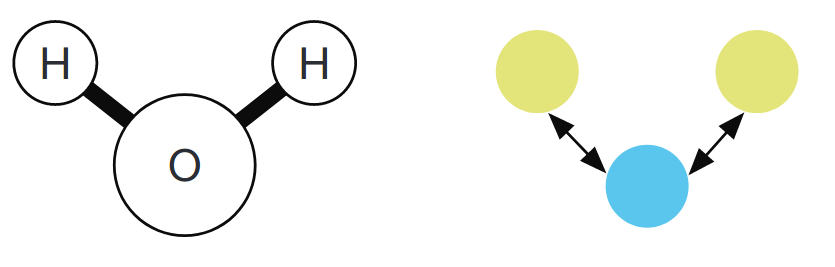
\includegraphics[width=0.49\linewidth]{Figures/Tactile/molecule.png}
    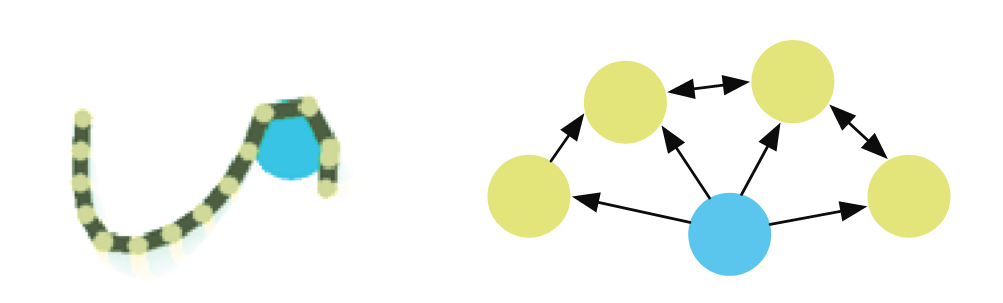
\includegraphics[width=0.49\linewidth]{Figures/Tactile/mass-spring.png}
    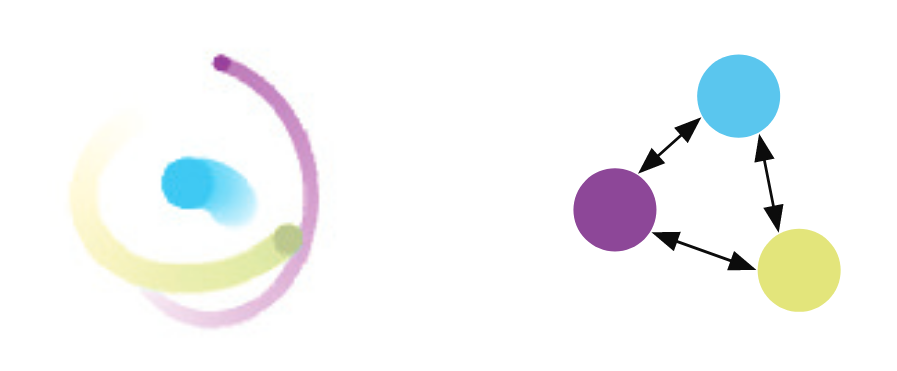
\includegraphics[width=0.49\linewidth]{Figures/Tactile/n-body.png}
    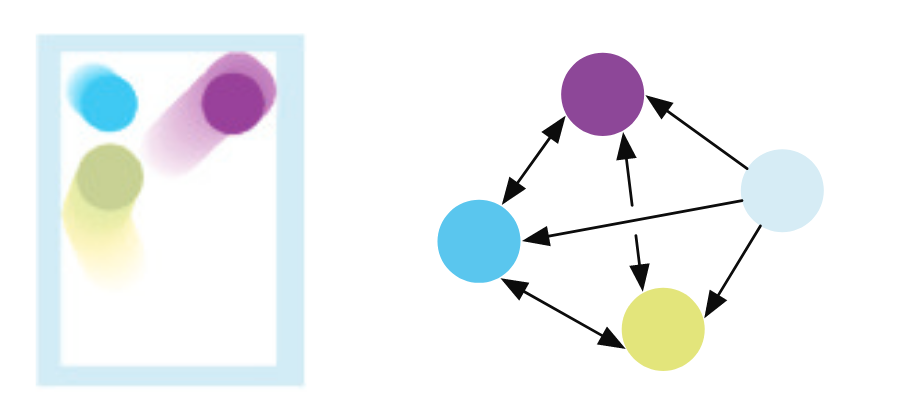
\includegraphics[width=0.49\linewidth]{Figures/Tactile/rigid-body.png}
    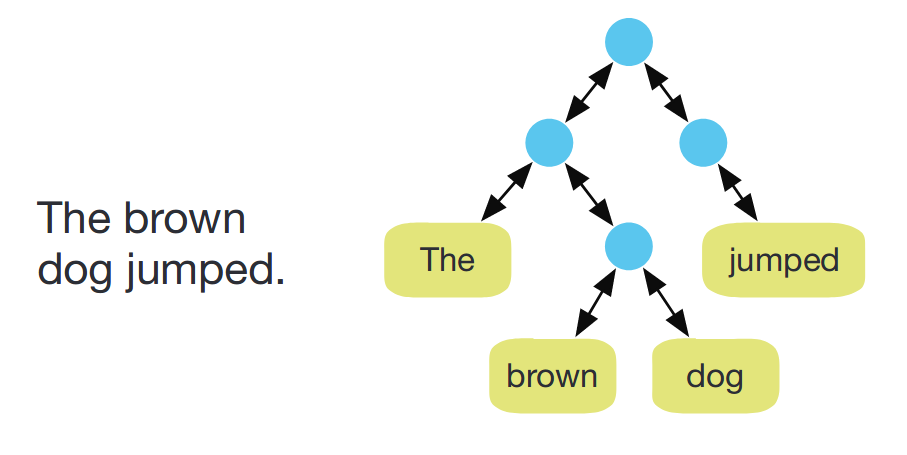
\includegraphics[width=0.49\linewidth]{Figures/Tactile/sentence.png}
    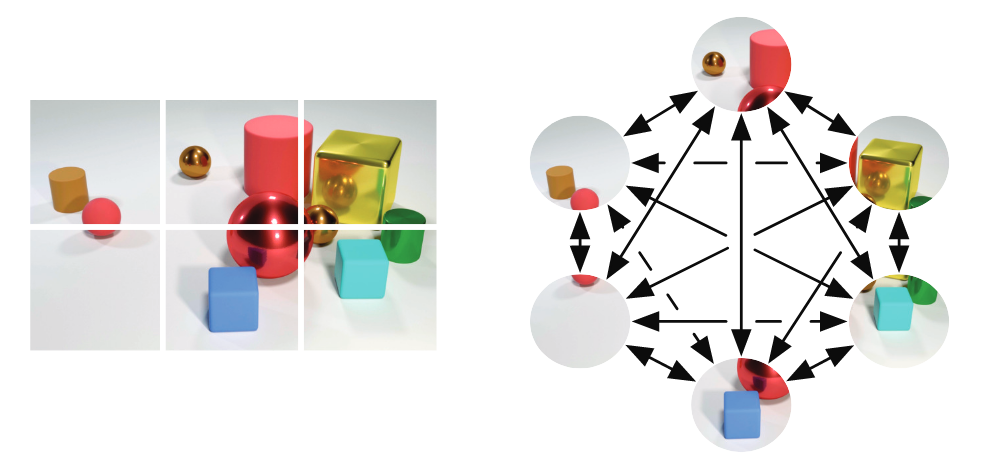
\includegraphics[width=0.49\linewidth]{Figures/Tactile/scene.png}
    \caption{Different graph representations for non-Euclidean domains: a molecule in which each atom is a node and each bond is an edge, a mass-spring system in which the rope is defined by a sequence of masses represented as nodes in the graph, an $n$-body system in which the nodes are the bodies, a rigid-body system, a sentence which can be decomposed into a tree with words as leaves, and a scene-graph which represents a partitioned image and its connections. Figure extracted from \cite{Battaglia2018}.}
    \label{fig:tactile:graph_applications}
\end{figure}

However, despite the usefulnes of graph representations, common and successful architectures such as \aclp{CNN} are not able to deal with non-Euclidean data. As a matter of fact, \acp{CNN} are only able to operate on regular and structured Euclidean representations such as images (\acs{2D} grids) or voxel grids (\acs{3D} grids). Therefore, it is not straightforward to generalize other fruitful architectures such as the \ac{CNN} to graphs mainly due to two reasons: it is hard to define localized filters and pooling operations are not trivial \cite{Zhou2018}.

\acfp{GNN} aim to bridge this gap: they are deep learning architectures which are able to operate directly on non-Euclidean graph domains. The foundations of \acp{GNN} were introduced by Scarselli \emph{et al.} \cite{Scarselli2008} as an extension of traditional neural networks for processing graph data. In this chapter, we will focus on a particular \ac{GNN} architecture that extends the traditional \ac{CNN} one to support operations on graph data: the \acf{GCN}. More details about this architecture will be provided later.

\section{Literature Review}
\label{cha:tactile:sec:relatedworks}

In this section, we review the state of the art of the three main pillars of our work: firstly, we describe previous approaches for predicting grasp stability; secondly, we go through existing datasets which can be used for training grasp stability prediction systems; at last, we explain the most recent and relevant advances in neural networks for graph processing.

\subsection{Grasp Stability Prediction}
\label{cha:tactile:sec:relatedworks:subsec:grasp-stability-prediction}

In the last years, deep learning models have been successfully applied to the problem of grasp stability prediction using tactile sensors as input.

One of the first approaches was taken by Meier \emph{et al.} \cite{Meier2016a}. In this work, they used two piezo-resistive tactile sensor arrays (see Figure \ref{fig:tactile:meier2016}) whose readings were processed to calculate short-time Fourier transforms over a certain window size for each tactel. In this way, they generate spatially arranged stacks of Fourier coefficients to integrate spatial and temporal information in an image-like representation with multiple channels. Then, a \ac{CNN} trained with these matrices is used to predict grasp stability for a dataset of three objects. Furthermore, they also discriminate between rotational and translational slippage.

\begin{figure}[!htb]
    \centering
    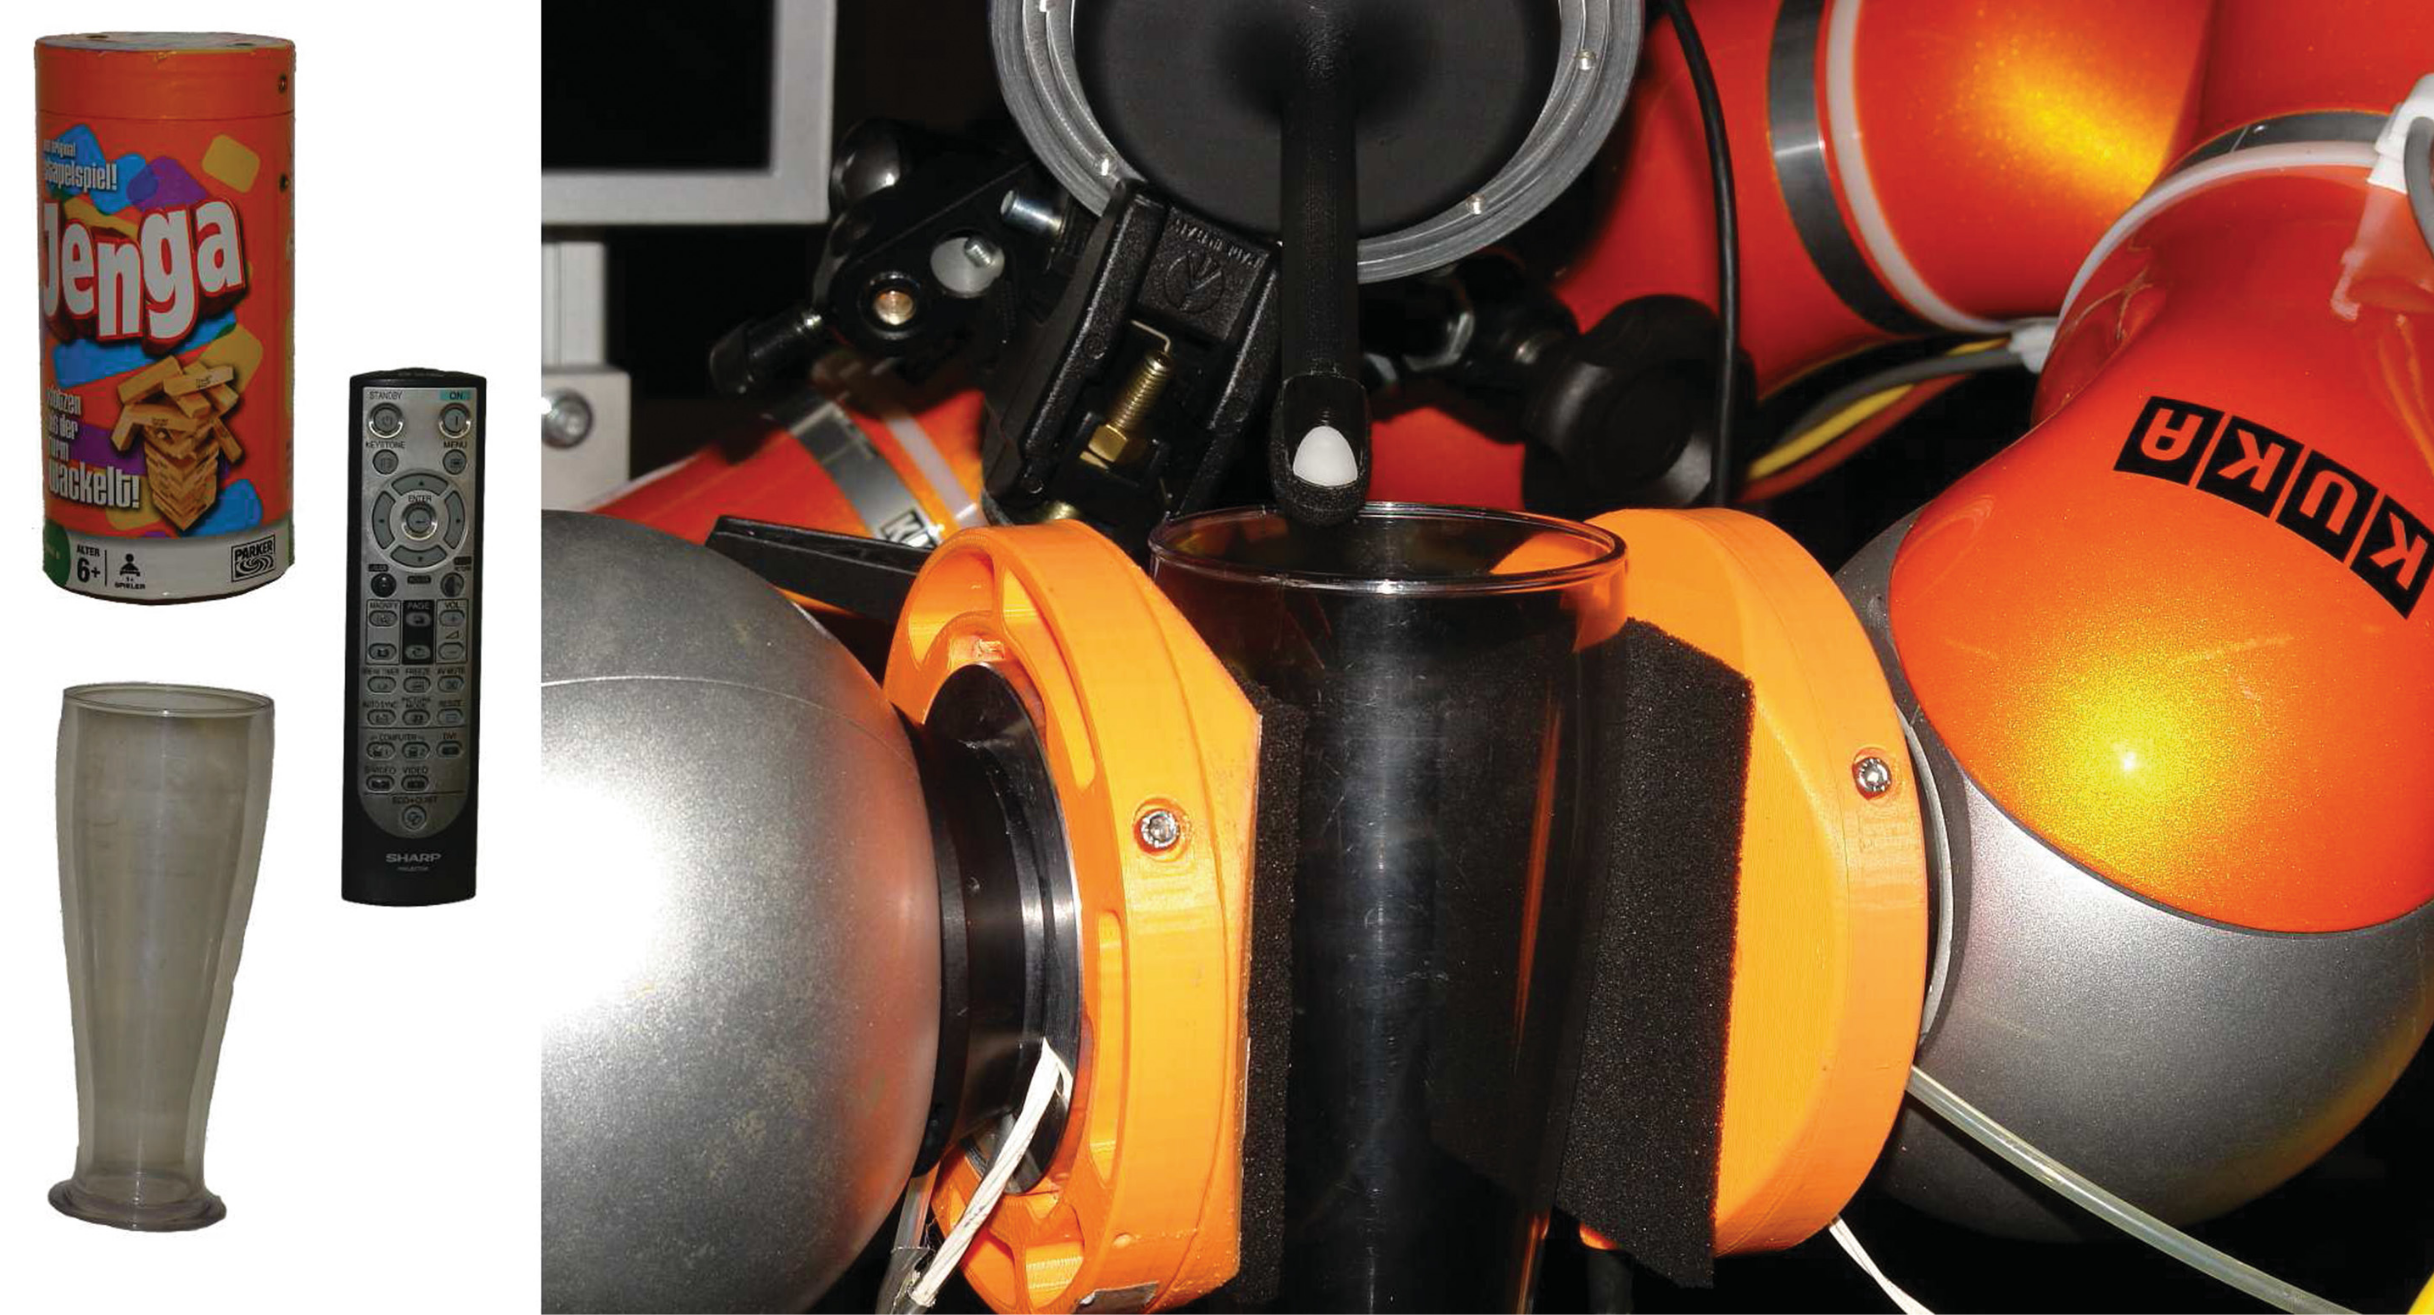
\includegraphics[width=\linewidth]{Figures/Tactile/meier2016.png}
    \caption{Objects and robotic setup of Meier \emph{et al.} approach \cite{Meier2016a}. Three different objects were used for training and evaluation: a can, a remote controller, and a glass. Two KUKA LWR robots with piezo-resistive sensor arrays are used to hold a glass. Figure extracted from \cite{Meier2016a}.}
    \label{fig:tactile:meier2016}
\end{figure}

In contrast, Cockbum \emph{et al.} \cite{Cockbum2017} proposed to use autoencoders to calculate the relevant characteristics for the task. Afterwards, a dictionary of basis features was built using a sparse encoding algorithm. Finally, the authors trained a \ac{SVM} in order to predict grasp stability using the dictionary. Similarly, Kwiatkowski \emph{et al.} \cite{Kwiatkowski2017} built a composite image by placing the readings of two matrix-like sensors side by side. Then, they used this tactile image as input for a \ac{CNN} along with the proprioceptive data from the robot. As a result, the proposed method calculated by itself the features needed for predicting grasp stability. Both of them used the same sensor (shown in Figure \ref{fig:tactile:kwiatkowski2017}): a custom-built array of $4\times 7$ tactels which rely on capacitive sensing to acquire static and dynamic variations in pressure over time.

\begin{figure}[!htb]
    \centering
    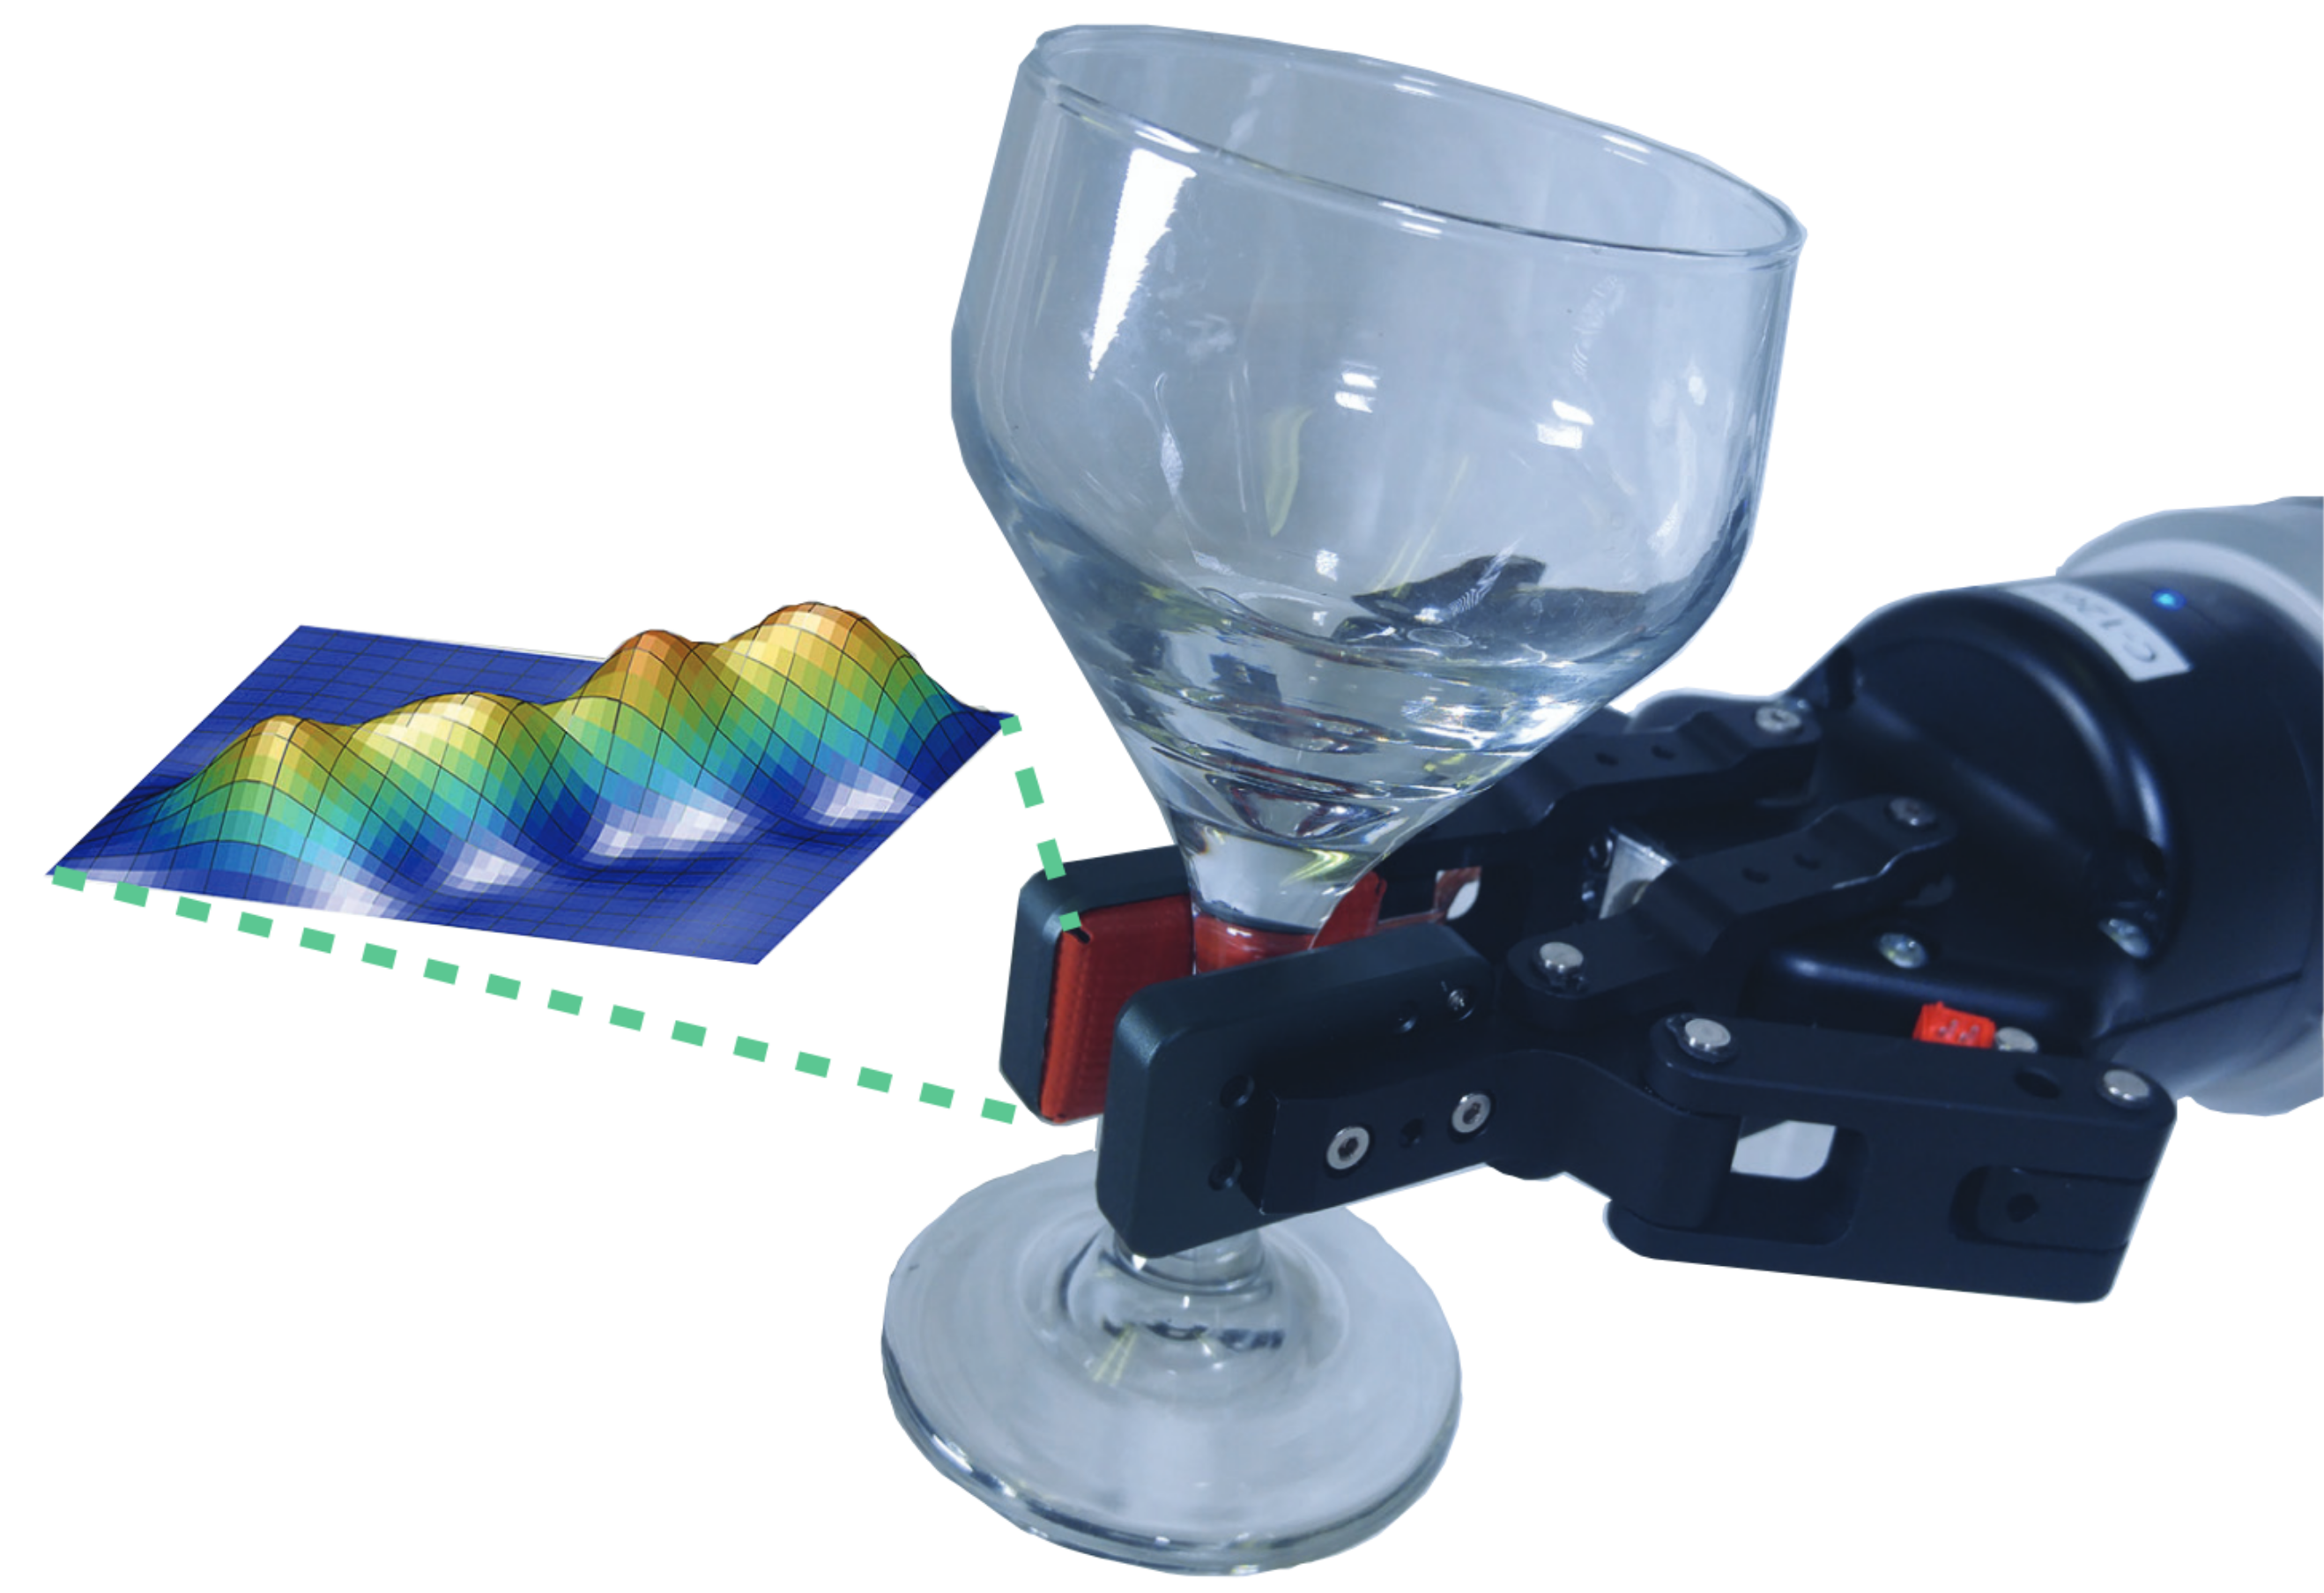
\includegraphics[width=0.8\linewidth]{Figures/Tactile/cockbum2017.png}
    \caption{Custom-built robotic gripper, used by Cockbum \emph{et al.}\cite{Cockbum2017} and Kwiatkowski \emph{et al.}\cite{Kwiatkowski2017}, with tactile sensors grasping a glass and the corresponding pressure image generated by one of them. Figure extracted from \cite{Kwiatkowski2017}.}
    \label{fig:tactile:kwiatkowski2017}
\end{figure}

There is an obvious trend in the field that suggests the interpretation of tactile sensors as images in order to exploit the potential of \ac{CNN} as spatial feature learners. In certain cases, even vision-based sensors are used for this purpose. Calandra \emph{et al.} \cite{Calandra2017} used a tactile sensor that contained an internal camera which recorded the deformation of the gel inside the sensor due to its contact with a surface. Some examples of tactile images collected by this sensor, namely GelSight, are shown in Figure \ref{fig:tactile:calandra2017}. The recorded tactile images were utilized to train a \ac{CNN} in order to predict the grasp outcome.

\begin{figure}[!htb]
    \centering
    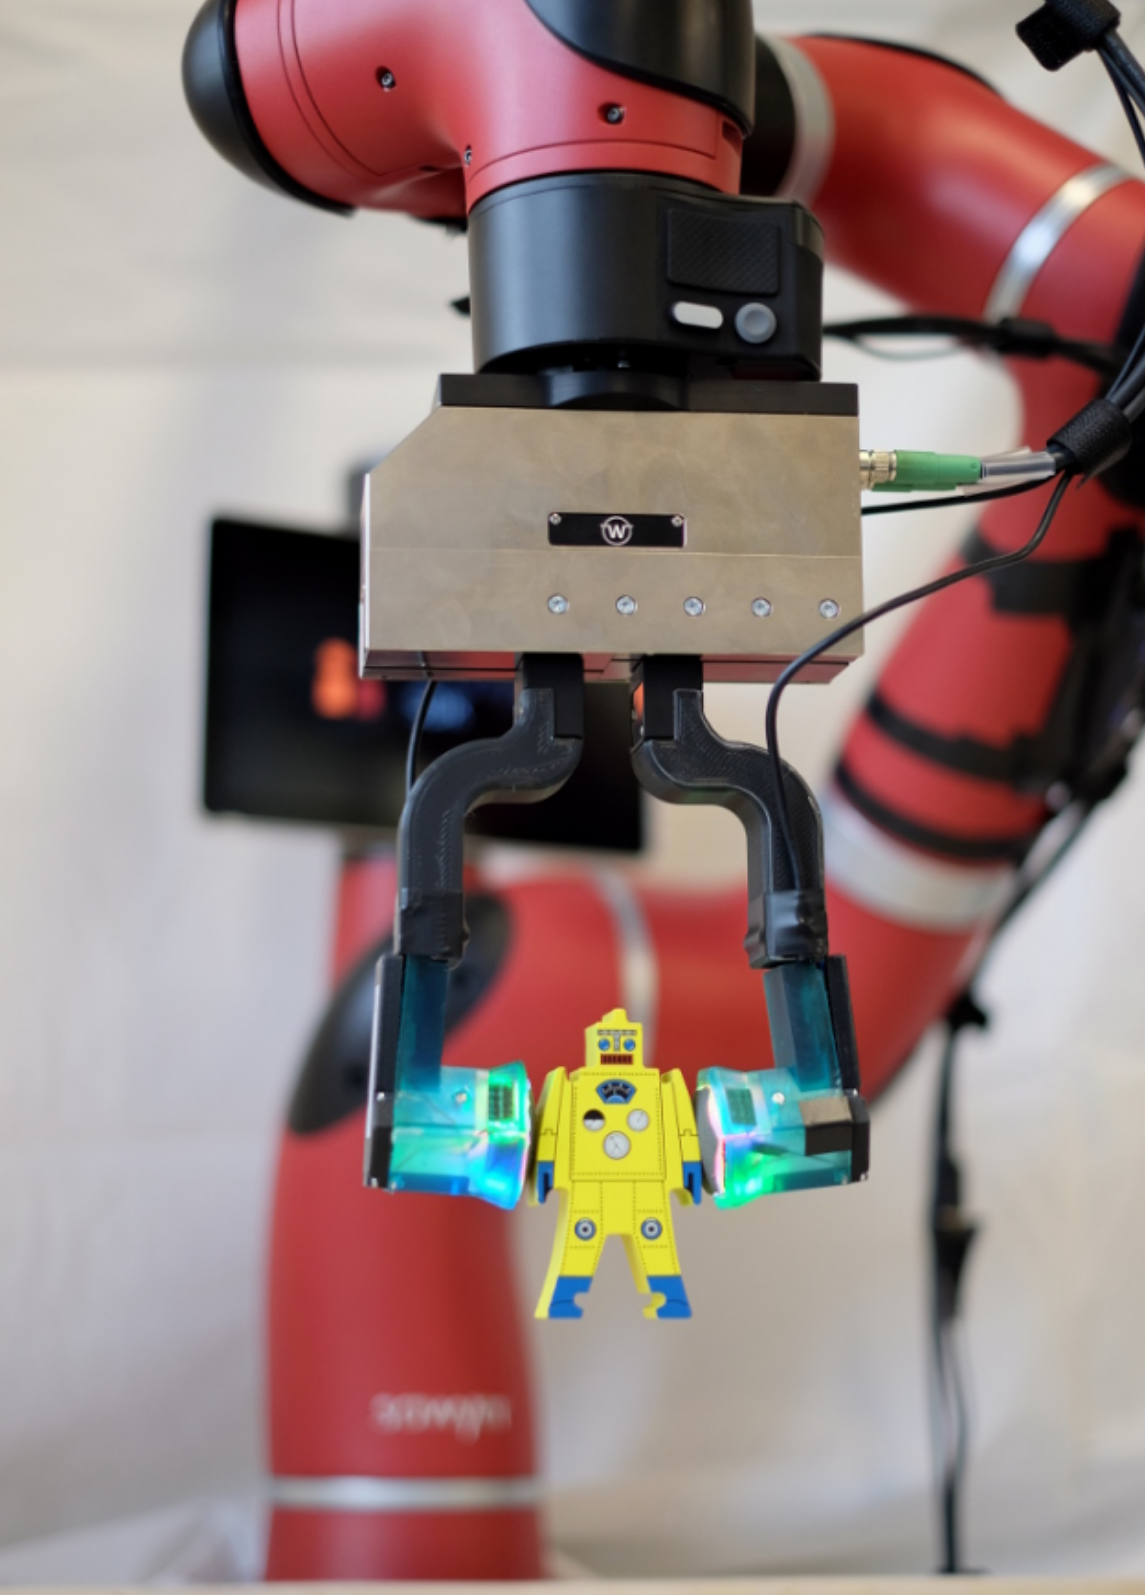
\includegraphics[width=0.21\linewidth]{Figures/Tactile/calandrarobot.png}
    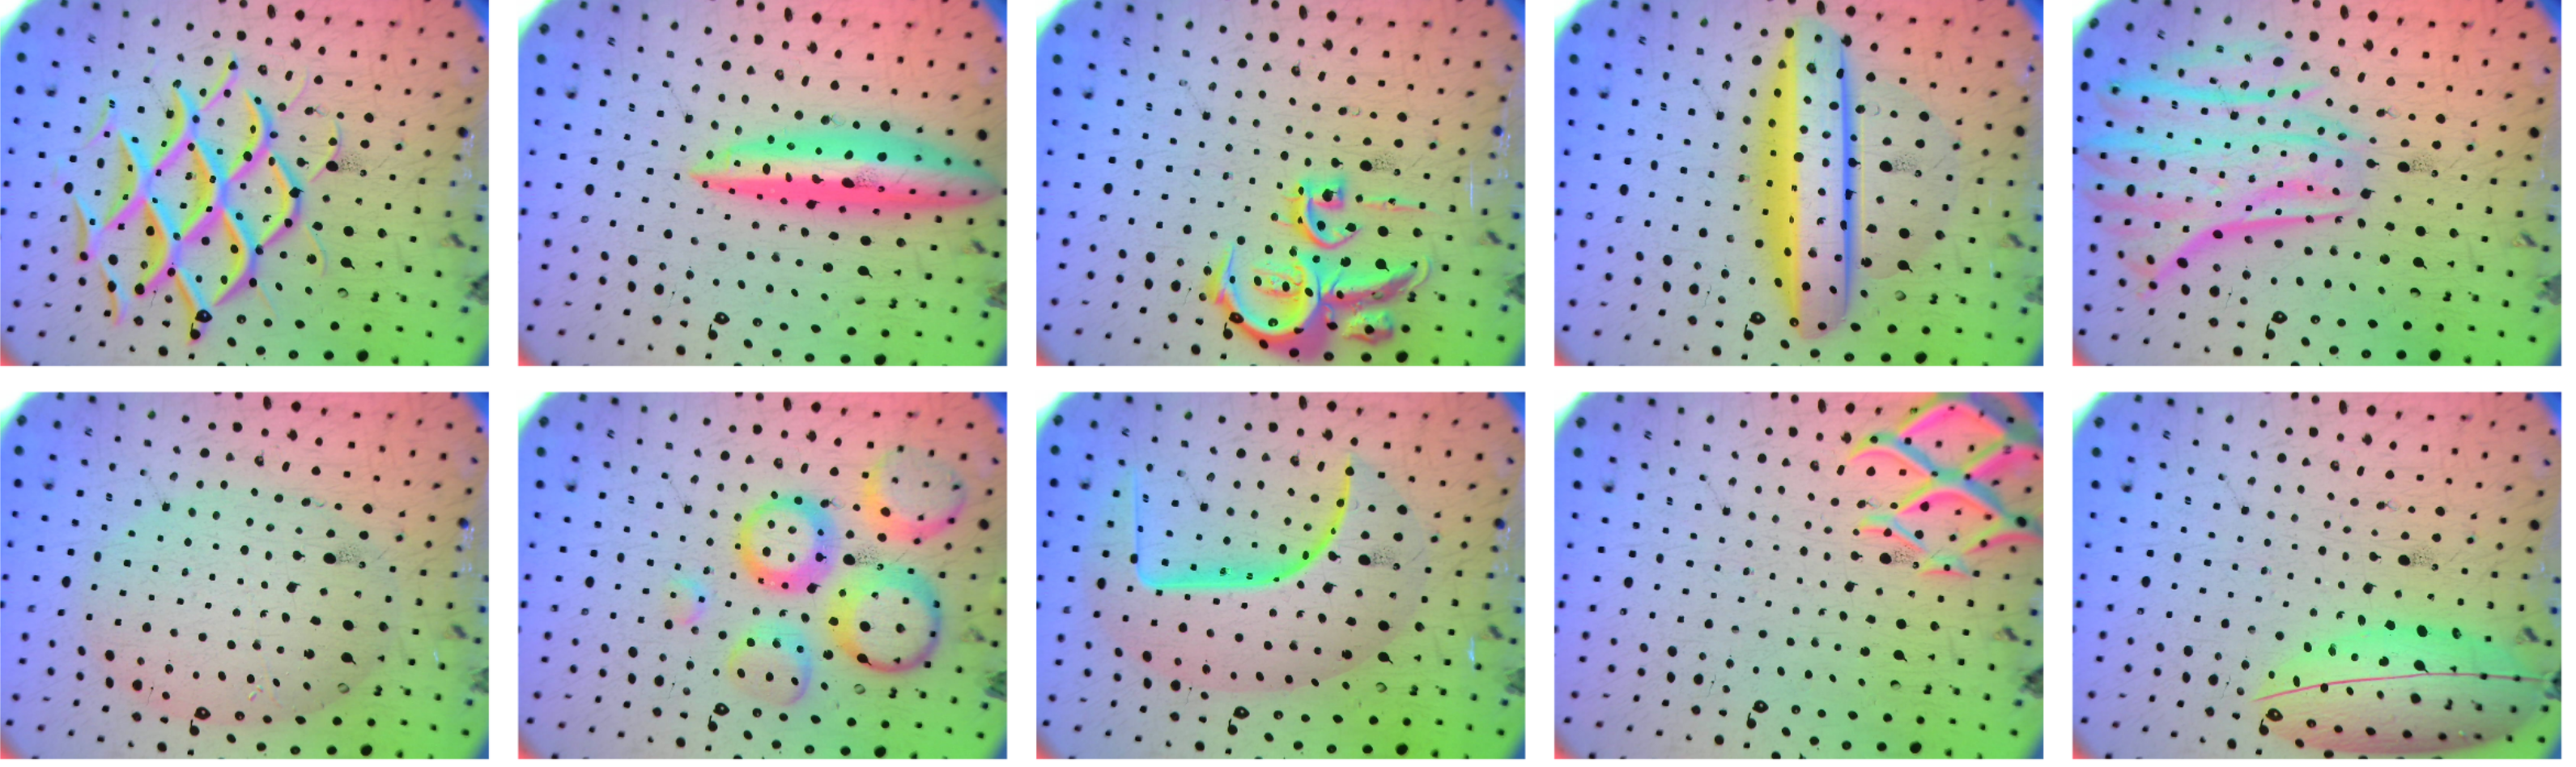
\includegraphics[width=0.78\linewidth, clip, trim=0 0 700 0]{Figures/Tactile/calandragelsight.png}
    \caption{Robotic gripper used by Calandra \emph{et al.}\cite{Calandra2017} and examples of raw tactile data capture by the custom-built GelSight camera embedded inside the tactile sensor. Figure extracted from \cite{Calandra2017}.}
    \label{fig:tactile:calandra2017}
\end{figure}

In some other cases, the tactile sensor is not naturally arranged in an array or it does not contain a camera. This is the case of the BioTacSP sensor \cite{Syntouch2018}. In this case, it is necessary to devise an arrangement and preprocess the tactile readings in order to generate a tactile image which can be fed to a \ac{CNN}. Zapata-Impata \emph{et al.} \cite{Zapata2018} studied how the readings from a non-matrix like sensor should be arranged in a matrix in order to train a \ac{CNN} for grasp stability prediction (see Figure \ref{fig:tactile:impata2018}). Although such approach showed promising results, the spatial distribution of the sensor was not accurately reflected because it reduced the \acs{3D} locations of the tactels into \acs{2D} coordinates of a tactile image.

\begin{figure}[!htb]
    \centering
    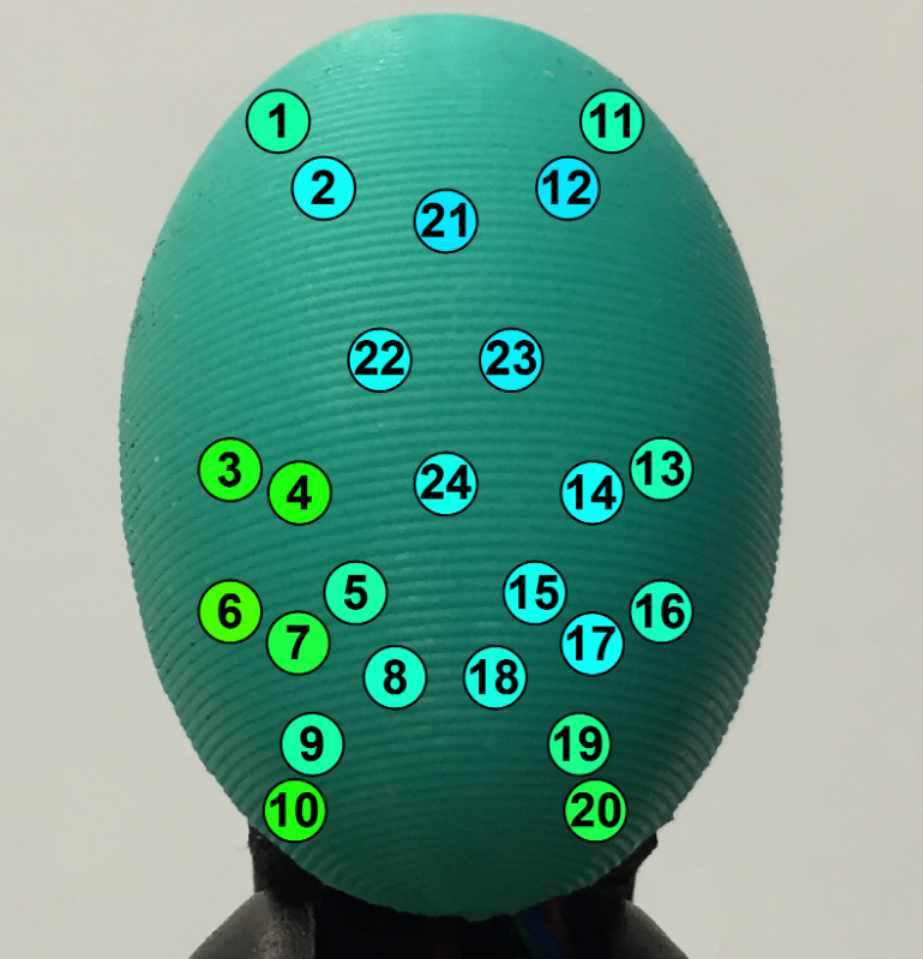
\includegraphics[width=0.3\linewidth]{Figures/Tactile/tactilebrayan1.png}
    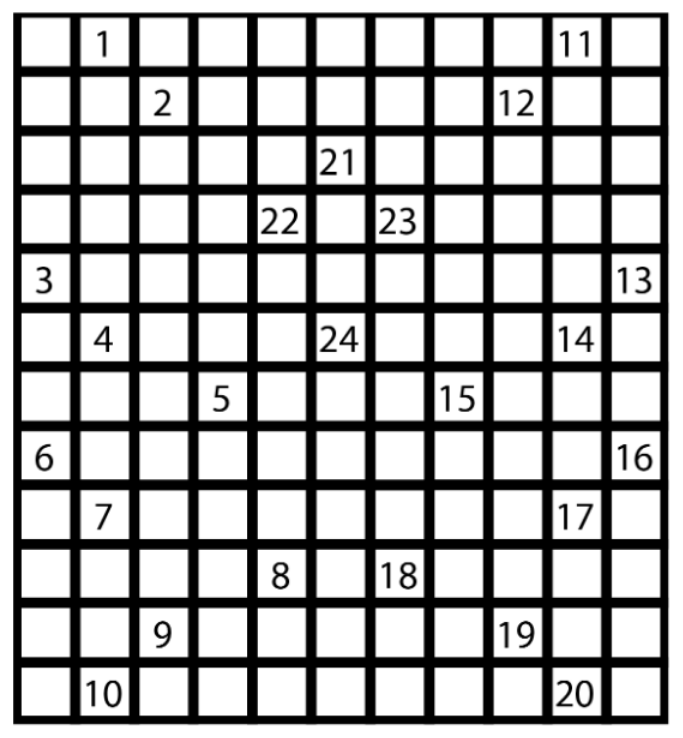
\includegraphics[width=0.3\linewidth]{Figures/Tactile/tactilebrayan2.png}
    \includegraphics[width=0.7\linewidth]{Figures/Tactile/tactilebrayan3.png}
    \caption{BioTacSp sensor used by Zapata-Impata \emph{et al.} and the corresponding tactile images generated from the sensor readings using a custom arrangement. Figure extracted from \cite{Zapata2018}.}
    \label{fig:tactile:impata2018}
\end{figure}

Recently, a novel trend aims to combine \acp{CNN} with \acp{LSTM} for grasp stability prediction to make them able to process spatio-temporal information. The hypothesis states that, although static information can be successfully used to predict stability, more useful information to better discriminate between stable and unstable grasps can be learnt from temporal data, e.g., whether the object is moving at a dangerous speed. Li \emph{et al.} \cite{Li2018} learnt visual features from a camera-based tactile sensor, similar to the one used by Calandra \emph{et al.} \cite{Calandra2017}, and an external camera pointing towards the scene. These features were calculated using a pre-trained \ac{CNN}. Then, both cameras features were concatenated and passed as time sequences to an \ac{LSTM}, which was in charge of predicting slippage. Similarly, Zhang \emph{et al.} \cite{Zhang2018} used another camera-based tactile sensor for grasp stability detection but in this work the authors trained a \ac{ConvLSTM} and they only passed the sensor images to the network.

\subsection{Grasp Stability Datasets}

Even though significant progress has been made in the area of grasp stability prediction, few publicly accessible datasets are available to enable the development (and fair comparisons) of realiable algorithms for predicting grasp stability using tactile information. Two of the most remarkable and recent works will be reviewed in this section: the \acf{BiGS}\footnote{\url{http://bigs.robotics.usc.edu/}} dataset \cite{Su2015b}, which makes use of the first BioTac sensors; and the BioTacSP Images\footnote{\url{https://github.com/yayaneath/biotac-sp-images}} dataset \cite{Zapata2018} that features the more recent BioTac SP sensor \cite{Syntouch2018}.

\begin{figure}[!htb]
    \centering
    \includegraphics[width=\linewidth]{Figures/Tactile/bigs}
    \caption{Sample grasp situations from the \ac{BiGS} dataset \cite{Su2015b}. A Barrett arm/hand system with three fingers equipped with BioTac sensors reaches to perform top grasps. It features box, cylindrical and spherical objects; the image shows two examples: cylindrical and box objects.}
    \label{fig:tactile:bigs}
\end{figure}

The \ac{BiGS} dataset \cite{Su2015b} features three objects: a cylindrically-shaped box of wipes, a cubically-shaped box of candy, and a spherically-shaped ball. It provides $1000$ grasps ($46\%/54\%$ failures/successes) for the cylindrical object, $500$ ($31\%/69\%$) for the box, and $500$ ($53\%/47\%$) for the spherical one. The dataset was recorded using a Barrett arm/hand system with three fingers in which each one of them is equipped with a BioTac sensor (an array of $19$ electrodes). To capture the data, the robot reaches for the object to perform a top grasp and then performs a range of extensive shaking motions. After that, if the object has fallen, it is considered to be a failed grasp; otherwise, it is considered to be a successful grasp. The dataset provides the following data: raw BioTac electrode values, BioTac pressure sensor values, robot's joint angles, end effector pose, BioTac temperature sensor values, and finger joint angles. Figure \ref{fig:tactile:bigs} shows some samples from this dataset.

\begin{figure}[!htb]
    \centering
    \includegraphics[width=\linewidth]{Figures/Tactile/biotacspimages}
    \caption{Sample grasps from the BioTacSP Images dataset \cite{Zapata2018}. Six different objects and two orientations (palm down and palm side) are shown. A Shadow hand is equipped with three BioTacSP sensors (thumb, middle, and index).}
    \label{fig:tactile:biotacspimages}
\end{figure}

The BioTacSP Images dataset \cite{Zapata2018} follows a similar approach but introduces more variety in shapes and objects. Furthermore, it makes use of the modern BioTacSP sensor (24 tactels) which is also equipped by three fingers in a humanoid Shadow hand (index, middle, and thumb). It contains $41$ objects and follows a similar methodology as \ac{BiGS} to determine if a grasp is successful or not. However, grasps were performed from two orientations: palm down (similar to the top grasp from \ac{BiGS}) and palm side. The dataset contains $1270$ stable grasps and $1279$ unstable ones and it is class-balanced with an average of $62$ grasps per class. For each grasps it provides the $24$ values from the sensor array: one for each tactel. Figure \ref{fig:tactile:biotacspimages} shows some grasping samples.

\subsection{Graph Neural Networks}
\label{cha:tactile:sec:relatedworks:subsec:gcns}

Lately, \acp{GNN} have emerged as a solid alternative to process irregular data which can be structured as graphs. Their original focus was tasks whose data can be expressed as graphs holding locality, stationarity, and composionality principles in general. In the literature, various works have successfully made use of this kind of architecture to deal with unstructured \acs{3D} representations mainly in classification tasks. Most of them  have proposed extensions to the well-known \ac{CNN} architecture to process graph-structured data. That generalization is not trivial since various problems must be addressed when applying convolution filters in domains in which there is no regular structure. In that regard, there are two dominant ways to convolve a graph signal with a learned filter: spatial or spectral.

Spectral methods are characterized by providing a spectral graph theoretical formulation of CNNs on graphs using Graph Signal Processing (GSP) theory \cite{Shuman2013}. The fundamentals of this kind of methods rely on decomposing the graph Laplacian to form a Fourier basis via an eigendecomposition of the graph matrix, i.e., a spectral decomposition. By doing that, a convolution in the graph domain can be expressed as a multiplication in the spectral one. This kind of methods usually faces three challenges: the design of compactly supported filters, the definition of parameter sharing schemes among different graphs, and the aggregation of multi-scale information. Arguably, the most common and limiting drawback is the first challenge: filters are not directly transferable to different graphs. Since filters are learned in the context of the spectrum of the graph Laplacian, a global graph structure must be assumed. In other words, only the signals on the vertices may change, the structure of the graph must remain the same.

Spatial methods constitute the straightforward generalization of convolutions to graph, just by sliding a filter on the vertices as a traditional CNN does with any other structured data representation. Despite its simplicity, the direct application of the definition of a convolution to graphs poses two difficulties: the definition of neighborhoods, and the ordering of the nodes to form receptive fields. Because of that, one common problem of spatial methods is the difficulty to generate a weight sharing schema across graph locations due to the fact that local neighborhoods can be completely different, i.e., the number of nodes adjacent to another one varies and there is no well-defined ordering for them.

Here we briefly review the most relevant \acp{GNN} that have been successfully applied to similar problems to the one at hand.

The pioneer spectral formulation of a CNN to operate over irregular domains modeled as graphs was introduced by Bruna et al. \cite{Bruna2013}. In that work, they exploited the global structure of the graph with the spectrum of its graph-Laplacian to extend the convolution operator. This method was applied to hand-written digit classification using the \ac{MNIST} dataset.

Defferrard \emph{et al.} \cite{Defferrard2016} proposed strictly localized filters, which are provable to be localized in a ball of a certain radius, i.e., hops from a specific vertex. That enhancement has some other collateral effects such as improved computational complexity for the filters (linear w.r.t. the support’s size and the number of edges). They also introduced an efficient  pooling strategy based on a rearrangement of the vertices as a binary tree. Their approach, namely \emph{Chebyshev Spectral Graph Convolutional Operator} or just \emph{ChebConv}, was successfully applied and performed similarly to classical \acp{CNN} in digits classification problems such as \acs{MNIST}.

Kipf and Welling \cite{Kipf2016} introduced a set of simplifications to Bruna's \cite{Bruna2013} and Defferrard's \cite{Defferrard2016} formulations to improve performance and scalability in large-scale networks. They proved the efficacy of their work on transductive node classification on very large scale networks for various problems such as semi-supervised document classification in citation networks (citeSeer, Cora and PubMed datasets) and semi-supervised entity classification in a knowledge graph (\acs{NELL} dataset). As its main feature, their \emph{GCNConv} operator takes advantage of fast localized first-order features to achieve linear scaling in the number of graph edges.

Simonovsky and Komodakis \cite{Simonovsky2017}, inspired by the idea from Jia \emph{et al.} [3] about dynamic filter networks, took a similar approach for solving the weight sharing problem suffered by spatial methods. They introduced \acp{ECC} in which filter weights are conditioned on edge features and generated by a generator network. That generator, usually implemented as a \ac{MLP}, outputs specific weights for each edge in the neighborhood. That method was successfully tested on point cloud classification problems (Sydney urban objects and ModelNet), a standard graph classification benchmarks, and also on \acs{MNIST}.

Velickovic \emph{et al.} \cite{Velickovic2017} introduced a \emph{Graph Attention} operator, namely \emph{GATConv}, that leverages masked self-attentional layers to compute the hidden representations of each node in the graph, by attending over its neighbors, following a self-attention strategy. This approach addressed many of the key challenges of spectral-based methods and achieved or surpassed state of the art methods in the aforementioned citation network datasets as well as protein interaction ones.

Fey \emph{et al.} \cite{Fey2018} proposed the \emph{Spline-based Convolutional Operator}, a continuous and spatial kernel that leverages B-spline bases's properties to efficiently filter graph data of arbitrary dimensionality. They prove this method to be successful in digit image graph classification problems using \acs{MNIST} and graph node classification using the Cora dataset.

Following this success in those similar domains, we intend to use a \acs{GNN} to process tactile sensor readings and predict grasp stability. By doing so, we expect that such architecture is able to better capture the spatial locality and relationships of the tactile sensor readings expressed as graphs instead of other non-spatial (\acs{1D} arrays) or discrete (images) representations.

\section{TactileGCN}
\label{cha:tactile:sec:tactilegcn}

In this section, we describe our full approach for predicting grasp stability using tactile sensors. The whole pipeline comprises three main components:

\begin{enumerate}
    \item A robotic setup which consists of a Shadow hand and BioTac Sp sensors, all operated by \ac{ROS}.
    \item A tactile graph generator which takes the sensor readings and generates a proper graph representation for the network.
    \item A \ac{GNN} architecture to process such graphs and predict graph stability.
\end{enumerate}

\subsection{Robotic Set Up}
\label{cha:tactile:sec:tactilegcn:subsec:rpobotic-set-up}

In this work, we use the BioTac SP tactile sensors developed by Syntouch \cite{Syntouch2018}. The sensor provides three different sensory modalities: force, pressure, and temperature. In more detail, this biomimetic sensor counts with $24$ electrodes, also named taxels, integrated in just a single phalanx. These electrodes record signals from four emitters in the internal core of the sensor and, therefore, they measure the impedance in the fluid located between the internal core and the external elastic skin of the sensor. The fluid is displaced when the sensor makes contact with a surface, affecting that impedance read by the electrodes. Thus, the sensor can approximate how much pressure is being experienced at each electrode. In addition, the sensor features a hydro-acoustic pressure sensor in order to estimate a general pressure value and it also counts with a thermistor, which is used to detect vibrations and heat flows. The sensor is presented in Figure \ref{fig:biotac-sensor}.

\begin{figure}[!htb]
	\centering
	\includegraphics[width = 0.26\textwidth, clip = true, trim = 0 75 0 20]{Figures/Tactile/biotac-sensor.png}
	\caption{BioTac SP tactile sensor with its 24 electrodes approximated position.}
	\label{fig:biotac-sensor}
\end{figure}

For our work, we use a setup of three BioTac SP sensors in the tip of the index, middle finger, and thumb of a Shadow Dexterous robotic hand developed by the Shadow Robot Company \cite{ShadowRobotCompany2018}. The Shadow hand is an anthropomorphic hand with five fingers and $20$ \ac{DoF} in total. Those features allow the robot to reach a wide range of configurations that are comparable to those of a human hand. Its integration with the BioTac SP sensors is seamless since the sensor readings can be directly obtained using the \ac{ROS} \cite{Quigley2009} framework, in which the Shadow hand works.

\subsection{Tactile Graphs}
\label{cha:tactile:sec:tactilegcn:subsec:tactile-graphs}

In order to feed our \acl{GNN}, we expressed the aforementioned sensor readings in a novel graph representation, namely tactile graphs. Such graphs are triplet $G = (N, E, Y)$ where $N$ is a set of $24$ nodes ${n_0, ..., n_{23}}$ (one for each electrode or taxel in the sensor), $E$ is a set of ordered pair of vertices called edges, and $Y$ is the label or class of the graph (in our case, stable or unstable).

Each node $n$ in the graph $G$ represents a taxel and as such, they are characterized by a \acs{3D} position $p_n = (x_n, y_n, z_n)$ and a feature vector $f_n = (f_{n_0}, ..., f_{n_F})$ of arbitrary length $F$.

Node positions $p_n$ are accurately mapped to the physical taxel $(X, Y, Z)$ coordinates within the sensor. Such positions are specified in Table \ref{table:taxel_coordinates}. Edges or connections are generated following two different approaches: manual or \ac{k-NN}. For the first approach, we manually specified undirected connections following proximity and symmetry criteria. For the second one, we generated directed edges towards each \acl{k-NN} for each node. Figure \ref{fig:graph_3d} shows a \acs{3D} graph representation of a tactile graph.

\begin{table}[!htb]
    \centering
    \caption{Actual position of the taxels inside the BioTac SP sensor expressed in Cartesian coordinates $(X,Y,Z)$ in inches.}
    \begin{tabular}{lccc}
        \hline
        \textbf{Taxel} & \textbf{X (inches)} & \textbf{Y (inches)} & \textbf{Z (inches)}       \\
        \hline
        1     & 0.386434851  & -0.108966104 & 0.156871012  \\
        2     & 0.318945051  & -0.205042252 & 0.120706090  \\
        3     & 0.087372680  & -0.128562247 & 0.281981384  \\
        4     & 0.083895199  & -0.235924865 & 0.201566857  \\
        5     & -0.018624877 & -0.300117050 & 0.094918748  \\
        6     & -0.091886816 & -0.120436080 & 0.284956139  \\
        7     & -0.136659500 & -0.237549685 & 0.187122746  \\
        8     & -0.223451775 & -0.270674659 & 0.071536904  \\
        9     & -0.320752549 & -0.199498368 & 0.127771244  \\
        10    & -0.396931929 & -0.100043884 & 0.151565706  \\
        11    & 0.386434851  & -0.108966104 & -0.156871012 \\
        12    & 0.318945051  & -0.205042252 & -0.120706090 \\
        13    & 0.087372680  & -0.128562247 & -0.281981384 \\
        14    & 0.083895199  & -0.235924865 & -0.201566857 \\
        15    & -0.018624877 & -0.300117050 & -0.094918748 \\
        16    & -0.091886816 & -0.120436080 & -0.284956139 \\
        17    & -0.136659500 & -0.237549685 & -0.187122746 \\
        18    & -0.223451775 & -0.270674659 & -0.071536904 \\
        19    & -0.320752549 & -0.199498368 & -0.127771244 \\
        20    & -0.396931929 & -0.100043884 & -0.151565706 \\
        21    & 0.258753050  & -0.252337663 & 0.000000000  \\
        22    & 0.170153841  & -0.274427927 & 0.072909607  \\
        23    & 0.170153841  & -0.274427927 & -0.072909607 \\
        24    & 0.075325086  & -0.298071391 & 0.000000000\\
        \hline
    \end{tabular}
    \label{table:taxel_coordinates}
\end{table}

\begin{figure}[!htb]
	\centering
    \includegraphics[width=0.8\linewidth]{Figures/Tactile/plot3d.png}
	\caption{3D visualization of the tactile graph layout using the accurate spatial arrangement from the actual BioTac SP sensor. Graph edges correspond to the manually defined connections.}
	\label{fig:graph_3d}
\end{figure}

Node features $f_n$ correspond to the taxel pressure readings. In the case of the most basic tactile graph, each node has three features, i.e., the pressure reading for each finger: index $f_{n_0}$, middle $f_{n_1}$, and thumb $f_{n_2}$. Figure \ref{fig:sample_graphs} shows visualizations of the three components of the feature vector for sample graphs generated with various values of $k=0$, $k=2$, $k=4$, $k=8$.

\begin{figure}[!htb]
    \centering
    \includegraphics[width=\linewidth, clip, trim={90 170 80 50}]{Figures/Tactile/plot-k0.png}
    \bigskip
    \includegraphics[width=\linewidth, clip, trim={90 190 80 50}]{Figures/Tactile/plot-k2.png}
    \bigskip
    \includegraphics[width=\linewidth, clip, trim={90 190 80 50}]{Figures/Tactile/plot-k4.png}
    \bigskip
    \includegraphics[width=\linewidth, clip, trim={90 10 80 50}]{Figures/Tactile/plot-k8.png}
	\caption{From top to bottom, undirected tactile graphs generated with various \ac{k-NN} configurations: $k=0$ (manually defined edges), $k=2$, $k=4$, and $k=8$. The three features (fingers) $f_{n_0}$, $f_{n_1}$, and $f_{n_2}$ are deocupled into three different plots and represented as contour plots in the XY plane. Nodes or taxels are shown as blue semi-transparent circles whose size depends on the pressure read on them. Undirected edges are represented by black lines. Features are color-coded in the range $[0, 4096]$.}
	\label{fig:sample_graphs}
\end{figure}

\subsection{\acl{GNN}}
\label{cha:tactile:sec:tactilegcn:subsec:gnn}

Our \acf{GNN} of choice is based on the \ac{GCN} model by Kipf and Welling \cite{Kipf2016}. Such model is arguably one of the most successful, yet simple, approaches to date to generalize a well-established model such as the \ac{CNN} to arbitrarily structured graphs \cite{Bronstein2017}\cite{Schlichtkrull2018}. Their proposal, which is somewhat similar to Defferard's \emph{et al.}, introduce a set of simplifications into a framework of spectral graph convolutions to make them train significantly faster and achieve state-of-the-art levels of accuracy across various classification tasks \cite{Defferrard2016}.

The goal of such models is to learn features on a graph $G = (N, E, Y)$ by taking as input a feature matrix $X$ ($N \times F$ with a feature vector $f_n$ for each node $n$) and a description of the graph structure in the shape of an adjacency matrix $A$ (computed from the set of edges $E$ in the graph). The output is another feature matrix $Z$ ($N \times F'$ with node-level feature vectors $f'_n$ with a predefined number of output features $F'$).

Each \ac{GCN} layer $H^(l)$ in a network with $L$ layers can be expressed as a non-linear function $H^{(l+1)} = f(H^{(l)}, A)$. The first layer takes the input feature matrix ($H^{(0)} = X$) and the final layer generates the output node-level feature matrix ($Z = H^{(L)}$). Each intermediate layer generates a node-level feature matrix $Z^{(l)}$ which is fed to the next layer. In the case of Kipf and Welling \cite{Kipf2016}, the graph-convolution layer $f(H^{(l), A)}$ is defined, in the most basic instantiation, as $\sigma(AH^{(l)}W^{(l)})$, where $\sigma$ is an activation function of choice and $W^{(l)}$ is the weight matrix for the $l$ layer.

This basic framework was heavily extended to overcome two limitations: (1) unless there are explicitly defined self-loops in the graph, the multiplication of $A$ only sums up the feature vectors of all the neighboring nodes but not the node itself, and (2) since $A$ is not normalized by default, the multiplication of $A$ has a huge impact on the scale of the feature vectors. Overcoming those two limitations is crucial to improve the model's convergence.

In order to fix those two limitations, they first enforced self-loops in the graph by adding the identity matrix to $A$ so the new adjacency matrix is $\hat{A} = A + I$. Secondly, they normalized that adjacency matrix in a row-like fashion by leveraging a symmetric normalization with the diagonal node degree matrix $\hat{D}$ of $\hat{A}$. Those two improvements combined form the layer propagation rule proposed by Kipf and Welling \cite{Kipf2016}: $f(H^{(l)}, A) = \sigma(\hat{D}^{-\frac{1}{2}}\hat{A}\hat{D}^{-\frac{1}{2}}H^{(l)}W^{(l)})$. This is the \emph{GCNConv} operator that we used to build our \ac{GNN}.

However, it is important to remark again that this model produces a feature matrix with node-level feature vectors yet our problem needs to classify the whole graph either as stable or slippery. To produce such binary graph-level classification output we need to introduce pooling operations to reduce the amount of nodes in the graph and/or fully connected layers to perform high-level reasoning.

\section{Experiments}
\label{cha:tactile:sec:experiments}

We conducted several experiments in order to validate our approach. In this section we describe the dataset we used to carry out such experiments. In addition, we provide all the details of our methodology to ensure the reproducibility of our procedures. At last, we discuss all the experiments that led us to the architecture described in the previous section.

\subsection{Dataset}
\label{cha:tactile:sec:experiments:subsec:dataset}

The dataset used in our experiments was first introduced in \cite{Zapata2018} as the \emph{BioTac SP Images} dataset. It contains grasp samples performed over $41$ objects with different geometries (i.e. cylinders, spheres, boxes), materials (i.e. wood, plastic, aluminum), stiffness levels (i.e. solid, soft) as well as sizes and weights. Those objects are shown in Figure \ref{fig:dataset_train}. For this work, added $10$ new objects with similar materials but different geometries and stiffness levels (see Figure \ref{fig:dataset_test}). The original $41$ were left for the training set whilst the new ones were separated into a test set. Both sets, training and test, were recorded following these steps:

\begin{enumerate}
	\item \textbf{Grasp the test object:} the hand performed a three-fingered grasp that contacted the object with each of the fingers equipped with a tactile sensor.	
	\item \textbf{Read the sensors:} a single reading was recorded then from each of the sensors at the same time.
	\item \textbf{Lift the object:} the hand was raised in order to lift the object and check the outcome.
	\item \textbf{Label the trial:} the previously recorded tactile readings were labeled according to the outcome of the lifting with two classes (stable, i.e., it is completely static, or slip, i.e., either fell from the hand or it moves within it).
\end{enumerate}

\begin{figure}[!htb]
	\centering
	\includegraphics[width=0.95\linewidth]{Figures/Tactile/dataset/trainobjects2-downsampled.jpg}
	\caption{The original training set of $41$ objects.}
	\label{fig:dataset_train}
\end{figure}

\begin{figure}[!htb]
	\centering
	\includegraphics[width=0.95\linewidth]{Figures/Tactile/dataset/testobjects.jpg}
	\caption{The newly captured test set of $10$ objects.}
	\label{fig:dataset_test}
\end{figure}

There are two hand configurations in the original dataset: \textit{palm down} grasps were performed pointing the palm of the hand downwards while \textit{palm side} grasps were recorded pointing it to one side, with the thumb upwards. In this work, we have added a new configuration: \emph{palm 45} which is in between the other two configurations at an angle of $45$ degrees. Figure \ref{fig:dataset_grasps} shows the aforementioned hand configurations.

\begin{figure}[!htb]
	\centering
    \includegraphics[width=0.32\linewidth]{Figures/Tactile/dataset/palmdown-downsampled}
    \includegraphics[width=0.32\linewidth]{Figures/Tactile/dataset/palmside-downsampled}
    \includegraphics[width=0.32\linewidth]{Figures/Tactile/dataset/palm45-downsampled}\\
    \smallskip
    \includegraphics[width=0.32\linewidth]{Figures/Tactile/dataset/palmdown_grasp-downsampled}
    \includegraphics[width=0.32\linewidth]{Figures/Tactile/dataset/palmside_grasp-downsampled}
    \includegraphics[width=0.32\linewidth]{Figures/Tactile/dataset/palm45_grasp-downsampled}
	\caption{(Top row) Samples of the three hand configurations in the dataset: (from left to right) \emph{palm down}, \emph{palm side}, and \emph{palm 45}. (Bottom row) The same configurations but grasping an object.}
	\label{fig:dataset_grasps}
\end{figure}

Table \ref{table:datasets} provides a quantitative summary of the extended dataset for both splits and all configurations.

\begin{table}[!htb]
	\renewcommand{\arraystretch}{1.3}
	\caption{Summary of the extended BioTac SP dataset which was used in this work to validate our graph-based architecture.}
	\label{table:datasets}
	\centering
	\begin{tabular}{lcccc}
        \hline
        & \multicolumn{2}{c}{\textbf{Training Set}} & \multicolumn{2}{c}{\textbf{Test Set}}\\
        \hline
        \textbf{Configuration} & \textbf{Stable} & \textbf{Slippery}  & \textbf{Stable} & \textbf{Slippery} \\
        \hline
        Palm Down & 667 & 609 & 153 & 163 \\
        Palm Side & 603 & 670 & 157 & 165 \\
        Palm 45 & 1058 & 1075 & 250 & 261 \\
        \hline
        All & 2328 & 2354 & 560 & 589 \\
        \hline           
	\end{tabular}
\end{table}

To the best of our knowledge, there is only one previous work that released a dataset of tactile recordings for the task of grasp stability detection, which is the BiGS dataset \cite{Chebotar2016bigs}. In their work, Chebotar \emph{et al.} recorded 2000 grasps on three standing objects (a cylindrically-shaped box of wipes, a cubically-shaped box of candy and a ball) using a Barret three-fingered hand, which was equipped with three BioTac tactile sensors. Our work extends the BioTac SP
dataset firstly introduced in \cite{Zapata2018}, counting with more than 4000 training grasps and 1000 test grasps with three BioTac SP tactile sensors recorded using 51 objects and various orientations, both for the objects and the hand. The dataset is freely available at GitHub \footnote{\url{https://github.com/3dperceptionlab/biotacsp-stability-set-v2}}.

\subsection{Experimental Setup}

All experiments were run on a computer with an i7-8700 CPU \@ $3.20$ GHz (6 cores / 12 threads) with an Z370 chipset motherboard, 16 GiB DDR4 RAM \@ $2400$ MHz CL15, a Samsung SSD 860 EVO 250 GiB, and an NVIDIA Titan X Maxwell (12 GiB) GPU. Everything was implement in Python $3.6$, PyTorch $0.4.1$, PyTorch Geometric $0.3.1$, CUDA $10.0$ (with driver version $410.73$).

For most experiments, we report accuracy as our main metric to iterate and draw conclusions over training and validation sets. For the test set, we report four different metrics: accuracy, precision, recall, and F1-score (the harmonic mean of precision and recall). To ensure generalization and give an accurate (and statistically correct) estimate of our prediction model performance we employ $k$-fold cross validation with $k=5$. All reported results are the average of $10$ rounds of $5$-fold cross validation. For each cross-validation split, we train our models for $512$ epochs using the ADAM optimizer. The hyperparameters were chosen empirically as follows: $0.01$ learning rate and $5e^{-4}$ weight decay.

The whole source code and dataset for this work can be downloaded from the corresponding GitHub repository\footnote{\url{https://github.com/3dperceptionlab/tactile-gcn}}.

\subsection{Network Depth and Width}

In these experiments, we investigate the impact of network depth (convolution layers) and width (amount of features per layer). To that end, we have tested ten different models ranging from one to ten \emph{GCNConv} layers with increasing number of features ($8$, $16$, $32$, $48$, $64$). ReLU activations were used after each convolutional layer. Two fully connected layers were also placed at the end of the network (with $128$ and $2$ output features respectively) to produce the classification
result. We made use of the manually defined graph connections ($k=0$). Figure \ref{fig:experiments_width_depth} shows the results of this set of experiments.

\begin{figure}[!htb]
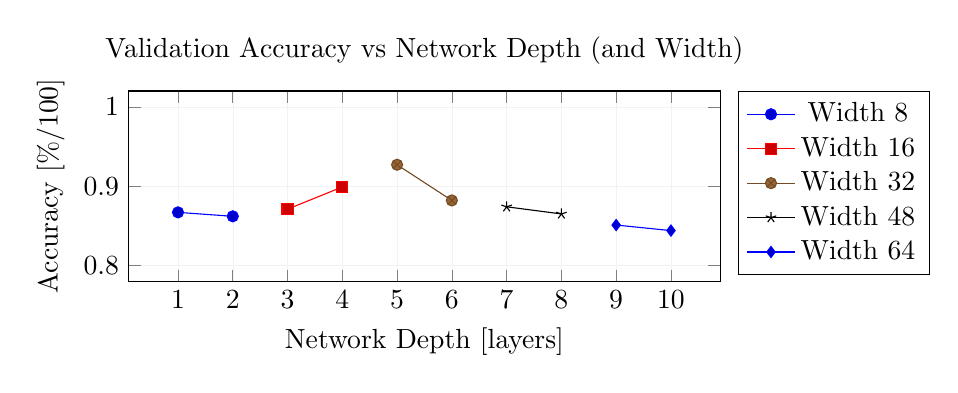
\begin{tikzpicture}
\begin{axis}[
    width=0.75\linewidth,
    height=4cm,
    title={Validation Accuracy vs Network Depth (and Width)},
    xlabel={Network Depth [layers]},
    ylabel={Accuracy [\%/100]},
    xmin=1, xmax=10,
    ymin=0.8, ymax=1,
    xtick={1, 2, 3, 4, 5, 6, 7, 8, 9, 10},
    ytick={0.0, 0.1, 0.2, 0.3, 0.4, 0.5, 0.6, 0.7, 0.8, 0.9, 1.0},
    legend pos=outer north east,
    grid style={line width=.1pt, draw=gray!10},
    ymajorgrids=true,
    xmajorgrids=true,
    enlargelimits=true,
]

  \addplot
    coordinates {
      (1, 0.867)(2, 0.862)
    };
  \addplot
    coordinates {
      (3, 0.871)(4, 0.899)
    };
  \addplot
    coordinates {
      (5, 0.927)(6, 0.882)
    };
  \addplot
    coordinates {
      (7, 0.874)(8, 0.865)
    };
  \addplot
    coordinates {
      (9, 0.851)(10, 0.844)
    };
  \legend{Width 8, Width 16, Width 32, Width 48, Width 64}
\end{axis}
\end{tikzpicture}
  \caption{Results of network depth and width study.}
  \label{fig:experiments_width_depth}
\end{figure}

As we can observe, there is a dependency on both width and depth. Shallow networks tend to perform better than their deep counterparts. However, we can find a sweet spot on the architecture with $5$ layers and $32$ features ($8-8-16-16-32$). Shallower networks are not able to fully capture our problem while deeper ones tend to overfit our training data. Consequently, we will proceed with that network.

\subsection{Graph Connectivity}

For the connectivity experiments we took the previous best network and investigated the effect of graph connectivity. We experimented with manually specified edges ($k=0$) and the \ac{k-NN} strategy with $k = [1, 23]$. As shown in Figure \ref{fig:experiments_connectivity}, the performance of the network degraded as the connectivity of the graph increased in each experiment. Using the \ac{k-NN} strategy, smaller $k$ values achieved greater performance in terms of validation accuracy. However,
none of them improved the performance ($92.7\%$) yielded by the network trained with the graph created using the manual connectivity ($k = 0$).

In the manually created graph there are electrodes connected by an edge to just one other electrode, some others are connected up to four neighbors and the electrode in the center (24th electrode) is connected to six other points. As a result, there are different degrees of connectivity within the graph that could have given some insight to the network about the importance of each node in order to better learn the problem.

\begin{figure}[!htb]
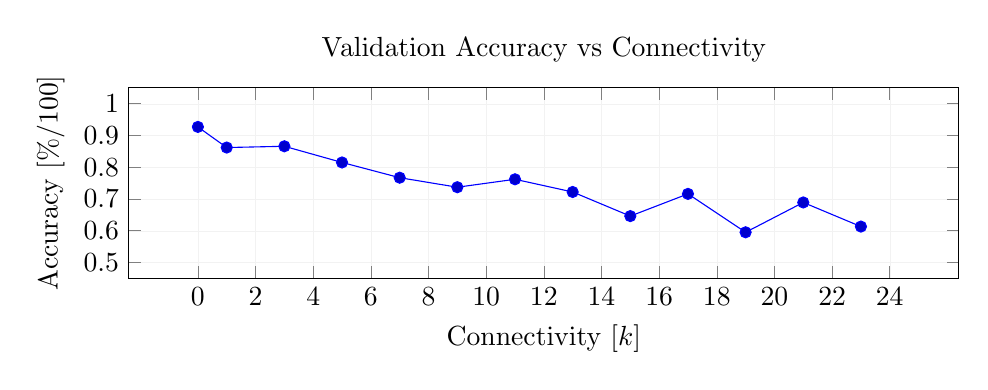
\begin{tikzpicture}
\begin{axis}[
    width=\linewidth,
    height=4cm,
    title={Validation Accuracy vs Connectivity},
    xlabel={Connectivity [$k$]},
    ylabel={Accuracy [\%/100]},
    xmin=0, xmax=24,
    ymin=0.50, ymax=1,
    xtick={0, 2, 4, 6, 8, 10, 12, 14, 16, 18, 20, 22, 24},
    ytick={0.0, 0.1, 0.2, 0.3, 0.4, 0.5, 0.6, 0.7, 0.8, 0.9, 1.0},
    grid style={line width=.1pt, draw=gray!10},
    ymajorgrids=true,
    xmajorgrids=true,
    enlargelimits=true,
]

  \addplot
    coordinates {
      (0, 0.927)(1, 0.862)(3, 0.866)(5, 0.815)(7, 0.767)(9, 0.737)(11, 0.762)(13, 0.722)(15, 0.646)(17, 0.716)(19, 0.595)(21, 0.689)(23, 0.613)
    };
\end{axis}
\end{tikzpicture}
  \caption{Performance of the network according to the connectivity of the graph.}
  \label{fig:experiments_connectivity}
\end{figure}

\subsection{Generalization Tests}

In order to prove the generalization capabilities of our system, we trained our best network ($8-8-16-16-32$ with $k=0$) with our whole training set and evaluated it on the various test sets (palm down, palm side and palm 45). All results are reported in Table \ref{table:generalization_tests}.

\begin{table}[!htb]
  \centering
    \caption{Results of generalization experiments on the testing splits.}
    \label{table:generalization_tests}
    \begin{tabular}{r|cccc}
        \hline
        \textbf{Test Set} & \textbf{Accuracy} & \textbf{Precision} & \textbf{Recall} & \textbf{F1}\\
        \hline
        Down & 0.741 & 0.741 & 0.751 & 0.745\\
        45 & 0.774 & 0.774 & 0.783 & 0.778\\
        Side & 0.751 & 0.785 & 0.709 & 0.745\\
        \hline
    \end{tabular}
\end{table}

There is a significant drop in accuracy when dealing with completely unknown objects. Recall that the test set consists of new objects with different geometries and stiffness levels so they are substantially different from the training set. Taking all of this into account, and despite the difficulty of the testing set, we can expect gains from applying regularization and augmentation strategies to increase performance on data whose distribution is not that similar to the training set.

\section{Conclusion}
\label{cha:tactile:sec:conclusion}

Tactile sensors provide useful information for robotic manipulation tasks like predicting grasp stability. Prior works in the literature tend to compute hand-engineered features that are later used for training a machine learning model. A recent trend process them as images, so deep learning techniques like \acsp{CNN} can calculate relevant characteristics that lets the system distinguish a slippery grasp from a stable one. Inspired by this methodology, we propose in this work a novel approach to tactile data interpretation: we build a graph with the sensor's taxels because this structure keeps more accurately the spatial distribution and the local connectivity of these sensing points. The goodness of these properties and the tactile graph for grasp stability prediction were tested in experimentation.

We used three BioTac SP tactile sensors mounted in the tip of the index, middle and thumb of a Shadow Dexterous hand. In order to predict grasp stability using these graph representations of the tactile sensors, we trained a \ac{GCN} with a custom dataset which was captured with more than 50 objects and 3 hand orientations. The robustness of the proposed system was checked by testing the system with novel orientations and objects. In average, the \ac{GCN} yielded a 92.7\% validation accuracy on the prediction of grasp stability with novel objects or orientations.

\subsection{Limitations and Future Works}
\label{cha:tactile:sec:conclusion:subsec:limitations}

Given the obtained results, graph representations of tactile readings can be successfully used for learning the task of grasp stability prediction. Nevertheless, there are some drawbacks linked to their used. The first limitation of this proposal is the problem of defining the graph connectivity. We had to find a way of defining the location of the taxels as well as their connections in order to define the graph. In the case of using the tactile readings directly, none of this is necessary.

Moreover, \ac{GCN} showed to be data hungry models for learning. In a previous work \cite{Zapata2018}, the authors obtained higher validation rates ($94.2\%$) with fewer data samples for training a \ac{CNN}. For this work, it was necessary to capture more data in order to achieve similar accuracy rates in training. Furthermore, generalization to radically new objects has still a lot of room for improvement by leveraging techniques such as L2 regularization, dropout, or data augmentation
itself.

As a future work, we also plan to decouple the currently unified \ac{GCN} for the three fingers so that each graph is processed by a different network path. Furthermore, we plan to model the noise of each individual taxel and augment each sample on the fly by adding random noise following each taxel's distribution. At last, we plan to extend the architecture to predict grasp stability over temporal sequences by fusing the \ac{GCN} model with \ac{LSTM} networks.
\chapter{Conclusion}
\label{cha:conclusion}

\begin{chapterabstract}
This last chapter of the thesis presents the final conclusions of this work. Firstly, Section \ref{cha:conclusion:sec:findings} presents the general conclusions of the work. Next, Section \ref{cha:conclusion:sec:contributions} goes through the major findings. At last, Section \ref{cha:conclusion:sec:future} concludes this thesis by listing the limitations of each one of the chapters in this thesis and also lists a set of possible future lines of research.
\end{chapterabstract}

\minitoc

\clearpage

\section{Conclusions}
\label{cha:conclusion:sec:findings}

In this thesis, we have explored four core problems for indoor robotics with a heavy emphasis on computer vision. However, despite the obvious differences and the distance between each topic, we can extract certain general conclusions.

First and foremost, after reviewing the state of the art of each of the topics of this thesis, we can state that deep learning has secured solid ground to be considered the \emph{de facto} paradigm for solving computer vision and robotics problems. In almost every aspect, deep learning architectures outperform traditional hand-engineered approaches.

A general observation across all problems is the fact that \ac{3D} representations offer useful information that is clearly beneficial for learning models with better generalization capabilities. However, to take full advantage of three-dimensional information, network architectures need to properly take into account the spatial arrangement and the unstructured nature of \ac{3D} data.

Following on the last observation, we also experienced the difficulties of training models for three-dimensional data. That additional dimension poses various challenges that range from memory footprint to increased execution time and also harder training prone to overfitting. In that regard, in order to ensure generalization, more quantity and more varied data is needed.

It is exactly at this spot where synthetic data generation is proven to be an extremely valuable tool to avoid the cost and errors of manually generated datasets. However, they still have to deal with problems of their own, mainly the transfer of the knowledge acquired in the synthetic domain to the real-world.

\section{Contributions}
\label{cha:conclusion:sec:contributions}

Once we have stated the general conclusions of the thesis, we briefly summarize the main contributions and findings.

Chapter \ref{cha:objrecog} introduced a set of networks and \acs{3D} data representations for the object classification problem. First, we proposed \emph{PointNet}: a \acl{CNN} architecture for \acs{3D} object classification which makes use of \acs{3D} representations such as point clouds or meshes by structuring them into an occupancy grid. Later, we tested an improved version under difficult conditions such as noise and occlusion to gain insight about real-world situations. At last, we presented our latest iteration, namely \emph{LonchaNet}, a novel slice-based model which significantly improves over other approaches. We show the performance of these models and prove their suitability for real time object classification.

In Chapter \ref{cha:semseg} we performed a comprehensive review of the state of the art of semantic segmentation for image and video using deep learning techniques. We provided an useful starting point for novel researchers and also enough details and depth so that more experienced ones could find it useful. Most importantly, apart from reviewing datasets and methods, we also gathered insights about weaknesses and future research.

One of the key observations that was made after the review was the scarcity of high-quality and large-scale datasets for data-driven algorithmms learning with \ac{3D} data. Following that train of thought, Chapter \ref{cha:sim2real} introduced a novel large-scale synthetic dataset for various robotic perception tasks with special focus on 3D semantic segmentation: \emph{the RobotriX}. Together with the data, we also released the full set of tools to generate it with detailed documentation.

Finally, Chapter \ref{cha:tactile} moved to the tactile sensing topic and showed a novel \acl{GNN} architecture which is able to classify the stability of robotic grasps using humanoid hands equipped with tactile sensors whose readings are interpreted as \acs{3D} graphs. We also demonstrated that this approach exhibits better generalization capabilities than previous methods based on more traditional architectures.

\section{Limitations and Future Work}
\label{cha:conclusion:sec:future}

To conclude this thesis, there are many aspects from the works presented here that can be improved in one way or another. Apart from those limitations to address, the work done here also raises questions that might spark important future work. Here we briefly highlight both limitations and future works.

\subsection{Object Classification}

\begin{itemize}
    \item Efficient and accurate representations for 3D data: although occupancy grids have been proven useful for the object classification task, they still present a set of disadvantages which renders them unsuitable for certain situations. One of the main weaknesses of such representation is the memory footprint which causes larger models that barely fit into \ac{GPU} memory for training if a considerable resolution is requested. Alternative sparse representations such as octrees or graphs might help but they would require new architectures to process them.
    \item Real-world datasets and deployment: our work has heavily focused on developing object recognition algorithms under certain conditions (fully isolated objects and synthetic models). Although we experimented introducing real-wolrd conditions such as noise and occlusions, it is still questionable whether or not the proposed models will behave properly in the real world. It would be interesting to check if such models can be trained or at least fine-tuned with smaller scale real-world object databases to measure their generalization capability.
\end{itemize}

\subsection{Semantic Segmentation}

\begin{itemize}
    \item Update datasets and methods: deep learning evolves at the speed of light and the hotness of the topic makes it difficult to maintain an up-to-date review. Since the writing of that chapter, various works have been published: novel datasets and environments and new methods, either iterations of the already presented ones or radically new concepts.
    \item Panorama and hyperspectral segmentation: despite the thoroughness of our review, some lines were intentionally left out due to the low relevance they presented at the moment. Some of those lines are panorama and hyperspectral images segmentation, which make use of a different input rather than common \ac{RGB} images.
    \item Real-time segmentation: with the growing complexity of deep learning models, they are becoming increasingly accurate but at the same time they are becoming heavier and slower. Most works focus on increasing the accuracy rate without taking into account that such models might need to be deployed into mobile solutions to be useful in a practical application. Recent works are following this line trying to streamline segmentation models that allow for real-time implementations while keeping good accuracy.
\end{itemize}

\subsection{Simulation to Real}

\begin{itemize}
    \item Non-rigid deformations: one limitation of our dataset and the tool itself that we use to generate it is that interactions are restricted to rigid objects. Non-rigid objects are not modeled so no deformations can occur. This is a challenging problem that might increase the usefulness of the dataset and the generation tool for many other robotic manipulation tasks.
    \item Random scene generation: one of the main flaws of our dataset is the limited amount of photorealistic scenes. This is due to the difficulty of designing a plausible scene and at the same time making sure that lighting, textures, and geometries look as realistic as possible. One possible way to improve or dataset would be to devise an algorithmic approach to generate this kind of scenes.
    \item Post-processing for increased realism: recently, many works have taken advantage of \acp{GAN} to augment datasets with subtle but realistic changes. We wonder if such kind of techniques could be used to improve the realism of the renders in an adversarial manner.
    \item Real-time raytracing: with the advent of the modern \acp{GPU} which feature hardware explicitly designed for carrying out raytracing operations it would be possible to raytracing in the generation phase to make scenes look even more realistic. Apart from the integration with the engine at hand, it also implies work on the art part (texturing and illumination setup).
\end{itemize}

\subsection{Tactile Sensing}

\begin{itemize}
    \item Graph topologies for the sensor readings: although it has been proven that generating a graph representation which better represents the actual topology of the tactels in a tactile sensor is useful, an open question remains: is it there a better topology? Further experimentation can be carried out to determine that. One possible line is learning the topology itself via a neural network, e.g., a \ac{GNG} \cite{Fritzke1999}.
    \item Temporal information for dynamic grasps: our proposal was focused on detecting if a given static grasp would be stable or not. However, objects are rarely such static entities but they are rather affected by many varying forces. In that regard, a promising future line of research would investigate the possibility of adding temporal information to a graph-based architectures. A possible way to do that would integrate other common recurrent architectures for such purpose such as \acl{LSTM}.
\end{itemize}

%----------------------------------------------------------------------------------------
%	THESIS CONTENT - APPENDICES
%----------------------------------------------------------------------------------------

\appendix % Cue to tell LaTeX that the following 'chapters' are Appendices

% Include the appendices of the thesis as separate files from the Appendices folder

%\input{Appendices/AppendixCaffeModels}
%\input{Appendices/AppendixSourceCode}

%----------------------------------------------------------------------------------------
%	BIBLIOGRAPHY
%----------------------------------------------------------------------------------------


\printbibliography[heading=bibintoc]

%----------------------------------------------------------------------------------------

\end{document}
